\documentclass[11p,a4paper,fleqn]{report}

\usepackage{amsmath}		                          %Matheschreibweise...
\usepackage{amssymb}                              %...Und Symbole
\usepackage{mathrsfs}                             %für Geogebra-Zeichnungen
\usepackage[T1]{fontenc}
\usepackage[margin=2cm]{geometry}	                %Seitenrand
\usepackage{fancyhdr}	                            %Header
%\usepackage{graphicx}	                          %Bilder einfügen
%\usepackage{wrapfig}                              %Text um Graphiken "wickeln" (wrap)
\usepackage[most]{tcolorbox}
\usepackage{tikz,pgf,pgfplots}                    %Grafiken zeichnen
\usepackage{mdframed}	                            %Box			%\begin{mdframed} 		und			%\end{mdframed}
\usepackage{epstopdf}
\usepackage[utf8]{inputenc}
\usepackage[ngerman]{babel}
\usepackage{tabu}                                 %Bessere Tabellen
\usepackage{esvect}                               %Schönere Vektoren
\usepackage{listings}                             %Für Pseudocode/Code...
\usepackage{color}                                %...Und dessen Einfärbung
\usepackage{enumitem}                             %Angepasstes enumerieren
\usepackage{enumerate}                            %Zeichen der Enumerierung beliebig wählbar
\usepackage[hidelinks=true]{hyperref}
\usepackage[makeroom]{cancel}                     %Durchgestrichene Terme mit \cancel{}
\usepackage{tkz-tab}                              %Für Monotonietabellen??
\usepackage{marvosym}                             %Symbole wie Blitze und co. ...
\usepackage{stackengine}                          %Zeichen übereinander "stapeln"
\usepackage{epigraph}                             %Fürs Titelblatt
%\usepackage{array}			                          %Gleichungen mit mehr als einem Zeichen in der Zeile oder Tabellen
\usepackage{tocloft,titletoc,titlesec}            %Fürs Inhaltsverzeichnis
\usepackage{flowfram}                              %Für die Seitenangabe
\usepackage{nopageno}                             %Same

\pgfplotsset{compat=1.14}
\usetikzlibrary{arrows}
%\usetikzlibrary{fit}

\nonstopmode                                      %Fehler bei Kompilierung werden "leise" gestellt (sehr viel praktischer)



\definecolor{titlepagecolor}{cmyk}{1,.60,0,.40}   %Blau

\def\blankpage{%
      \clearpage%
      \thispagestyle{empty}%
      \null%
      \clearpage}


\newlength{\lmargin}
\setlength{\lmargin}{1in + \hoffset + \oddsidemargin}
\newdynamicframe[odd]{2cm}{2cm}{-\lmargin}{6cm}[frameD-1a]
\newdynamicframe[even]{2cm}{2cm}{\textwidth+\lmargin-1cm}{6cm}[frameD-1b]

%%%%%%%%%%%%%%%%%%%%%%%%%%%%%%%%%%%%%%%%%%%%%%%%%%%%%%%%%%%%%%%%%%%%%%%%%%%%%%%%
%Für Kopf- und Fußzeilen:
\pagestyle{fancy}
\fancyhead[L]{\nouppercase{\leftmark}}
\fancyhead[R]{Skript SMP}
\fancyfoot[C]{\thepage}



%%%%%%%%%%%%%%%%%%%%%%%%%%%%%%%%%%%%%%%%%%%%%%%%%%%%%%%%%%%%%%%%%%%%%%%%%%%%%%%%%%%%%%
%Eigene Environments
%Beweis:
\newenvironment{Beweis}[1][]
  {\begin{tcolorbox}[colback=gray!5!white,colframe=gray!70!black,opacityframe=0.5, opacitybacktitle=0.5,sharpish corners,boxrule=0pt,frame hidden,title=Beweis \,#1,breakable,break at=23cm,pad at break=1mm,]}
  {\hfill\ensuremath{\square} \end{tcolorbox}}

%Definition:
\newenvironment{Definition}[1][]
  {\begin{tcolorbox}[colback=red!7!white,colframe=red!70!black,sharpish corners,boxrule=0pt,frame hidden,title=Definition \,#1]}
  {\end{tcolorbox}}

%Theorem:
\newenvironment{Theorem}[1][]
  {\begin{tcolorbox}[colback=titlepagecolor!5!white,colframe=titlepagecolor,sharpish corners,boxrule=0pt,frame hidden,title=Theorem \,#1]}
  {\end{tcolorbox}}

%Beispiel
\newenvironment{Beispiel}
  {\par\noindent\normalfont\par\nopagebreak%
  \begin{mdframed}[
     linewidth=2pt,
     linecolor=green,
     bottomline=false,topline=false,rightline=false,
     innerrightmargin=0pt,innertopmargin=0pt,innerbottommargin=0pt,
     innerleftmargin=1em,% Distanz zwischen vertikaler Strich & Inhalt
     skipabove=.5\baselineskip
   ]\underline{Beispiel:}\\}
{\end{mdframed}}

%Bemerkung
\newenvironment{Bemerkung}
  {\par\noindent\normalfont\par\nopagebreak%
  \begin{mdframed}[
     linewidth=2pt,
     linecolor=yellow,
     bottomline=false,topline=false,rightline=false,
     innerrightmargin=0pt,innertopmargin=0pt,innerbottommargin=0pt,
     innerleftmargin=1em,% Distanz zwischen vertikaler Strich & Inhalt
     skipabove=.5\baselineskip
   ]\underline{Bemerkung:}\\}
{\end{mdframed}}

%GTR-Tipp
\newenvironment{GTR-Tipp}
  {\par\noindent\normalfont\par\nopagebreak%
  \begin{mdframed}[
     linewidth=2pt,
     linecolor=gray,
     bottomline=false,topline=false,rightline=false,
     innerrightmargin=0pt,innertopmargin=0pt,innerbottommargin=0pt,
     innerleftmargin=1em,% Distanz zwischen vertikaler Strich & Inhalt
     skipabove=.5\baselineskip
   ]\underline{GTR-Tipp:}\\}
{\end{mdframed}}

%Codebox, aufrufbar mit \begin{lstlisting}[Name_der_Sprache]
\definecolor{dkgreen}{rgb}{0,0.6,0}
\definecolor{gray}{rgb}{0.5,0.5,0.5}
\definecolor{mauve}{rgb}{0.58,0,0.82}
\lstset{
  backgroundcolor = \color{lightgray},
  frame=tb,
  aboveskip=3mm,
  belowskip=3mm,
  showstringspaces=false,
  columns=flexible,
  basicstyle={\small\ttfamily},
  numbers=false,
  numberstyle=\tiny\color{gray},
  keywordstyle=\color{blue},
  commentstyle=\color{dkgreen},
  stringstyle=\color{mauve},
  breaklines=true,
  breakatwhitespace=true,
  tabsize=3
}

%Zahlenmengen-darstellung:
\newcommand{\N}{\mathbb{N}}
\newcommand{\Z}{\mathbb{Z}}
\newcommand{\R}{\mathbb{R}}
\newcommand{\C}{\mathbb{C}}
\newcommand{\Q}{\mathbb{Q}}
\newcommand{\P}{\mathbb{P}}
\newcommand{\A}{\mathbb{A}}
% "zu zeigen"-Zeichen mit \zz Quelle: http://www.matheboard.de/archive/155832/thread.html
\newcommand{\zz}{\mathrm{Z\kern-.3em\raise-0.5ex\hbox{Z}}}
% Achtung Zeichen mit \danger
\newcommand\danger[1]{
  \renewcommand\stacktype{L}
  \scaleto{\stackon[1.3pt]{\color{red}$\triangle$}{\tiny !}}{#1}
}
%Logarithmus dualis als "operator" angesehen mit \ld
\DeclareMathOperator{\ld}{ld}
%(Linke Seite)"Per definitionem äquivalent zu" (Ist halt die Frage, ob ich das richtig nutze)
\newcommand{\logEqL}{\ratio\Leftrightarrow}
%(Rechte Seite)"Per definitionem äquivalent zu"
\newcommand{\logEqR}{\Leftrightarrow\ratio}
%Linke Seite wird definiert zu / durch rechte Seite
\newcommand{\definedBy}{\ratio=}


%%%%%%%%%%%%%%%%%%%%%%%%%%%%%%%%%%%%%%%%%%%%%%%%%%%%%%%%%%%%%%%%%%%%%%%%%%%%%%%%%%%%%%
%Kapitel-Titelblatt
\makeatletter
\def\thickhrulefill{\leavevmode \leaders \hrule height 1.2ex \hfill \kern \z@}
\def\@makechapterhead#1{
  \vspace*{9\p@}%
  {\parindent \z@ \centering \reset@font
        \thickhrulefill\quad
        \huge\scshape\bfseries\textit{\@chapapp{}  \thechapter}\normalsize
        \quad \thickhrulefill
        \par\nobreak
        \vspace*{10\p@}%
        \interlinepenalty\@M
        \hrule
        \vspace*{10\p@}%
        \Huge \bfseries #1 \par\nobreak
        \par
        \vspace*{10\p@}%
        \hrule
  }
  %%HIER NAME DES AUTORS (KP WIE THO)
  \vskip 50\p@}

\setlength{\mathindent}{0pt}
\makeatother
\makeatletter
\newcommand{\chapterauthor}[1]{%
  {\parindent0pt\vspace*{-45pt}%
  \begin{flushright}
    \linespread{1.1} by \scshape#1%
  \end{flushright}
  \par\nobreak\vspace*{35pt}}
  \@afterheading%
}
\makeatother

%%%%%%%%%%%%%%%%%%%%%%%%%%%%%%%%%%%%%%%%%%%%%%%%%%%%%%%%%%%%%%%%%%%%%%%%%%%%%%%%
%Für den Titel:
\renewcommand\epigraphflush{flushright}
\renewcommand\epigraphsize{\normalsize}
\setlength\epigraphwidth{0.7\textwidth}
\DeclareFixedFont{\titlefont}{T1}{ppl}{b}{it}{0.5in}
\makeatletter
\def\printauthor{%
    {\large \@author}}
\makeatother
\author{%
    Clara Schaefer \\
    Bruno Gelfort \\
    Pascal Borel \\
    Rémy Moll \\
    [0,5cm]
    \textbf{1$^{ere}$ \& Te SMP}
    }
% The following code is borrowed from: https://tex.stackexchange.com/a/86310/10898
\newcommand\titlepagedecoration{%
\begin{tikzpicture}[remember picture,overlay,shorten >= -10pt]
\coordinate (aux1) at ([yshift=-15pt]current page.north east);
\coordinate (aux2) at ([yshift=-410pt]current page.north east);
\coordinate (aux3) at ([xshift=-4.5cm]current page.north east);
\coordinate (aux4) at ([yshift=-150pt]current page.north east);
\begin{scope}[titlepagecolor!40,line width=12pt,rounded corners=12pt]
\draw
  (aux1) -- coordinate (a)
  ++(225:5) --
  ++(-45:5.1) coordinate (b);
\draw[shorten <= -10pt]
  (aux3) --
  (a) --
  (aux1);
\draw[opacity=0.6,titlepagecolor,shorten <= -10pt]
  (b) --
  ++(225:2.2) --
  ++(-45:2.2);
\end{scope}
\draw[titlepagecolor,line width=8pt,rounded corners=8pt,shorten <= -10pt]
  (aux4) --
  ++(225:0.8) --
  ++(-45:0.8);
\begin{scope}[titlepagecolor!70,line width=6pt,rounded corners=8pt]
\draw[shorten <= -10pt]
  (aux2) --
  ++(225:3) coordinate[pos=0.45] (c) --
  ++(-45:3.1);
\draw
  (aux2) --
  (c) --
  ++(135:2.5) --
  ++(45:2.5) --
  ++(-45:2.5) coordinate[pos=0.3] (d);
\draw
  (d) -- +(45:1);
\end{scope}
\end{tikzpicture}%
}


%%%%%%%%%%%%%%%%%%%%%%%%%%%%%%%%%%%%%%%%%%%%%%%%%%%%%%%%%%%%%%%%%%%%%%%%%%%%%%%%
%Fürs Inhaltsverzeichnis:
%\contentsmargin{0cm}
\titlecontents{chapter}[0pc]
{\addvspace{40pt}
\begin{tikzpicture}[remember picture, overlay]%
\draw[fill=titlepagecolor,draw=titlepagecolor, rounded corners] (-4,-.1) rectangle (.5,.5);
\pgftext[left,x=-1.9cm,y=0.2cm]{\color{white}\Large \chaptertitlename\ \thecontentslabel};
\end{tikzpicture}\hspace{1cm}\color{titlepagecolor}\large\bfseries}
{}
{}
{\hspace*{20pt}\hrulefill\hspace*{20pt}\large\bfseries \thecontentspage}%\hspace*{20pt}\rule{1cm}{0.3pt}}%
[\addvspace{5pt}]








\makeatletter
\renewcommand{\tableofcontents}{
    \chapter*{}
    \@starttoc{toc}
    }
\makeatother


\usepackage[scale=.9]{helvet} % or tgheros
\renewcommand{\familydefault}{\sfdefault}
\setlength{\parindent}{0em}
\setlength{\parskip}{0em}

\begin{document}
  \begin{titlepage}

\begin{center}
	\hfill  \\
	[3,5cm]

	\titlefont Schülerskript SMP\\
	[0,5cm]
\end{center}
\epigraph{Mach' dir keine Sorgen wegen deiner Schwierigkeiten mit der Mathematik. Ich kann dir versichern, daß meine noch größer sind.}
{\textit{Brief an ein Schulmädchen, 1943}\\ \textsc{Albert Einstein}}
\null\vfill
\vspace*{1cm}
\noindent
\hfill
\begin{minipage}{0.35\linewidth}
    \begin{flushright}
        \printauthor
    \end{flushright}
\end{minipage}
%
\begin{minipage}{0.02\linewidth}
    \rule{1pt}{100pt}
\end{minipage}
\titlepagedecoration
\begin{center}
	\small{\today} \\
\end{center}
\end{titlepage}

  \blankpage
  \tableofcontents
  \begin{dynamiccontents*}{frameD-1a}
\begin{tikzpicture}
\draw(0,0) node [fill=titlepagecolor, minimum width=1cm, minimum height=1cm]{
{\sffamily\bfseries\large\color{white}\thepage}
};
\end{tikzpicture}
\end{dynamiccontents*}

\begin{dynamiccontents*}{frameD-1b}
\begin{tikzpicture}
\draw(0,0) node [fill=titlepagecolor, minimum width=1cm, minimum height=1cm]{
{\sffamily\bfseries\large\color{white}\thepage}
};
\end{tikzpicture}
\end{dynamiccontents*}

  %%%%%%%%%%%%%%%%%%%%%%%%%%%%%%%%%%%%%%%%%%%%%%%%%%%%%%%%%%%%%%%%%%%%%%%%%%%%%%
  %Kapitel bitte hier einbinden:
  \chapter{Folgen}
\chapterauthor{Clara}



\begin{Definition}
Eine Funktion, bei der nur natürlichen Zahlen eine reelle Zahl zugeordnet wird, nennt man Folge.\\
Folgen können auch nur für Teilbereiche von $\N$ definiert sein.\\
$(a_{n})_{n\in\N}$ bezeichnet die Folge, wobei $a:\N\rightarrow\R$
\end{Definition}

\begin{Bemerkung}
In einem Ausdruck muss das $n$ immer dasselbe bleiben!
\end{Bemerkung}


\begin{GTR-Tipp}
\\
Um statt Funktionen Folgen zu behandeln:
\begin{itemize}
\item\textcolor{gray}{ON} $\rightarrow \textcolor{red}{\text{MODE}} \rightarrow \text{Zeile 4: statt \textcolor{gray}{FUNC} \textcolor{red}{SEQ} auswählen}$
\item in \textcolor{gray}{Y=}
\item Mit $nMin$ den Startindex angeben
\item Mit $u(n)$ die Folgenvorschrift angeben
\item Falls die Folge rekursiv anzugeben ist, muss mit $u(nMin)$ das Startglied angegeben werden
\end{itemize}
\end{GTR-Tipp}

\begin{Bemerkung}
Es ist üblich eine rekursive Folge mit $a_{n+1}$ in Abhängigkeit von $a_n$ zu haben. Dies Darstellung ist mit dem GTR nicht direkt verwendbar. Man muss es "umschreiben" um $a_n$ in Abhängigkeit von $a_{n-1}$ zu haben.
\end{Bemerkung}

		\section{Verschiedene Darstellungen}


	\subsection{Explizite Darstellung}

\begin{Definition}
Wenn ein beliebiges Glied der Folge direkt berechenbar ist, ist ihre Darstellung explizit.
\end{Definition}

\begin{Beispiel}
\begin{enumerate}
\item  $a_{n}=3^n \Rightarrow a_{4}=3^4=81$
\item Die Folge der $n-ten$ positiven, ungeraden Zahl:\\
$a_{n}=1+2\cdot(n-1) \Rightarrow$ Die 8. positive, ungerade Zahl ist $ a_{8}=1+2\cdot(8-1)=15$
\end{enumerate}
\end{Beispiel}


	\subsection{Rekursive Darstellung}

\begin{Definition}
Wenn für die Berechnung des $n-ten$ Gliedes eines (oder sogar mehrere) der vorherigen Glieder benötigt wird, ist ihre Darstellung rekursiv.
In diesen Fällen braucht man immer ein Startglied, oft $a_{0}$ oder $ a_{1}$.
\end{Definition}

\begin{Beispiel}
\begin{enumerate}
\item  $a_{n}=3\cdot a_{n-1}+2;a_{0}=5$\\
\indent$a_{1}=3\cdot a_{1-1}+2=3\cdot a_{0}+2=3\cdot5+2=17$\\
\indent$a_{2}=3\cdot a_{2-1}+2=3\cdot a_{1}+2=3\cdot17+2=53$\\
\indent$a_{3}=3\cdot a_{3-1}+2=3\cdot a_{2}+2=3\cdot53+2=159$\\
\indent und so weiter...
\item Die Folge der $n-ten$ positiven, ungeraden Zahl:\\
$a_{n}=a_{n-1}+2;a_{1}=1$
\end{enumerate}
\end{Beispiel}

\begin{Bemerkung}
Für manche Folgen sind beide Darstellungen möglich, wobei die explizite Darstellung oftmals viel praktischer ist, da die Berechnung der Folgeglieder anhand der rekursiven Darstellung schnell sehr aufwendig wird.
\end{Bemerkung}

\subsubsection{Web-Diagramme}


Hier handelt es sich um ein graphisches Verfahren, das dazu dient, das Verhalten einer Folge, deren Darstellung rekursiv ist, zu untersuchen.  Es ermögicht die Beobachtung des Langzeitverhaltens (Konvergenz, Divergenz oder Oszillation) einer rekursiven Folge.\\\\
\begin{minipage}{0.5\textwidth}
Dazu muss man der rekursiven Folgenvorschrift eine \textcolor{blue}{Funktion $f(a_{n-1})=a_{n}$} zuordnen, sodass - grob gesagt - " die Funktion das Gleiche mit x macht, dass die Folge macht, um von $a_{n}$ auf $a_{n+1}$ zu kommen". Man muss verstehen, dass es sich hierbei nicht um den Graphen der Folge handelt, die Werte der Folgenglieder sind nicht wie gewohnt abzulesen. Zusätzlich zeichnet man in ein kartesisches Koordinatensystem die \textcolor{blue}{Hauptdiagonale} ein (entspricht dem Graphen von $f(x)=x$).  Exemplarisch wird hier die Folge $a_{n+1}=2\sqrt{a_n}+2$ behandelt, dementsprechend ist die Hilfsfunktion hier $f$ mit $f(x)=2\sqrt{x} +2$.
\end{minipage}
\begin{minipage}{0.5\textwidth}
	\definecolor{ttqqqq}{rgb}{0.2,0,0}
	\definecolor{sexdts}{rgb}{0.1803921568627451,0.49019607843137253,0.19607843137254902}
	\begin{tikzpicture}[line cap=round,line join=round,>=triangle 45,x=1cm,y=1cm,scale=0.5]
	\begin{axis}[
	x=1cm,y=1cm,
	axis lines=middle,
	ymajorgrids=true,
	xmajorgrids=true,
	xmin=-5.088547334373463,
	xmax=10.65108937607874,
	ymin=-3.575119239735864,
	ymax=9.474639170629912,
	xtick={-4,-2,...,22},
	ytick={-4,-2,...,10},]
	\clip(-5.088547334373463,-4.075119239735864) rectangle (22.65108937607874,10.874639170629912);
	\draw[line width=2pt,color=sexdts,smooth,samples=100,domain=2.505408374793447e-7:22.65108937607874] plot(\x,{2*sqrt((\x))+2});
	\draw[line width=2pt,color=ttqqqq,smooth,samples=100,domain=-5.088547334373463:22.65108937607874] plot(\x,{(\x)});
	\begin{scriptsize}
	\draw[color=sexdts] (0.8405353212957103,2.9444911186724285) node {$f$};
	\draw[color=ttqqqq] (-1.446396560176685,-3.1751691937860826) node {$Hauptdiagonale$};
	\end{scriptsize}
	\end{axis}
	\end{tikzpicture}
\end{minipage}


\begin{minipage}{0.5\textwidth}
\definecolor{rvwvcq}{rgb}{0.08235294117647059,0.396078431372549,0.7529411764705882}
\definecolor{ffqqqq}{rgb}{1,0,0}
\definecolor{ttqqqq}{rgb}{0.2,0,0}
\definecolor{sexdts}{rgb}{0.1803921568627451,0.49019607843137253,0.19607843137254902}
\begin{tikzpicture}[line cap=round,line join=round,>=triangle 45,x=1cm,y=1cm,scale=0.5]
\begin{axis}[
x=1cm,y=1cm,
axis lines=middle,
ymajorgrids=true,
xmajorgrids=true,
xmin=-1.7059310726041948,
xmax=13.731302722239086,
ymin=-1.91447455212563,
ymax=10.670477401431077,
xtick={-1,0,...,21},
ytick={-2,-1,...,10},]
\clip(-1.8059310726041948,-2.01447455212563) rectangle (21.731302722239086,10.670477401431077);
\draw[line width=2pt,color=sexdts,smooth,samples=100,domain=1.4376221380591118e-7:21.731302722239086] plot(\x,{2*sqrt((\x))+2});
\draw[line width=2pt,color=ttqqqq,smooth,samples=100,domain=-1.8059310726041948:21.731302722239086] plot(\x,{(\x)});
\draw [line width=2pt] (0,0)-- (0,2);
\draw [line width=2pt] (0,2)-- (2,2);
\draw [line width=2pt] (2,2)-- (2,0);
\begin{scriptsize}
\draw [fill=ffqqqq] (0,0) circle (2.5pt);
\draw[color=ffqqqq] (0.22437993412656146,0.3841672124633506) node {$a_0$};
\draw [fill=rvwvcq] (0,2) circle (2.5pt);
\draw[color=rvwvcq] (0.15251051795910106,2.378543511110368) node {$A$};
\draw [fill=rvwvcq] (2,2) circle (2.5pt);
\draw[color=rvwvcq] (2.146886816606127,2.378543511110368) node {$B$};
\draw [fill=ffqqqq] (2,0) circle (2.5pt);
\draw[color=ffqqqq] (2.2187562327735875,0.3841672124633506) node {$a_1$};
\end{scriptsize}
\end{axis}
\end{tikzpicture}
\end{minipage}
\begin{minipage}{0.5\textwidth}
Dann trägt man den Wert des ersten Folgegliedes auf die Abzissenachse ein und verbindet ihn mit der entsprechenden Funktion anhand eines vertikalen Striches. Der Ordinatenwert, der so erhalten wird (Punkt \textcolor{blue}{A}), entspricht dem Wert von $a_1$. Um den Vorgang erneuern zu können, muss der gefundene Wert wieder auf die Abzissenachse, dazu benutzt man die Hauptdiagonale als "Spiegel". Ein horizontaler Strich bis zur Hauptdiagonale (zum Punkt \textcolor{blue}{B})  und ein vertikaler bis zur Abzissenachse lösen das Problem. So ist der Wert von $a_1$ aud der Abzissenachse, dort wird er für den nächsten Schritt benötigt.
\end{minipage}
\\\\\\
Dasselbe muss mehrmals wiederholt werden, so wird jeweils das nächste Folgeglied auf die Abzissenachse abgebildet (\textcolor{red}{rote} Punkte). Daraus kann man dann eine \textcolor{blue}{Tendenz} erkennen\textcolor{blue}{, die die Entwicklung der Folgeglieder beschreibt}. Je nach dem, was für eine Tendenz zu erkennen ist, kann man verschiedene Schlüsse bezüglich der Entwicklung der Folge schließen. In diesem Falle wird deutlich, dass die Folge konvergiert, der Grenzwert ist die Schnittstelle zwischen der Hilfsfunktion und der Hauptdiagonalen, es fehlt nur noch diesen zu berechnen.
\\\\
%web2 weg
\begin{minipage}{0.6\textwidth}
\definecolor{ffqqqq}{rgb}{1,0,0}
\definecolor{ttqqqq}{rgb}{0.2,0,0}
\definecolor{sexdts}{rgb}{0.1803921568627451,0.49019607843137253,0.19607843137254902}
\begin{tikzpicture}[line cap=round,line join=round,>=triangle 45,x=1cm,y=1cm,scale=0.7]
\begin{axis}[
x=1cm,y=1cm,
axis lines=middle,
ymajorgrids=true,
xmajorgrids=true,
xmin=-1.6667190270420253,
xmax=12.536582509046294,
ymin=-1.3943671167960805,
ymax=8.554893100362574,
xtick={-1,0,...,17},
ytick={-1,0,...,8},]
\clip(-1.6667190270420253,-1.3943671167960805) rectangle (17.536582509046294,8.954893100362574);
\draw[line width=2pt,color=sexdts,smooth,samples=100,domain=3.636824072042055e-8:17.536582509046294] plot(\x,{2*sqrt((\x))+2});
\draw[line width=2pt,color=ttqqqq,smooth,samples=100,domain=-1.6667190270420253:17.536582509046294] plot(\x,{(\x)});
\draw [line width=2pt] (0,0)-- (0,2);
\draw [line width=2pt] (2,2)-- (2,0);
\draw [line width=2pt] (0,2)-- (2,2);
\draw [line width=2pt] (2,2)-- (2.0002386442865516,4.828595866705989);
\draw [line width=2pt] (2.0002386442865516,4.828595866705989)-- (4.832521331888258,4.832521331888258);
\draw [line width=2pt] (4.824827755036873,0)-- (4.834981558980159,6.397718298836414);
\draw [line width=2pt] (4.834981558980159,6.397718298836414)-- (6.4,6.4);
\draw [line width=2pt] (6.439718755130408,0)-- (6.400072931869821,7.059673085040108);
\draw [line width=2pt] (7.062828081198973,0)-- (7.050714692879745,7.310636381029959);
\draw [line width=2pt] (6.400072931869821,7.059673085040108)-- (7.048509591757752,7.054150668760428);
\draw [line width=2pt] (7.050714692879745,7.310636381029959)-- (7.312337285505,7.312337285505);
\draw [line width=2pt] (7.312337285505,7.312337285505)-- (7.337053956685568,0);
\begin{scriptsize}
\draw [fill=ffqqqq] (0,0) circle (2.5pt);
\draw[color=ffqqqq] (0.16565707372976055,0.35738443554168037) node {$a_0$};
\draw [fill=ffqqqq] (2,0) circle (2.5pt);
\draw[color=ffqqqq] (2.159282271369464,0.35738443554168037) node {$a_1$};
\draw [fill=ffqqqq] (4.824827755036873,0) circle (2.5pt);
\draw[color=ffqqqq] (4.988470970961102,0.35738443554168037) node {$a_2$};
\draw [fill=ffqqqq] (6.439718755130408,0) circle (2.5pt);
\draw[color=ffqqqq] (6.600961939640273,0.35738443554168037) node {$a_3$};
\draw [fill=ffqqqq] (7.062828081198973,0) circle (2.5pt);
\draw[color=ffqqqq] (7.231299318305767,0.35738443554168037) node {$a_5$};
\draw [fill=ffqqqq] (7.337053956685568,0) circle (2.5pt);
\draw[color=ffqqqq] (7.495161476816905,0.35738443554168037) node {$a_6$};
\end{scriptsize}
\end{axis}
\end{tikzpicture}
\end{minipage}
\begin{minipage}{0.4\textwidth}
$$h(x)=x; f(x)=2\sqrt{x}+2$$
$$h(x)=g(x)\Leftrightarrow x-2\sqrt{x}-2=0$$
$$\Rightarrow x_1=\left(\dfrac{2+\sqrt{12}}{2}\right)^2$$
$$g=x_1$$
\end{minipage}
\\\\\\
Es gibt andere mögliche Tendenzen, hier ein paar Beispiele:\\\\
\begin{minipage}{0.5\textwidth}
Die divergierende Treppe, es gibt also keinen Grenzwert, man kann den uneigendlichen Grenzwert aber ablesen, hier ist der Grenzwert der Folge $a_n$ mit $a_{n+1}=-\dfrac{3}{2}a_n-4$ und $a_0=5$: $-\infty$
\end{minipage}
\begin{minipage}{0.5\textwidth}
\definecolor{rvwvcq}{rgb}{0.08235294117647059,0.396078431372549,0.7529411764705882}
\definecolor{ffqqqq}{rgb}{1,0,0}
\definecolor{wrwrwr}{rgb}{0.3803921568627451,0.3803921568627451,0.3803921568627451}
\definecolor{ttqqqq}{rgb}{0.2,0,0}
\begin{tikzpicture}[line cap=round,line join=round,>=triangle 45,x=1cm,y=1cm,scale=0.5]
\begin{axis}[
x=1cm,y=1cm,
axis lines=middle,
ymajorgrids=true,
xmajorgrids=true,
xmin=-5.564895824577204,
xmax=10.351157204568363,
ymin=-8.78942481077331,
ymax=9.29739460798684,
xtick={-6,-4,...,28},
ytick={-8,-6,...,10},]
\clip(-7.064895824577204,-8.78942481077331) rectangle (28.351157204568363,10.29739460798684);
\draw[line width=2pt,color=ttqqqq,smooth,samples=100,domain=-7.064895824577204:28.351157204568363] plot(\x,{(\x)});
\draw[line width=2pt,color=wrwrwr,smooth,samples=100,domain=-7.064895824577204:28.351157204568363] plot(\x,{3/2*(\x)-4});
\draw [line width=2pt] (5,0)-- (4.999511757557879,3.4992676363368176);
\draw [line width=2pt] (4.999511757557879,3.4992676363368176)-- (3.490167444195548,3.490167444195548);
\draw [line width=2pt] (3.490167444195548,3.490167444195548)-- (3.493252072731324,0);
\draw [line width=2pt] (3.4921577126709917,1.2382365690064878)-- (1.2326800880447495,1.2326800880447495);
\draw [line width=2pt] (1.2326800880447495,1.2326800880447495)-- (1.2275059703280837,-2.1587410445078743);
\draw [line width=2pt] (1.2275059703280837,-2.1587410445078743)-- (-2.1638122523457697,-2.1638122523457697);
\draw [line width=2pt] (-2.1638122523457697,-2.1638122523457697)-- (-2.157820383689419,-7.2367305755341285);
\draw [line width=2pt] (-2.157820383689419,-7.2367305755341285)-- (-7.246229313030961,-7.246229313030961);
\draw [line width=2pt] (-2.157820383689419,-7.2367305755341285)-- (-2.172139496975313,0);
\begin{scriptsize}
\draw [fill=ffqqqq] (5,0) circle (2.5pt);
\draw[color=ffqqqq] (5.290170003147623,0.6593618561624863) node {$a_0$};
\draw [fill=ffqqqq] (3.493252072731324,0) circle (2.5pt);
\draw[color=ffqqqq] (3.803236479023191,0.6593618561624863) node {$a_1$};
\draw [fill=rvwvcq] (-7.246229313030961,-7.246229313030961) circle (2.5pt);
\draw[color=rvwvcq] (-6.875649739688639,-5.937215959952919) node {$J$};
\draw [fill=ffqqqq] (-2.172139496975313,0) circle (2.5pt);
\draw[color=ffqqqq] (-1.8741460676337316,0.6593618561624863) node {$a_3$};
\draw [fill=ffqqqq] (1.2307994510983928,0) circle (2.5pt);
\draw[color=ffqqqq] (1.5322834603604218,0.6593618561624863) node {$a_2$};
\end{scriptsize}
\end{axis}
\end{tikzpicture}
\end{minipage}



\begin{minipage}{0.5\textwidth}
\definecolor{ffqqqq}{rgb}{1,0,0}
\definecolor{wrwrwr}{rgb}{0.3803921568627451,0.3803921568627451,0.3803921568627451}
\definecolor{wvvxds}{rgb}{0.396078431372549,0.3411764705882353,0.8235294117647058}
\begin{tikzpicture}[line cap=round,line join=round,>=triangle 45,x=1cm,y=1cm,scale=0.8]
\begin{axis}[
x=1cm,y=1cm,
axis lines=middle,
ymajorgrids=true,
xmajorgrids=true,
xmin=-1.4635665987461786,
xmax=8.87634424568403,
ymin=-1.6012600965995993,
ymax=6.32408946253023,
xtick={-1,0,...,15},
ytick={-1,0,...,7},]
\clip(-1.4635665987461786,-1.6012600965995993) rectangle (15.097634424568403,7.32408946253023);
\draw[line width=2pt,color=wvvxds,smooth,samples=100,domain=-1.4635665987461786:15.097634424568403] plot(\x,{4/(\x)+1});
\draw[line width=2pt,color=wrwrwr,smooth,samples=100,domain=-1.4635665987461786:15.097634424568403] plot(\x,{(\x)});
\draw [line width=2pt] (1,0)-- (1,5);
\draw [line width=2pt] (1,5)-- (5,5);
\draw [line width=2pt] (5,5)-- (5,0);
\draw [line width=2pt] (5,1.8)-- (1.8115586238362207,1.8115586238362207);
\draw [line width=2pt] (1.819217423943969,0)-- (1.819217423943969,3.1987476303564684);
\draw [line width=2pt] (1.819217423943969,3.1987476303564684)-- (3.188287472262904,3.188287472262904);
\draw [line width=2pt] (3.188287472262904,3.188287472262904)-- (3.182039920366344,0);
\draw [line width=2pt] (3.1864592764550546,2.255311821982552)-- (2.2426555359698286,2.2426555359698286);
\draw [line width=2pt] (2.2364079840732676,0)-- (2.2364079840732676,2.788582418094674);
\draw [line width=2pt] (2.2364079840732676,2.788582418094674)-- (2.791956440140071,2.791956440140071);
\draw [line width=2pt] (2.791956440140071,2.791956440140071)-- (2.792662064245665,0);
\begin{scriptsize}
\draw[color=wvvxds] (0.8120182746863592,7.267199840694417) node {$f$};
\draw [fill=ffqqqq] (1,0) circle (2.5pt);
\draw[color=ffqqqq] (1.1407138675155035,0.3140238385394505) node {$a_1$};
\draw [fill=ffqqqq] (5,0) circle (2.5pt);
\draw[color=ffqqqq] (5.1356295342081815,0.3140238385394505) node {$a_2$};
\draw [fill=ffqqqq] (1.819217423943969,0) circle (2.5pt);
\draw[color=ffqqqq] (1.9624528495883644,0.3140238385394505) node {$a_3$};
\draw [fill=ffqqqq] (3.182039920366344,0) circle (2.5pt);
\draw[color=ffqqqq] (3.3151616354621507,0.3140238385394505) node {$a_4$};
\draw [fill=ffqqqq] (2.2364079840732676,0) circle (2.5pt);
\draw[color=ffqqqq] (2.379643409717663,0.3140238385394505) node {$a_5$};
\draw [fill=ffqqqq] (2.792662064245665,0) circle (2.5pt);
\draw[color=ffqqqq] (2.935897489890061,0.3140238385394505) node {$a_6$};
\end{scriptsize}
\end{axis}
\end{tikzpicture}
\end{minipage}
\begin{minipage}{0.5\textwidth}
Die konvergierende Spirale, es gibt also einen Grenzwert, den man erneut mit der Schnittstelle zwischen Funktion und Hauptdiagonale ermitteln kann. Hier konvergiert die Folge  $a_n$ mit $a_{n+1}=\dfrac{4}{a_n}+1$ und $a_1=1$
\end{minipage}

\begin{Bemerkung}
Dieses Verfahren kann ausschließlich bei rekusiven Folgen angewendet werden, bei denen keine zusätzliche Abhängigkeit von $n$ vorliegt (Beispiel: $a_{n}=3\cdot a_{n-1}+3+4\cdot n$) oder die Rekursivitätsebene den 1. Grad überschreitet, was bedeutet, dass $a_{n}$ nicht nur in Abhängigkeit von $a_{n-1}$ beschrieben wird, sondern von anderen Rekursivitätsebenen wie $a_{n-2}$ (Beispiel: die Fibonacci-Folge).\\
\end{Bemerkung}

\begin{GTR-Tipp}
\\
Mit den GTR ist dieses Verfahren auch möglich, die Arbeit der Fertigstellung der Striche wird vom Rechner übernommen. Das Bild ist vom Benutzer nur noch zu deuten, gegebenenfalls ist die Schnittstelle auszurechnen.
\begin{itemize}
\item Der Rechner muss auf \textcolor{red}{SEQ} stehen
\item in \textcolor{gray}{Y=} die rekursive Folge angeben
\item In \textcolor{gray}{2nd }\textcolor{red}{FORMAT} von \textcolor{gray}{Time} auf \textcolor{red}{Web} stellen
\item \textcolor{red}{TRACE} verwenden
\item Sooft auf \textcolor{gray}{ENTER} drücken, bis ausreichend Striche zu sehen sind.
\end{itemize}

\end{GTR-Tipp}


		\section{Auffällige Folgen}


	\subsection{Arithmetische Folgen}

\begin{Definition}
Eine Folge wird arithmetisch genannt, wenn die Differenz zweier aufeinander folgender Glieder konstant ist.
\begin{enumerate}
\item Rekursive Darstellung:\\
\indent $a_{n}=a_{n-1}+d$
\item Explizite Darstellung:\\
\indent Mit Startglied $a_{0}$: $a_{n}=a_{0}+n\cdot d$\\
\indent Mit Startglied $a_{1}$: $a_{n}=a_{1}+(n-1)\cdot d$\\
\indent Mit Startglied $a_{x}$: $a_{n}=a_{x}+(n-x)\cdot d$
\end{enumerate}
\end{Definition}

\begin{Bemerkung}
Letzteres gilt auch für beliebige Folgeglieder, also ist $a_{n}=a_{p}+(n-p)\cdot d;n,p\in\N$
\end{Bemerkung}

\begin{Beispiel}
$a_{n}=a_{n-1}+3;a_{0}=0\Leftrightarrow a_{n}=0+n\cdot3$
\end{Beispiel}

\begin{Bemerkung}
Jedes Folgeglied einer solchen Folge ist das arithmetische Mittel seines Vorgängers und Nachgängers: $a_{n}=\dfrac{a_{n-1}+a_{n+1}}{2}$
\end{Bemerkung}

	\subsection{Geometrische Folgen}

\begin{Definition}
Eine Folge wird geometrisch genannt, wenn der Quotient zweier aufeinander folgender Glieder konstant ist.
\begin{enumerate}
\item Rekursive Darstellung:\\
\indent $a_{n}=a_{n-1}\cdot q$
\item Explizite Darstellung:\\
\indent Mit Startglied $a_{0}$: $a_{n}=a_{0}\cdot q^n$\\
\indent Mit Startglied $a_{1}$: $a_{n}=a_{1}\cdot q^{n-1}$\\
\indent Mit Startglied $a_{x}$: $a_{n}=a_{x}\cdot q^{n-x}$\\
\end{enumerate}
\end{Definition}

\begin{Bemerkung}
Letzteres gilt auch für beliebige Folgeglieder, also ist $a_{n}=a_{p}\cdot q^{n-p};n,p\in\N$
\end{Bemerkung}

\begin{Beispiel}
$a_{n}=a_{n-1}\cdot3;a_{0}=2\Leftrightarrow a_{n}=2\cdot3^n$
\end{Beispiel}

\begin{Bemerkung}
Jedes Folgeglied einer solchen Folge ist das geometrische Mittel seines Vorgängers und Nachgängers:\\
 $a_{n}=\sqrt{a_{n-1}\cdot a_{n+1}}$
\end{Bemerkung}

		\section{Klassifizierung von Folgen}


	\subsection{Monotonie}

\begin{Definition}
Eine Folge $(a_n)_n\in\N$ heißt monoton \begin{cases} \text{\textcolor{red}{steigend/wachsend}}\\\text{\textcolor{orange}{fallend/abnehmend}}\end{cases} wenn \begin{cases} \textcolor{red}{a_n+1\geq a_n}\\\textcolor{orange}{a_n+1\leq a_n}\end{cases}.\\\\
Gelten dabei sagar \textbf{strikte} Ordnungsrelationen ($>$ oder $<$), dann ist $(a_n)$ \textbf{streng} monoton wachsend beziehungsweise abnehmend.

\end{Definition}

	\subsection{Beschränktheit}

\begin{Definition}
Man nennt eine  Folge $(a_n)n\in\N$ nach  \begin{cases} \text{\textcolor{red}{oben}}\\\text{\textcolor{orange}{unten}}\end{cases} \textbf{beschränkt}\\ wenn es eine Zahl  \begin{cases} \textcolor{red}{S\in\R}\\\textcolor{orange}{s\in\R}\end{cases} gibt mit  \begin{cases} \textcolor{red}{a_n\leq S}\\\textcolor{orange}{a_n\geq s}\end{cases} $\forall n\in\N$.\\\\
\textcolor{red}{$S$} ist eine \textcolor{red}{obere }Schranke\\
\textcolor{orange}{$s$} ist eine \textcolor{orange}{untere} Schranke
\end{Definition}

\begin{Definition}
Die kleinste obere Schranke ist das \textbf{Supremum} der Menge $\{a_n;n\in\N\}$.\\
Die größte untere Schranke ist das \textbf{Infimum} der Menge $\{a_n;n\in\N\}$.
\end{Definition}


\begin{Definition}
Eine nach \textbf{oben und unten} beschränkte Folge heißt \textbf{beschränkte} Folge (suite bornée).}
\end{Definition}

\begin{Beispiel}
\end{Beispiel}



	\subsection{Konvergenz}

\begin{Definition}
Eine Folge $(a_n)n\in\N$ ist konvergent, wenn sie einen Grenzwert besitzt.\\
Man sagt $a_n$ konvergiert gegen $g=\lim\limits_{n\to\infty}a_n$.
\end{Definition}



\begin{Theorem}

$$\lim\limits_{n\to\infty}a_n=g\Leftrightarrow \lim\limits_{n\to\infty}(a_n-g)=0$$
\end{Theorem}
\\
\underline{Wörtlich:} Eine Folge $(a_n)$ konvergiert gegen $g$ genau dann, wenn $(a_n-g)$ gegen den Wert $0$ konvergiert.
\subsubsection{Monotone Konvergenz}


\begin{Theorem}
Eine monotone Folge ist genau dann konvergent, wenn sie beschränkt ist.
\end{Theorem}

\begin{Beweis}
\end{Beweis}

Besser zu verstehen, wenn man zwei Fälle unterscheidet:

\begin{Theorem}
$$\exists\, S\in\R \quad \exists \,n_0\in\N \quad \forall n\geq n_0\,:\, a_n\leq a_{n+1}\; \land \; a_n\leq S$$
$$\Rightarrow \exists\, g\in\R \,:\, \lim\limits_{n\to\infty}a_n=g\;\land\; g\leq S $$
 \begin{center}und\end{center}
$$\exists \, s\in\R \quad\exists \, n_0\in\N \quad \forall n\geq n_0\,:\, a_n\geq a_{n+1}\; \land \;a_n\geq s$$
$$\Rightarrow \exists \, g\in\R \,:\, \lim\limits_{n\to\infty}a_n=g\;\land\; g\geq s$$
\end{Theorem}

	\underline{Wörtlicch:}
\begin{itemize}
\item Eine monoton \textbf{wachsende} Folge $(a_n)$ ist genau dann \textbf{konvergent}, wenn sie nach \textbf{oben beschränkt} ist. Ihr Grenzwert $g$ ist kleiner oder gleich der oberen Schranke $S\in\R$.
\item  Eine monoton \textbf{fallende} Folge $(a_n)$ ist genau dann \textbf{konvergent}, wenn sie nach \textbf{unten beschränkt} ist. Ihr Grenzwert $g$ ist größer oder gleich der oberen Schranke $s\in\R$.
\end{itemize}

\subsubsection{Divergenz}
\begin{Definition}
Eine Folge $(a_n)$, die keinen Grenzwert $g\in\R$ besitzt (nicht kovergiert), wird \textbf{divergent} genannt.\\\\
Kann man ihr trotzdem einen Grenzwert wie $\pm\infty$ zuordnen ist sie \textbf{bestimmt divergent}.\\
Besitzt die Folge überhaupt keinen Grenzwert, so heißt sie \textbf{unbestimmt divergent}.
\end{Definition}

\begin{Bemerkung}
Man nennt einen Grenzwert $g=+\infty$ oder $g=-\infty$ einen \textbf{uneigentlichen Grenzwert}.
\end{Bemerkung}


\subsubsection{Epsilon-n0-Definition}
\begin{Definition}
$$\lim\limits_{n\to\infty}a_n=g \ \Leftrightarrow\ \forall  \epsilon > 0\quad \exists\, n_0 \in\N \quad \forall n\geq n_0\,:\, |a_n-g|<\epsilon$$
\end{Definition}
\subsubsection{Grenzwertsätze}


Die Grenzwertsätze führen die Grenzwerte komplizierter Folgen auf einfachere Grenzwertbetrachtungen bekannter Folgen zurück.\\
\begin{Theorem}
\end{Theorem}

  \chapter{Reihen}
\chapterauthor{Clara}
\begin{Definition}
Eine Reihe ist eine Folge, deren Glieder die Partialsummen einer anderen Folge ist. Das bedeutet, dass das $n-te$ Glied der Reihe, die Summe der ersten $n$ Glieder einer anderen Folge ist. \\
Man hat also:

\begin{enumerate}
\item Mit Startglied $a_{0}$: $s_{n}=\sum\limits_{i=0}^{n-1}a_{i}$
\item Mit Startglied $a_{1}$: $s_{n}=\sum\limits_{i=1}^{n}a_{i}$
\item Mit Startglied $a_{x}$: $s_{n}=\sum\limits_{i=x}^{x+n-1}a_{i}$
\end{enumerate}

\end{Definition}

\begin{Bemerkung}
In manchen Fällen steht $s_{n}$ für die Partialsumme einer anderen Folge bis zum $n-ten$ Glied.
Dann gilt für ein beliebiges Startglied $a_{x}$ der Folge: $s_{n}=\sum\limits_{i=x}^{n}a_{i}$
\end{Bemerkung}

		\section{Artithmetische Reihen}

	\subsection{Gauß'sche Summenformel}

Die Gauß'sche Summenformel bezeichnet die Summe der $n$ ersten natürlichen Zahlen, also:\\
$1+2+3+...+n=\sum\limits_{k=1}^{n}k=\frac{n(n+1)}{2}$\\\\

\begin{minipage}[c]{0.5\textwidth}
	\underline{Begründung:}\\
	\begin{tabular}{c∣c∣c∣c∣c∣c∣c}
		&$1$&$2$&$3$&$4$&$...$&$n$\\\hline
		&$n$&$n-1$&$n-2$&$n-3$&$...$&$1$\\\hline
		$\sum$&$n+1$&$n+1$&$n+1$&$n+1$&$...$&$n+1$\\
	\end{tabular}
\end{minipage}
\begin{minipage}{0.5\textwidth}
So sieht man also, dass wenn man die vorher bestimmte Reihe mit sich selbst addiert (ein Mal davon "falschrum"), man $n$ Mal $n+1$ bekommt. Um dann den Wert einer einzelnen Reihe zu bekommen teilt man durch zwei.
\end{minipage}

\begin{Bemerkung}
Die Gauß'sche Summenformel ist ein Spezialfall der arithmetischen Reihe, ihre Glieder werden \textbf{Dreieckszahlen} genannt.
\end{Bemerkung}

\begin{Beweis}
Um zu beweisen, dass für alle $n\in\N$\\
$\sum\limits_{k=1}^{n}f(k)=g(n)$\\
 gilt, reicht es aus, \\
$g(n)-g(n-1)=f(n)$\\
 für alle positiven $n$ und\\
 $g(0)=0$\\
 zu zeigen. In der Tat trifft dies hier zu: \\
$g(n)-g(n-1)=\dfrac{n(n+1)}{2}-\dfrac{(n-1)n}{2}=\dfrac{n(n+1-n+1)}{2}=\dfrac{n\cdot 2}{2}=n=f(n)$ \\
für alle $n$ \\
und $g(0)=\dfrac{0\cdot 1}{2}=0$\\
\\
\underline{Quelle:} Wikipedia (Gaußsche Summenformel)\\
\end{Beweis}
\begin{Bemerkung}
Auch ein Beweis durch vollständige Induktion ist möglich, dieser wäre sogar empfehlenswert, da er einfacher durchzuführen ist: (Siehe Kapitel 8)
\end{Bemerkung}


	\subsection{Allgemein}

\begin{Definition}
Wenn $s_{n}$ die Summe der ersten $n$ Folgeglieder einer arithmetische Folge ist, heißt sie arithmetische Reihe.\\
Sei eine arithmetische Folge $a$ mit Startglied $a_{x}$ und $s$, die entsprechende Reihe, dann gilt\\
$s_{n}=\dfrac{n\cdot(a_{x}+a_{x+n-1})}{2}$
\end{Definition}

\begin{Bemerkung}
\begin{enumerate}
\item Am häufigsten wird verwendet:
\begin{itemize}
\item Mit Startglied $a_{0}$ : $s_{n}=\dfrac{n\cdot(a_{0}+a_{n-1})}{2}$
\item Mit Startglied $a_{1}$ : $s_{n}=\dfrac{n\cdot(a_{1}+a_{n})}{2}$
\end{itemize}
\item Alternativ kann auch folgende Darstellung verwendet werden:\\
$s_{n}=\dfrac{n\cdot(2a_{x}+(n-1)\cdot d)}{2}$
\end{enumerate}
\end{Bemerkung}

\begin{Beweis}
Sei eine arithmetische Folge $a$, mit Startglied $a_{x}$ und Differenz $d$, und $s$, die entsprechende Reihe, dann gilt\\
$s_{n}=a_{x}+a_{x+1}+a_{x+2}+...a_{x+n-1}\\
=a_{x}+(a_{x}+d)+(a_{x}+2d)+...+(a_{x}+(n-1)\cdot d})\\
=n\cdot a_{x}+d+2d+...+(n-1)\cdot d\\
=n\cdot a_{x}+(1+2+...+(n-1))\cdot d\qquad$	(Gauß)\\
$=n\cdot a_{x}+\dfrac{(n-1)\cdot n}{2}\cdot d\\
=n\cdot \dfrac{2a_{x}+(n-1)\cdot d}{2}\\
=n\cdot \dfrac{a_{x}+\overbrace{a_{x}+(n-1)\cdot d}^{a_{x+n-1}}}{2}\\
=n\cdot \dfrac{a_{x}+a_{x+n-1}}{2}$
\end{Beweis}

		\section{Geometrische Reihen}

\begin{Definition}
Wenn $s_{n}$ die Summe der ersten $n$ Folgeglieder einer geometrischen Folge ist, heißt sie geometrischen Reihe.\\
Sei eine geometrische Folge $a$ mit Startglied $a_{x}$ und $s$, die entsprechende Reihe, dann gilt\\
$s_{n}=\sum\limits_{i=x}^{n+x-1}a_{i}=a_{x}\cdot \dfrac{1-q^n}{1-q}$
\end{Definition}

\begin{Bemerkung}
\item Am häufigsten wird verwendet:
\begin{itemize}
\item Mit Startglied $a_{0}$ : $s_{n}=a_{0}\cdot \dfrac{1-q^n}{1-q}$
\item Mit Startglied $a_{1}$ : $s_{n}=a_{1}\cdot \dfrac{1-q^n}{1-q}$
\end{itemize}
\end{Bemerkung}

\begin{Beweis}
\underline{Allgemein:}\\
\\
$(1-q)(1+q+q^2+q^3+...+q^n)\\
=(1\textcolor{red}{-q)+(q}\textcolor{orange}{-q^2)+(q^2}\textcolor{green}{-q^3)+(q^3}\textcolor{brown}{-q^4)+.}.\textcolor{blue}{.+(q^n}-q^{n+1})\\
=1+(\textcolor{red}{-q+q})+(\textcolor{orange}{-q^2+q^2})+(\textcolor{green}{-q^3+q^3})+...+(\textcolor{blue}{-q^n+q^n})-q^{n+1}\\
=1-q^{n+1}$\\
\\
Man hat also $\sum\limits_{k=0}^nq^k=1+q+q^2+q^3+...+q^n=\dfrac{1-q^{n+1}}{1-q}$\\
Entsprechend ergibt sich $\sum\limits_{k=0}^{n-1}q^k=\underbrace{1+q+q^2+q^3+...+q^{n-1}}_{n\quad Summanden}=\dfrac{1-q^n}{1-q}$\\
\\
Somit gilt für eine Reihe $s$, die die Partialsumme einer geometrischen Folge $a$, mit Quotient $q$ und Anfangsglied $a_{x}$, ist, folgendes:\\
\\
$s_{n}=\sum\limits_{i=x}^{x+n-1}a_{i}\\
=a_{x}+a_{x+1}+a_{x+2}+...+a_{x+n-1}\\
=a_{x}+a_{x}\cdot q+a_{x}\cdot q^{2}+...+a_{x}\cdot q^{n-1}\\
=a_{x}\cdot(1+q+q^2+...+q^{n-1})\\
=a_{x}\cdot \sum\limits_{k=0}^{n-1}q^k\\
=a_{x}\cdot \dfrac{1-q^{n}}{1-q}$
\end{Beweis}

  \chapter{Funktionsuntersuchung}

Die \textbf{Analysis} (griechisch  análysis, deutsch "`Aufl"osung"') ist ein Teilgebiet der Mathematik.  Die Untersuchung von reellen und komplexen Funktionen hinsichtlich Stetigkeit, Differenzierbarkeit und Integrierbarkeit z"ahlt zu den Hauptgegenst"anden der Analysis. Die hierzu entwickelten Methoden sind in allen Natur- und Ingenieurwissenschaften von großer Bedeutung.\\

\section{Stetigkeit}

\begin{Definition}
Eine Funktion ist stetig an der Stelle $x_{0}$, wenn:
\begin{enumerate}
\item $x_{0}\in D$
\item $\lim\limits_{x \rightarrow x_{0}} {f(x)}$ existiert 
\item $\lim\limits_{x \rightarrow x_{0}^{\pm}} {f(x)}=f(x_{0})$\\
\end{enumerate}
\end{Definition}
Stetigkeit ist eine lokale Eigenschaft. Die Funktion $f$ hei�t dann stetig, wenn sie an jeder Stelle ihrer Definitionsmenge stetig ist.

\begin{Bemerkung}
Ist $f$ stetig und $I\subset \R$ ein reelles Intevall, dann ist $f(I)$ ebenfalls ein Intervall. Ist $f$ zudem streng monoton, so ist die Umkehrfunktion $f^{-1}$ ebenfalls stetig.
\end{Bemerkung}

\subsubsection{Stetige Fortsetzungen}

beim Vereinfachen von gebrochenrationalen Funktionen ist Vorsicht geboten, denn eine hebbare Definitionsl�cke ''aufzuheben" ver"andert den Definitionsbereich der Funktion. Die daraus resultierende Funktion wird \textbf{stetige Fortsetzung} genannt.

\section{Differenzierbarkeit}

Eine Funktion ist differenzierbar an der Stelle $x_{0} \in D$, wenn der beitseitige Grenzwert des Differenzenquotienten f"ur $h\rightarrow 0$ existiert. Anschaulich soll Die Funktion links und rechts des $x_{0}$ die selbe Ableitung haben. \\ 
\\
$\lim\limits_{h \rightarrow 0^{+}} {\dfrac{f(x_{0}+h)-f(x_{0})}{h}} = \lim\limits_{h \rightarrow 0^{-}} {\dfrac{f(x_{0}+h)-f(x_{0})}{h}} =f'(x_{0})$\\
\\
Dieser Grenzwert ist die \textbf{Ableitung} von $f$ an der Stelle $x_{0}$.\\
Die Funktion hei�t differenzierbar, wenn sie $\forall x \in D$ differenzierbar ist.\\
\\
Die Funktion $f(x)=|x|$ ist nicht differenzierbar, da bei der Stelle $x_{0}=0$ der linksseitige Grenzwert des differenzenquotienten ($\lim\limits_{h \rightarrow 0^{-}}{f'(x_{0})=-1$}) nicht mit dem rechtsseitigen Grenzwert (1) �bereinstimmt.\\

\subsection{Zusammenhang zwischen Stetigkeit und Differenzierbarkeit}

Ist eine Funktion $f$ an der Stelle $x_{0}$ differenzierbar, so ist sie an dieser Stelle auch stetig.
Die Umkehrung gilt erst einmal nicht, aber es gibt eine verneinende Aussage: Ist $f$ an der Stelle $x_{0}$ nicht stetig, so ist sie hier auch nicht differenzierbar.\\

\section{Ableitungsregeln}


Ein Ableitungswert gibt die Steigung an einem bestimmten Punkt an. Im Allgemeinen und zum Beweisen wird der Differentenquotient ben"otigt, um eine Ableitungsfunktion zu definieren, es geht aber in vielen F"allen schneller.

\subsection{Produktregel}

Sind die Funktionen $u$ und $v$ an der Stelle $x_{0}$ $\in$ $D$ differenzierbar, dann ist die Funktion $f(x)=u(x)\cdot v(x)$ bei $x_{0}$ auch differenzierbar und es gilt: \\
\\
$f'(x0) = u'(x_{0})v(x_{0})+u(x_{0})v'(x_{0})$\\

\begin{Beweis}
$
\begin{array}{rcl}
\lim\limits_{h \rightarrow 0} {\dfrac{f(x_{0}+h)-f(x_{0})}{h}} & = & \lim\limits_{h \rightarrow 0} {\dfrac{u(x_{0})v({x_{0}+h)-u(x_{0})v(x_{0})}}{h}}\\
&=&\lim\limits_{h \rightarrow 0} {\dfrac{u(x_{0}+h)v(x_{0}+h)\textcolor{red}{-u(x_{0})v(x_{0}+h)+u(x_{0})v(x_{0}+h)}-u(x_{0})v(x_{0}) }{h}}\\
&=&\lim\limits_{h \rightarrow 0} {\dfrac{u(x_{0}+h)v(x_{0}+h)-u(x_{0})v(x_{0}+h)}{h}} + \lim\limits_{h \rightarrow 0} {\dfrac{u(x_{0})v(x_{0}+h)-u(x_{0})v(x_{0})}{h}}\\
&=&\lim\limits_{h \rightarrow 0} {v(x_{0}+h)\dfrac{u(x_{0}+h)-u(x_{0})}{h}} \lim\limits_{h \rightarrow 0} {u(x_{0})\dfrac{v(x_{0}+h)-v(x_{0})}{h}}\\
&=& v(x_{0})\lim\limits_{h \rightarrow 0}{\dfrac{u(x_{0}+h)-u(x_{0})}{h}} +u(x_{0}) \lim\limits_{h \rightarrow 0} {\dfrac{v(x_{0}+h)-v(x_{0})}{h}}\\
&=& u'(x_{0})v(x_{0}) - u(x_{0})v'(x_{0}) 
\end{array}
$
\end{Beweis}

\subsection{Quotientenregel}

Sind die Funktionen $u$ und $v$ an der Stelle $x_{0}$ $\in$ $D$ differenzierbar, dann ist die Funktion $f(x)=\frac{u(x)} {v(x)}$ bei $x_{0}$ auch differenzierbar und es gilt: \\
\\
$f'(x_{0})=\frac{u'(x_{0})\cdot v(x_{0})-u(x_{0})\cdot v'(x_{0})}{v^2(x_{0})}$\\

\begin{Beweis}
$
\begin{array}{rcl}
\lim\limits_{h \rightarrow 0} {\dfrac{f(x_{0}+h)-f(x_{0})}{h}}&=& \lim\limits_{h \rightarrow 0} { \dfrac{ \dfrac{u(x_{0}+h)} {v(x_{0}+h)}- \dfrac{u(x_{0})}  {v(x_{0})}}  {h}}\\
&=&\lim\limits_{h \rightarrow 0} {\dfrac{\dfrac {u(x_{0}+h)}{v(x_{0}+h)}-\dfrac {u(x_{0})} {v(x_{0})}}   {h}}\\
&=&\lim\limits_{h \rightarrow 0} {\dfrac {\dfrac{  u(x_{0}+h)v(x_{0})}{v(x_{0}+h)v(x_{0})}   -\dfrac{u(x_{0})v(x_{0}+h)}{v(x_{0}v(x_{0}+h))}} {h}}\\
&=&\lim\limits_{h \rightarrow 0} {\dfrac     {u(x_{0}+h)v(x_{0})-u(x_{0})v(x_{0}+h)}    {v(x_{0}+h)v(x_{0})h }}\\
&=&\lim\limits_{h \rightarrow 0} {\dfrac {u(x_{0}+h)v(x_{0}) \textcolor{red}{-u(x_{0})v(x_{0})} -u(x_{0})v(x_{0}+h) \textcolor{red}{+u(x_{0})v(x_{0})}}  {v(x_{0}+h)v(x_{0})h}   }\\
&=&\lim\limits_{h \rightarrow 0} {\dfrac   {\dfrac{u(x_{0}+h)v(x_{0})-u(x_{0})v(x_{0})}{h}  -   \dfrac{u(x_{0})v(x_{0}+h)-u(x_{0})v(x_{0})} {h} }    {v(x_{0}+h)v(x_{0})}}\\
&=&\lim\limits_{h \rightarrow 0} { \dfrac     {\dfrac{u(x_{0}+h)-u(x_{0})}{h} v(x_{0})  -   u(x_{0}) \dfrac   {v(x_{0}+h)-v(x_{0})}  {h}  }         {v(x_{0}+h)v(x_{0})}     }\\
&=&\lim\limits_{h \rightarrow 0} { \dfrac  {\lim\limits_{h \rightarrow 0} {\dfrac{u(x_{0}+h)-u(x_{0})}{h}   }v(x_{0})  - u(x_{0}) \lim\limits_{h \rightarrow 0} { \dfrac{ v(x_{0}+h-v(x_{0})}{h}   }  }      {v(x_{0})v(x_{0})}}    \\
&=& { \dfrac{u'(x_{0})v(x_{0})-u(x_{0})v'(x_{0})} {(v(x_{0}))^2}    }\\
\end{array}
$
\end{Beweis}

\subsection{Kettenregel}

Die Funktion $v$ sei an der Stelle $x_{0}$ differenzierbar und die Funktion $u$ an der Stelle $v(x_{0})$. Dann ist die Funktion $f=u\circ v$ mit der Gleichung $f(x)= u(v(x))$ an der Stelle $x_{0}$ differenzierbar. Es gilt:

$f'(x_{0})=v'(x_{0})\cdot u'(v(x_{0}))$


\subsection{Tangente und Normale}

Ist die Funktion $f$ differenzierbar an der Stelle $x_{0}$, dann hat die \textbf{Tangente} an dem Graphen von $f$ die Steigung $a=f'(x_{0})$ und den Y-Achsenabschnitt $b=-f'(x_{0})\cdot x_{0}+f(x_{0})$. Daraus ergibt sich die Tangentengleichung:\\
\\
$T_{x_{0}}(x)=f'(x_{0})\cdot (x-x_{0})+f(x_{0}) $ \\
\\
Eine Merkhilfe dazu ist das Wort "`Fuxufu"', wobei "`u"' dem $x_{0}$ entspricht.\\
\\
Die \textbf{Normale} an der Stelle $x_{0}$ bezeichnet die Gerade, die genau senkrecht zur Tangente steht und diese im Ber"uhrpunkt des Graphen schneidet.\\
\\
$N_{x_{0}}(x)=\frac{1}{f'(x_{0})}\cdot (x-x_{0})+f(x_{0})$\\


\section{Vollst"andige Funktionsuntersuchung}


\subsection{Definitionsbereich}

Am Anfang muss der Definitionsbereich angegeben werden, um eventuelle Divisionen durch null zu vermeiden. Man achte dabei auch auf hebbare Definitionsl"ucken (siehe ''Stetigkeit'') \\


\subsection{Achsenschnittpunkte}

Es gibt zwei Arten von Achsenschnittpunkten:
\begin{enumerate}
\item X-Achsenschittpunkte (Nullstellen), die man mit $f(x)=0$ herausfindet
\item Y-Achsenschnittpunkt, den man durch einsetzen bekommt: $f(0)$ \\
\end{enumerate}

\subsection{Symmetrie}

\subsubsection{Y-Achsensymmetrie}

Durch L"osung der Gleichung $f(x)=f(-x)$ findet man heraus ob die Funktion achsensymmetrisch ist.\\
Zudem ist die Funktion dann achsensymmetrisch, wenn nur gerade Exponenten vorhanden sind.\\

\subsubsection{Symmetrie zum Origo}

Durch L"osung der Gleichung $f(x)=-f(-x)$ findet man heraus ob die Funktion punktsymmetrisch ist.\\
Zudem ist die Funktion dann punktsymmetrisch, wenn nur ungerade Exponenten vorhanden sind.\\


\subsubsection{Symmetrie zu einem beliebigen Punkt}

Symmetrie zu einem Punkt liegt vor, wenn f"ur den Punkt $P(x_{0}|y_{0})$ gilt:\\
\\
$f(x_{0}+h)-y_{0}=-f(x_{0}-h)+y_{0}$

\begin{Bemerkung}
Beispiel\\
\\
$f(x)=\frac{x}{x-1}$\\
\\
Aus dem Schnittpunkt der Asymptoten kann man vermuten, dass $f(x)$ achsensymmetrisch zum Punkt $P(1|1)$ ist.\\
\\
$\left. \begin{array}{rcl}
\Rightarrow f(x_{0}+h)-y_{0}=\frac{1+h}{1+h-1}-1=\frac{1}{h}\\
\\
\Rightarrow -f(x_{0}-h)+y_{0}=-[\frac{1-h}{1-h-1}+1]=\frac{1}{h}\\
\end{array}\right\} \frac{1}{h}=\frac{1}{h}$ Die Funktion $f$ ist zu $P$ symmetrisch.\\
\end{Bemerkung}


\subsection{Grenzwerte}



\subsection{Asymptoten}

Eine Asymptote ist eine Gerade oder Kurve, die sich dem Graphen einer Funktion immer weiter ann"ahert. Dabei unterscheidet man verschiedene F�lle:\\
\begin{enumerate}
\item \textbf{Senkrechte Asymptote}: Hat $f$ an der stelle $x_{0}$ eine Polstelle, und gilt:\\
$\lim\limits_{x \rightarrow x_{0^{+}}} f(x) = \pm \infty$\\
dann ist die Gerade $x=x_{0}$ eine senkrechte Asymptote von $f$.\\
\item \textbf{Waagerechte Asymptote}: Konvergiert $f$ f"ur $x\rightarrow \infty$ gegen eine reelle Zahl $g\in \R$, das hei�t $\lim\limits_{x \rightarrow x_{0^{+}}}{f(x)}=g$.\\
Die Gerde $y=g$ ist die \textbf{waagerechte} Asymptote von $f$. Das Gleiche gilt f"ur $\lim\limits_{x \rightarrow -\infty}$.\\
Bei gebrochenrationalen Funktionen ist dies der Fall, wenn der Z"ahlergrad kleiner (dann ist $g=0$) oder gleich dem Nennergrad $m$ ist.\\
\item \textbf{Schr"age Asymptote}: Sie ist eine Gerade ($g:\R \rightarrow \R$), der sich $f$ mit $|x|\rightarrow \infty$ beliebig ann"ahert:\\
$\lim\limits_{x \rightarrow \infty}{[f(x)-g(x)]}=0$ oder $\lim\limits_{x \rightarrow -\infty}{[f(x)-g(x)]}=0$\\
Bei einer gebrochenrationalen Funktion ist der ''Fehlergrad''???(wie nennt man das??), das hei�t der Abstand von $g$ zu $f$ durch den Rest der Polynomdivision von Z"ahler mit Nenner gegeben.\\
\item \textbf{Asymptotische Kurven} Indem man in der Definition der schr"agen Asymptote auch Polynome zul"asst, erh"alt man N"aherungskuven, die die gleiche Limesbedingung erf"ullen muss:\\
$\lim\limits_{x \rightarrow \infty}{[f(x)-P(x)]}=0$ oder $\lim\limits_{x \rightarrow -\infty}{[f(x)-P(x)]}=0$\\
Diese begegnen einen bei gebrochenrationalen Funktion mit $n>m+1$.\\
\end{enumerate}


\subsection{Monotonie}

\subsection{Extremstellen}

\subsection{Wendestellen}

\subsection{Beispiel}

	\section{Funktionenscharen}


Erkl"arung:\\

\begin{minipage}[b]{0.5\linewidth}
Eine \textbf{Funktionenschar} ist eine Menge von Funktionen, die neben der Variable auch noch einen ver"anderlichen Parameter im Funktionsterm enth"alt. Jedem Wert des Parameters ist ein Graph der Schar zugeordnet. Der Parameter, oft $a$, wird hierbei "uberall wie eine Konstante behandelt.\\
Der Punkt, den alle Graphen, unabh"angig von ihren Parametern, beinhalten, nennt man B"undel. Die Graphen einer
Funktionenschar bilden gemeinsam eine Kurvenschar.\\
Hier ist die Kurvenschar der Funktion\\ $f(x)=ax^3$. Sie verlaufen alle durch das B"undel $P(0|0)$
\end{minipage}
\hfill
\begin{minipage}[b]{0.4\linewidth}
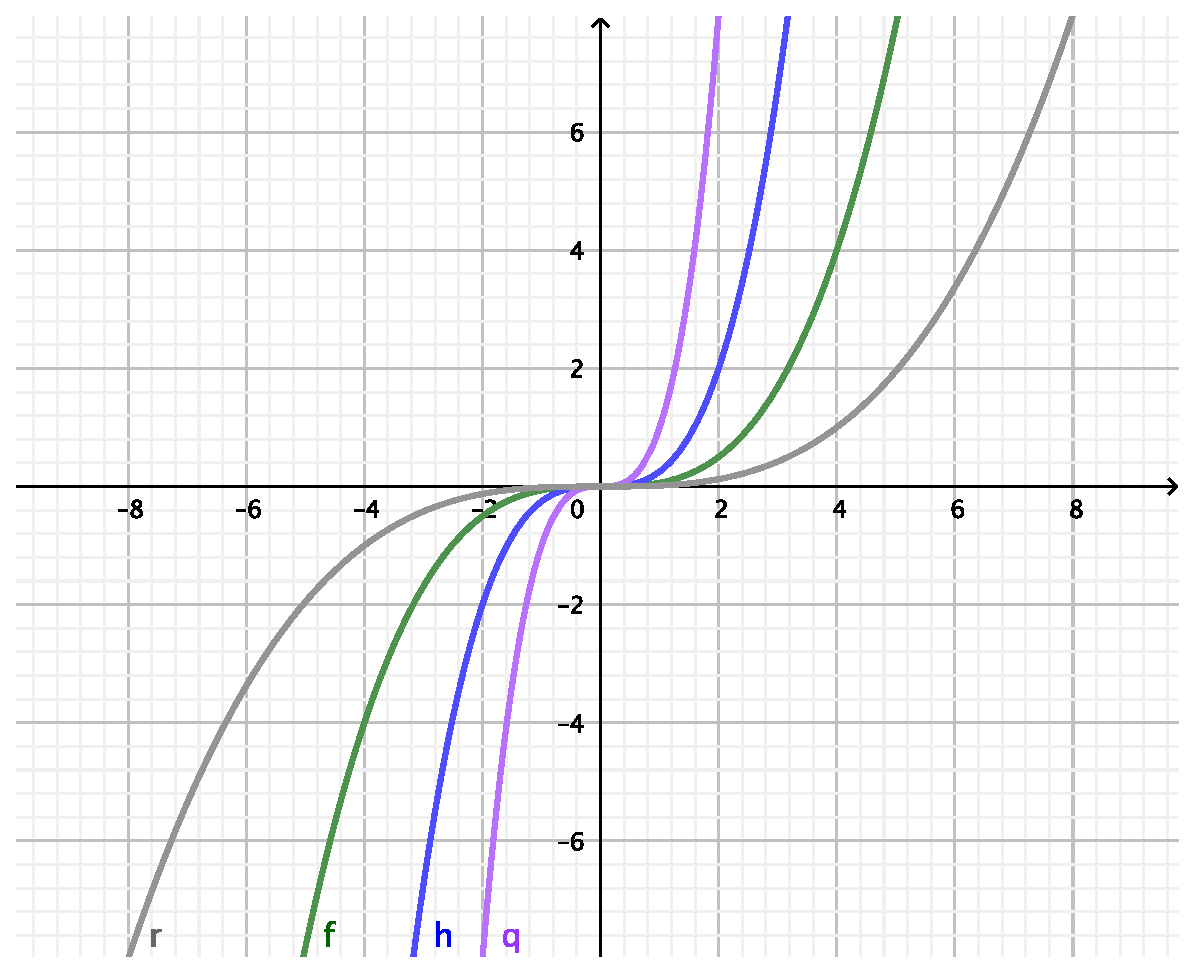
\includegraphics[height=12\baselineskip]{kap3/BundelFunktionenscharen.eps}
\end{minipage}

  \chapter{Trigonometrie}
\section{Kurze Wiederholung}
\begin{Definition}
  Im Kreis mit Radius 1 gelte:\\
  $\cos(\alpha)= x_{_M}$\\
  $\sin(\alpha)= y_{_M}$\\
  $\tan(\alpha)=\dfrac {sin(\alpha)} {cos(\alpha)}$
\end{Definition}\\
\definecolor{qqwuqq}{rgb}{0,0.39,0}
\definecolor{ttzzqq}{rgb}{0.2,0.6,0}
\definecolor{ffqqqq}{rgb}{1,0,0}
\definecolor{ttttff}{rgb}{0.2,0.2,1}
\definecolor{uququq}{rgb}{0.25,0.25,0.25}
\begin{tikzpicture}[line join=round,x=2.0833333333333335cm,y=2.0833333333333335cm]
  \draw[->,color=black] (-1.2,0) -- (1.2,0) node[below]{$x$};
  \foreach \x in {-1,1}
  \draw[shift={(\x,0)},color=black] (0pt,2pt) -- (0pt,-2pt) node[below] {\footnotesize $\x$};
  \draw[->,color=black] (0,-1.2) -- (0,1.2) node[left]{$y$};
  \foreach \y in {-1,1}
  \draw[shift={(0,\y)},color=black] (2pt,0pt) -- (-2pt,0pt) node[left] {\footnotesize $\y$};
  \draw[color=black] (0pt,-10pt) node[right] {\footnotesize $0$};
  \clip(-1.2,-1.2) rectangle (1.2,1.2);
  \draw [shift={(0,0)},color=qqwuqq,fill=qqwuqq,fill opacity=0.1] (0,0) -- (0:0.21) arc (0:57.13:0.21) -- cycle;
  \draw [line width=0.4pt] (0,0) circle (2.08cm);
  \draw (0,0)-- (0.54,0.84);
  \draw [line width=1.6pt,color=ttttff] (0,0.84)-- (0.54,0.84);
  \draw [line width=1.6pt,color=ffqqqq] (0.54,0.84)-- (0.54,0);
  \draw [line width=1.6pt,color=ttzzqq] (1,-1.2) -- (1,1.2);
  \begin{scriptsize}
    \fill [color=uququq] (0,0) circle (1.5pt);
    \draw[color=uququq] (-0.11,-0.11) node {$O$};
    \fill [color=black] (0.54,0.84) circle (1.5pt);
    \draw[color=black] (0.61,0.92) node {$M$};
    \fill [color=uququq] (0,0.84) circle (1.5pt);
    \draw[color=uququq] (0.03,0.94) node {$A$};
    \fill [color=uququq] (0.54,0) circle (1.5pt);
    \draw[color=uququq] (0.7,0.04) node {$B$};
    \draw[color=ttttff] (0.3,0.74) node {cos(α)};
    \draw[color=ffqqqq] (0.74,0.4) node {sin(α)};
    \draw[color=ttzzqq] (0.82,1.1) node {tan(α)};
    \draw[color=qqwuqq] (0.12,0.07) node {$\alpha$};
  \end{scriptsize}
\end{tikzpicture}
\\\\\\
Es ergeben sich folgende (wissenswerte) Werte:
\\
\begin{center}
  \begin{tabu}to 0.9\textwidth {|X[c]|X[c]|X[c]|X[c]|X[c]|X[c]|X[c]|X[c]|X[c]|}
    \hline
    & 0$^\circ$ & 30$^\circ$ & 45$^\circ$ & 60$^\circ$ & 90$^\circ$ & 180$^\circ$ & 270$^\circ$ & 360$^\circ$\\
    & 0 & $\dfrac{\pi}{6}$ & $\dfrac{\pi}{4}$ & $\dfrac{\pi}{3}$ & $\dfrac{\pi}{2}$ & \pi & $\dfrac{3\pi}{2}$ & 2\pi\\
    \hline
    $\sin(\alpha)$ & 0 & $\dfrac{1}{2}$ & $\dfrac{1}{\sqrt{2}}$ & $\dfrac{\sqrt{3}}{2}$ & 1 & 0 & -1 & 0\\
    \hline
    $\cos(\alpha)$ & 1 & $\dfrac{\sqrt{3}}{2}$ & $\dfrac{1}{\sqrt{2}}$ & $\dfrac{1}{2}$ & 0 & -1 & 0 & 1\\
    \hline
    $\tan(\alpha)$ & 0 & $\dfrac{{1}}{\sqrt{3}}$ & 1  & $\sqrt{3}$ & X & 0 & X & 0\\
    \hline
  \end{tabu}
\end{center}
\section{Addtions- und Verdopplungssätze}
\begin{Theorem}
  $\cos(a - b) = \cos(a)\cos(b) + \sin(a)\sin(b)$\\
  $\sin(a - b) = \sin(a)\cos(b) - \cos(a)\sin(b)$\\
  $\cos(a + b) = \cos(a)\cos(b) - \sin(a)\sin(b)$\\
  $\sin(a + b) = \sin(a)\cos(b) + \cos(a)\sin(b)$
\end{Theorem}
\\
Hieraus ergeben sich einige weitere Relationen, wie z.B. $\sin(2a)$. Diese lassen sich jedoch schnell und leicht herleiten.
\section{Allgemeine Sinus- und Kosinussätze}
In einem beliebigen Dreieck gelten abgewandelte Formen der aus der 8. Klasse bekannten Sätze:
\begin{Theorem}
  $\dfrac {a} {sin(\alpha)}=\dfrac {b} {sin(\beta)}=\dfrac {c} {sin(\gamma)}$\\\\
  $c²=a²+b²-2abcos(\gamma)$
\end{Theorem}
\definecolor{qqwuqq}{rgb}{0,0.39,0}
\begin{tikzpicture}[line cap=round,line join=round,>=triangle 45,x=0.53cm,y=0.64cm]
  \clip(-0.4,-4.3) rectangle (9,3);
  \draw [shift={(4.22,1.92)},color=qqwuqq,fill=qqwuqq,fill opacity=0.1] (0,0) -- (-134.14:1.5) arc (-134.14:-47.61:1.5) -- cycle;
  \draw [shift={(-0.38,-2.82)},color=qqwuqq,fill=qqwuqq,fill opacity=0.1] (0,0) -- (1.04:1.5) arc (1.04:45.86:1.5) -- cycle;
  \draw [shift={(8.4,-2.66)},color=qqwuqq,fill=qqwuqq,fill opacity=0.1] (0,0) -- (132.39:1.5) arc (132.39:181.04:1.5) -- cycle;
  \draw (4.22,1.92)-- (8.4,-2.66);
  \draw (4.22,1.92)-- (-0.38,-2.82);
  \draw (8.4,-2.66)-- (-0.38,-2.82);
  \begin{scriptsize}
    \draw[color=black] (6.7,-0.44) node {$a$};
    \draw[color=black] (1.76,-0.08) node {$b$};
    \draw[color=black] (4.06,-2.28) node {$c$};
    \draw[color=qqwuqq] (4.4,1.05) node {$\gamma$};
    \draw[color=qqwuqq] (0.7,-2.45) node {$\alpha$};
    \draw[color=qqwuqq] (7.5,-2.2) node {$\beta$};
  \end{scriptsize}
\end{tikzpicture}\\
Man bemerkt, dass sich die bekannten Relationen ergeben, wenn einer der Winkel den Wert $\dfrac{\pi}{2}$ annimmt.
\section{Sinusfunktionen}
Zur Vollständigen Funktionsdiskussion einer Sinus-Funktion sind einige Besonderheiten zu beachten:
\begin{enumerate}
  \item Amplitude und Periodizität\\
  Eine Funktion der Form $f(x)=a\cdot\sin(b(x-c))+d$ hat:
  \begin{itemize}
    \item die Periode $P = \dfrac{2\pi}{|b|}$
    \item die Amplitude $A = |a|$
    \item die Verschiebung entlang der $x$-Achse um $d$ und entlang der $y$-Achse um $c$
    \end{itemize}
  \item Symmetrieeigenschaften\\
  Hier sollte zumindest bekannt sein, dass $f(x)=\sin(x)$ punktsymmetrisch zum Origo ist, und dass $f(x)=\cos(x)$ Achsensymmetrisch zur $y$-Achse ist.
  \item Die Null-, Extrem- und Wendestellen sind in Form einer Menge anzugeben. (Es sei denn, die Aufgabenvorschrift fordert explizit auf eine Begrenzung auf ein angegebenes Intervall auf)\\
  Bsp: Die Nullstellen der Funktion $f(x)=\sin(x)$ lassen sich dartstellen als: $x \in \{k\pi|k \in \Z\}$
  \\ In umgebung einfärben
  \item Bei der Teilung durch eine Sinusfunktion können Definitionslücken an dessen Nullstellen entstehen. Auch diese können in der bereits gezeigten Form angegeben werden.
  \end{enumerate}
\section{Polarkoordinaten}
In der Kursstufe beschränken wir uns auf die Benutzung von Polarkoordinaten für Punkte in der Ebene (2D).
\begin{Definition}
  Polarkoordinaten sind eine Form der eindeutigen Punktangaben, doch anstatt wie kartesische Koordinaten 2 Entfernungen $x$ und $y$ zu verwenden, haben sie die Form $(r|\varphi)$. $r$ ist hierbei die Entfernung zum Origo und $\varphi$ ein orientierter Winkel (in $rad$).
\end{Definition}
\definecolor{zzzzzz}{rgb}{0.6,0.6,0.6}
\definecolor{ffqqqq}{rgb}{1,0,0}
\definecolor{qqzzqq}{rgb}{0,0.6,0}
\begin{tikzpicture}[line cap=round,line join=round,x=1.0cm,y=1.0cm]
  \draw[->,color=black] (-0.2,0) -- (2.64,0);
  \foreach \x in {,1,2}
  \draw[shift={(\x,0)},color=black] (0pt,-2pt);
  \draw[color=black] (2.47,0.04) node [anchor=south west] { x};
  \draw[->,color=black] (0,-0.29) -- (0,2.63);
  \draw[color=black] (0.05,2.43) node [anchor=west] { y};
  \clip(-0.2,-0.29) rectangle (2.64,2.63);
  \draw [shift={(0,0)},color=ffqqqq,fill=ffqqqq,fill opacity=0.1] (0,0) -- (0:0.41) arc (0:46.48:0.4) -- cycle;
  \draw [color=qqzzqq] (0,0)-- (2.05,2.16);
  \draw [color=zzzzzz] (0,2.16)-- (2.05,2.16);
  \draw [color=zzzzzz] (2.05,2.16)-- (2.05,0);
  \begin{scriptsize}
    \fill [color=black] (2.05,2.16) circle (1.5pt);
    \draw[color=black] (2.12,2.29) node {$P$};
    \draw[color=qqzzqq] (1.16,1.04) node {r};
    \draw[color=ffqqqq] (0.5,0.17) node {$\varphi$};
    \draw[color=zzzzzz] (0.96,2.02) node {y};
    \draw[color=zzzzzz] (1.9,1.03) node {x};
  \end{scriptsize}
\end{tikzpicture}
\subsection{Umrechnung}
\subsubsection{Kartesisch $\rightarrow$ Polar}
\begin{itemize}
  \item  $r=\sqrt{x^2+y^2}$
  \item $\varphi = \tan(\dfrac{y}{x})$
\end{itemize}
\subsubsection{Polar $\rightarrow$ Kartesisch}
\begin{itemize}
  \item $x = r\cdot\cos(\varphi)$
  \item  $y=r\cdot\sin(\varphi)$
\end{itemize}

  \chapter{Exponentialfunktionen}

\begin{Definition}
Man bezeichnet als Exponentialfunktion eine Funktion der Form $x\rightarrow a^x$ mit $a\in \R$, $a>0$ und $a\neq1$\\
$x$ ist die Variable und wird \textit{Exponent} oder \textit{Hochzahl} genannt.\\
$a$ nennt man \textit{Basis} oder \textit{Grundzahl}, sie ist für jede Funktion fest forgegeben.\\
Die natürliche Exponentialfunktion wird durch die Funktionsvorschrift $f(x)=e^x$ beschrieben.
\end{Definition}

Hier Graphen für a<1\\
a>1\\
a=e\\


		\section{Wiederholung: Potenzgesetze}
Seien $a$ und $b$ aus $\R$, sowie $n$ und $m$ aus $\N$, dann gilt:
\begin{enumerate}
\begin{minipage}{0.5\textwidth}
\item$a^0=1$ (für $a\neq 0$)
\item$a^1=a$
\item$a^n=\underbrace{a\cdot a\cdot ... \cdot a}_{n Mal}$
\item$a^m\cdot a^n=a^{m+n}$
\item$(a^n)^m=a^{n\cdot m}$
\end {minipage}
\begin{minipage}{0.5\textwidth}
\item$a^{-n}=\dfrac{1}{a^n}$
\item$\dfrac{a^n}{a^m}=a^{n-m}$
\item$(\dfrac{a}{b})^n=\dfrac{a^n}{b^n}$
\item $a^{\dfrac{1}{n}}=\sqrt[n]{a}$
\item$a^{\dfrac{m}{n}}=\sqrt[n]{a^m}$
\end {minipage}
\end{enumerate}

		\section{Die Eulersche Zahl ($e$)}

\begin{Definition}
$e = 2,71828182845904523536028747135266249775724709369995...$\\
\\
$e$ ist eine irrationale, transzendente und reelle Zahl, die die Basis des (natürlichen) Logarithmus und der (natürlichen) Exponentialfunktion ist.\\
Die Darstellung, der man am Häufigsten begegnet ist diese:
$e=\lim\limits_{n\to \infty}(1+\dfrac{1}{n})^n$
\end{Definition}
Benannt nach dem bekannten Mathematiker Leonhard Euler ist diese Zahl eine der wichtigsten Konstanten der Mathematik.
Sie ist die Basis des natürlichen Logarithmus und der natürlichen Exponentialfunktion. Diese (spezielle) Exponentialfunktion wird aufgrund dieser Beziehung zur Zahl $e$ häufig kurz $e$-Funktion genannt.
\begin{Definition}
  Eine reelle Zahl heißt (oder allgemeiner eine komplexe Zahl) transzendent,
  wenn sie nicht Nullstelle eines Polynoms mit ganzzahligen Koeffizienten ist.
  Andernfalls handelt es sich um eine algebraische Zahl. Jede reelle transzendente Zahl ist überdies irrational.
\end{Definition}

	\subsection{Verschiedene Darstellungen}

$e$ ist darstellbar bzw. ergibt sich durch:
\begin{itemize}
\item $\sum\limits_{k=0}^{\infty}\dfrac{1}{k!}$
\item $\lim\limits_{t\to \infty}(1+\dfrac{1}{t})^t;t\in\R$
\item $\lim\limits_{n\to \infty}(1+\dfrac{1}{n})^n;n\in\N$
\end{itemize}

	\subsection{Herleitung zur Zahl $e$}

Anhand mancher Überlegungen, denen wir jetzt nachgehen werden, lassen sich einige Eigenschaften der Eulerschen Zahl schließen.\\
\\ Wir definieren eine Folge $(e_{n})n\in\N$ durch $e_{n}=(1+\dfrac{1}{n})^n$ und versuchen ihre Konvergenz zu beweisen.
\begin{itemize}
\item$\dfrac{e_{n+1}}{e_{n}}=\dfrac{{(1+\dfrac{1}{n+1})}^{n+1}}{{(1+\dfrac{1}{n+1})}^{n}}=(\dfrac{n(n+2)}{(n+1)^2})^n\cdot(1+\dfrac{1}{n})=(1-\dfrac{1}{(n+1)^2})^{n+1}\cdot\dfrac{n+1}{n}$
\item Die Umformung ermöglicht uns auf den Term ${(1-\dfrac{1}{(n+1)^2}})^{n+1}$, die Ungleichung von Bernoulli anzuwenden. Diese besagt Folgendes: $(1+x)^n>1+nx$ für $n>gleich2$ und $x>-1$\\
$(1-\dfrac{1}{(n+1)^2})^{n+1}>1+(n+1)\cdot(-\dfrac{1}{(n+1)^2})$
\item Dies kann man an den ersten Ausdruck anwenden:\\
$\Rightarrow(1-\dfrac{1}{(n+1)^2})^{n+1}\cdot\dfrac{n+1}{n}>1+(n+1)\cdot(-\dfrac{1}{(n+1)^2})\cdot\dfrac{n+1}{n}=1-\dfrac{1}{n}$

\end{itemize}

		\section{Eigenschaften}
		\section{Ableitungsregeln}

\begin{enumerate}
\item 
\end{enumerate}
	\subsection{Aktivität}

Quelle: Déclic 1ère


  \documentclass[../MAIN/main.tex]{subfiles}
\begin{document}
\chapter{Logarithmen}
\chapterauthor{Clara}

\begin{Definition}
Der Logarithmus einer Zahl ist der Exponent, mit dem die Basis des Logarithmus' potenziert werden muss, um die gegebene Zahl zu erhalten. Logarithmen sind nur für positive reelle Zahlen definiert, die Basis muss positiv und ungleich $1$  sein
\begin{center}
$\log_ba=x\Leftrightarrow b^x=a$
\end{center}
\end{Definition}

\begin{Definition}
Man bezeichnet als Logarithmusfunktion eine Funktion der Form $x\rightarrow \log_bx$ mit $b\in \R^+\backslash 1$\\
$x$ ist die Variable und wird \textit{Argument} oder \textit{Numerus} genannt, Logarithmusfunktionen sind nur für positive, reelle Zahlen definiert: $x\in\R^+$\\
$b$ nennt man \textit{Basis} oder \textit{Grundzahl}, sie ist für jede Funktion fest forgegeben.\\
\end{Definition}

Hier Graphen
\subsubsection{Besondere Logarithmen}

$\begin{array}{lcccl}
\mbox{Logarithmus naturalis}&:&\ln a&:=&\log_ea\\
\mbox{Logarithmus dualis}&:&\ld a&:=&\log_2a\\
\mbox{Dekadischer Logarithmus}&:&\lg a&:=&\log_{10}a
\end{array}$
\\
	
			\section{Rechengesetze}

Aus den Potenzgesetzen kann man die Logarithmussätze erhalten.

\begin{Theorem}
Seien $a,b,c\in\R^+$ und $n\in\N$\\
\begin{center}
$\begin{array}{cccl}
\log_c(a\cdot b)&=&\log_ca+\log_cb&\qquad\mbox {Produktregel}\\
\log_c\left(\dfrac{a}{b}\right)&=&\log_ca-\log_cb&\qquad\mbox{Quotientenregel}\\
\log_ca^n&=&n\cdot\log_ca&\qquad\mbox{1. Potenzregel}\\
\log_c\sqrt[n]{a}&=&\dfrac{1}{n}\cdot\log_ca&\qquad\mbox{2. Potenzregel}\\
\end{array}$
\end{center}
\end{Theorem}

\begin{Bemerkung}
Die zweite Potenzregel ist nur ein Sonderfall der ersten, da $\sqrt[n]{a}=a^{\frac{1}{n}}$
\end{Bemerkung}

		\section{Gleichungen lösen}


\begin{Beispiel}
\begin{itemize}
\item $\ln(x-2)+\ln(x+2)=\ln(4+2x)\Leftrightarrow \ln\left(\dfrac{(x-2)\cdot (x+2)}{2\cdot (2+x)}\right)=0\Leftrightarrow \ln \left(\dfrac{x-2}{2}\right)=0\Leftrightarrow \dfrac{x-2}{2}=1\Leftrightarrow x=4$
\item $\ln (1-x) + \ln (1+x)=2(\ln3-\ln5)\Leftrightarrow \ln \left(\dfrac{(1-x)\cdot (1+x)\cdot 5^2 }{ 3^2}\right)=0\Leftrightarrow \dfrac{(1-x)\cdot (1+x)\cdot 5^2 }{ 3^2}=1\Leftrightarrow x=\pm  \dfrac{4}{5} $
\item$ e^{2+\ln x}=x+3\Leftrightarrow e^2 \cdot x=x+3\Leftrightarrow x=\dfrac{3}{e^2-1}$
\item $2x\ln (3e^x-2)\Leftrightarrow$
\end{itemize}
\end{Beispiel}


		\section{Logarithmusfunktionen}


	\subsection{Eigenschaften}

\begin{itemize}
\item$f(x)=\log_bx$
\item$b\in\R^+\backslash 1$
\item$D_f=\R^+$
\item$W_f=\R$
\item für $0>b>1$: $f$ ist streng monoton wachsend\\
für $b>1$: $f$ ist streng monoton fallend
\item für $0>b>1$: $\lim\limits_{x\to +\infty}f(x)=-\infty$\\
			$\lim\limits_{x\to 0}f(x)=+\infty$\\
für $b>1$: $\lim\limits_{x\to +\infty}f(x)=+\infty$\\
	        $\lim\limits_{x\to 0}f(x)=-\infty$
\item $f(1)=0$
\item y-Achse ist senkrechte Asmyptote
\end{itemize}


	\subsection{Ableitungsregeln}
	\subsection{Funktionsuntersuchungsbeispiel}
\end{document}

  \chapter{Integrale}
\section{Stammfunktionen}
Eine Funktion $F$ heißt Stammfunktion der Funktion $f$, wenn $F'(x)=f(x)$
gilt.

Ist $F$ irgendeine Stammfunktion von $f$, dann ist auch $F(x)+C$ (mit
konstantem $C$) eine Stammfunktion, denn beim Ableiten fällt ja $C$ als
konstanter Summand weg. Jede Funktion hat also unendlich viele
Stammfunktionen, die sich aber nur um einen konstanten Summanden
unterscheiden.

\section{Begriff des Integrals}

\begin{figure}[htbp]\centering
  \includegraphics{math3.eps}
  \caption{Integral und Flächeninhalt}
  \label{fig:6}
\end{figure}

In Abb.~\ref{fig:6} soll die Fläche zwischen der x-Achse und der Funktion
$y=f(x)$ zwischen $x=a$ und $x=b$ berechnet werden.

Um eine Näherung für diese Fläche zu bekommen, teilt man sie in Streifen auf
(in der Abb.~\ref{fig:6} sind es 6 Streifen) und nimmt die Summe der
Flächeninhalte der Rechtecke als Näherung für die Fläche. Wenn man die Zahl
der Streifen so erhöht, dass die Breite jedes Streifens gegen Null geht, dann
bekommt man als Grenzwert die gesuchte Fläche. In Abb.~\ref{fig:6} ist die
Näherung:
\[
A_6=y_1(x_1-x_0)+y_2(x_2-x_1)+y_3(x_3-x_2)
+y_4(x_4-x_3)+y_5(x_5-x_4)+y_6(x_6-x_5)
\]
Beachtet man, dass $y_k=f(x_k)$ ist und schreibt man $\Delta x_1=x_1-x_0$,
$\Delta x_2=x_2-x_1$ usw., dann bekommt man für $n$ Streifen:
\[
A_n=f(x_1)\Delta x_1+f(x_2)\Delta x_2+\cdots+f(x_n)\Delta x_n=
\sum_{k=1}^n f(x_k)\Delta x_k
\]

Der Grenzwert dieser $A_n$ ist nun die gesuchte Fläche:
\begin{equation}
  \label{eq:33}
  \int_a^b \dD y=
  \int_a^b f(x)\dD x=\lim_{n\to\infty}\sum_{k=1}^n f(x_k)\Delta x_k
\end{equation}
Beim Grenzübergang ist nur zu beachten, dass mit Erhöhung der Streifenzahl $n$
auch alle Breiten $\Delta x_k$ gegen Null gehen, also
$\lim_{n\to\infty}\max\Delta x_k=0$ gilt.

Schaut man sich die Abb.~\ref{fig:6} an, dann stellt man fest, dass statt
$f(x_k)$ als Seite der Rechtecke auch Rechtecke verwendet werden könnten,
deren Seite irgendein $f(u_k)$ ist, wobei $x_{k-1}\le u_k\le x_k$ ist.

Grenzwerte der Art von Gl.~\eqref{eq:33} heißen \emph{Integrale}. Funktionen,
für die dieser Grenzwert für jede Art der Unterteilungsfolge und jede Wahl der
$f(u_k)$ existiert und immer denselben Wert ergibt, heißen \emph{integrierbar}.

Als Physiker sagt man, durch Integration werden Elemente der Form  $\dD
y=f(x)\dD x$
aufaddiert.

\section[Der Hauptsatz]{Der Hauptsatz der Differential- und
  Integralrechnung}
Die Bestimmung der Grenzwerte in Gleichung~\eqref{eq:33} ist eine mühselige
Angelegenheit. Aber alles wendet sich zum Guten, denn Integrale können mittels
Stammfunktionen bestimmt werden.

Um dies klar zu machen betrachten wir irgendeine Stammfunktion $F$ der
Randfunktion $f$. Nach der Grundformel~\eqref{eq:34} ist dann
\[
\dD F(x)=F'(x)\dD x=f(x)\dD x\Rpf
\Delta F(x_k)\approx f(x_k)\Delta x_k\Rpf
F(x_k)-F(x_{k-1})\approx f(x_k)\Delta x_k
\]
Die Näherung ist umso besser je kleiner $\Delta x_k$ ist.

Wendet man diese Beziehung auf die Näherungssumme $A_n$ an, dann bekommt man:
\[
A_n\approx(F(x_1)-F(x_0))+(F(x_2)-F(x_1))+\cdots (F(x_n)-F(x_{n-1})
\]
In dieser Gleichung heben sich alle Summanden bis auf $F(x_0)$ und $F(x_n)$
heraus, also ist, weil $x_0=a$ und $x_n=b$ ist, $A_n\approx F(b)-F(a)$.

Diese Näherung wird umso besser, je kleiner die $\Delta x$ werden, also hat
man für den Grenzwert:
\begin{merkbox}
\begin{equation}
  \label{eq:35}
  \int_a^b f(x)\dD x
  =\lim_{n\to\infty}\sum_{k=1}^n f(x_k)\Delta x_k = F(b) - F(a)
  =\left[F(x)\right]_a^b
\end{equation}
\end{merkbox}
Dies ist der \textbf{Hauptsatz der Differential- und Integralrechnung}. Mit
ihm wird das Problem der Integration auf das Auf"|finden einer Stammfunktion
zurückgeführt. Als Mathematiker müsste man noch anfügen, dass diese Beziehung
nicht immer gilt, sondern nur unter gewissen Voraussetzungen.

Der Hauptsatz ist sicher dann richtig, wenn die Funktion $f$ stetig ist.
In diesem Fall kann man auch so formulieren:
\[
I_a(x)=\int_a^x f(\xi)\dD \xi \qquad\Rpf\qquad I_a'(x)=f(x)
\]
Die Funktion $I_a$ nennt man hier die Integralfunktion. Man kann sie sich
vorstellen als die Funktion die jeder Stelle $x$ die Fläche zwischen $a$ und
$x$ zuordnet. Unter den obigen Voraussetzungen ist also die Ableitung der
Integralfunktion gleich der Randfunktion. Ist die Randfunktion $f$ nicht im
ganzen Intervall stetig, sondern nur ">stückweise stetig"<, dann ist zwar die
Integralfunktion immer noch stetig, aber in den Trennpunkten der
Stetigkeitsbereiche nicht mehr notwendig differenzierbar.

Häufig kommen auch sogenannte \emph{unbestimmte Integrale} vor. Ein
unbestimmtes Integral ist einfach eine Stammfunktion. Man schreibt dann
\[
\int f(x)\dD x= F(x)+C
\]
und nennt $C$ die \emph{Integrationskonstante}.

Eine Stammfunktion zu finden, ist allerdings häufig auch nicht sehr einfach.
Für viele aus elementaren Funktionen zusammengesetzte Funktionen bekommt man
leider Stammfunktionen, die nicht mehr elementar dargestellt werden können. Das gilt
schon für so einfach aussehende Integrale wie
\[
\int \frac{\sin x}{x}\dD x
\]

Da $\sin x /x$ in ihrem Definitionsbereich stetig ist, muss sie nach dem
Hauptsatz eine Stammfunktion haben. Sie lässt sich allerdings nicht mehr durch
elementare Funktionen ausdrücken, sondern gibt eine ">neue"< sogenannte
">höhere"< Funktion, die man Integralsinus nennt. Ihre Funktionswerte kann man
mit Tabellen oder mit Computerprogrammen bestimmen. Zunächst mag man meinen,
dies sei etwas besonderes, aber auch die Werte eines Logarithmus oder eines
Sinus kann man nur mit dem Taschenrechner berechnen oder aus einer
Funktionentafel entnehmen.

\section{Integrationsregeln}

Da Integration die Umkehrung des Ableitens ist (">Aufleiten"<) übertragen sich
die Ableitungsregeln auf das Integrieren:
\begin{itemize}
\item Konstante Faktoren bleiben stehen.
\item Summen werden summandenweise aufgeleitet.
\item $\D\int_a^b=\int_a^c+\int_c^b$
\item $\D \int_a^b=-\int_b^a$
\item Es gibt \emph{keine direkte} Umkehrung der Produkt-, Quotienten und
  Kettenregel, sondern hier muss man kompliziertere Verfahren verwenden.
\end{itemize}

Wichtige Integrale sind:
\begin{align}
  \label{eq:36}
  \int x^n\dD x&=\frac{x^{n+1}}{n+1}\\
  \int\sin x\dD x&= -\cos x\label{eq:37}\\
  \int\cos x\dD x&= \sin x\label{eq:38}\\
  \int\frac{\dD x}{\cos^2x}&= \tan x\label{eq:39}\\
  \int\frac{1}{x}\dD x&= \ln|x|\label{eq:40}\\
  \int\frac{\dD x}{1+x^2}&= \arctan x\label{eq:41}
\end{align}

In Formelsammlungen stehen viele Integrale, es gibt auch Integraltafeln, die
hunderte von Integralen fertig angeben. CAS-Programme können alle sehr gut
integrieren.

Aus der Formel~\eqref{eq:35} erkennt man, dass das Integral negativ wird, wenn
im betrachteten Intervall $f(x)<0$ ist. Dann verläuft die Kurve unterhalb der
x-Achse, und man muss als Fläche den Betrag nehmen. Integrale sind aber nicht
nur Flächen, mit ihnen kann man Volumina, Energien, Ladungen und und und
\ldots ausrechnen, und bei vielen dieser Größen sind negative Werte durchaus
sinnvoll!

\subsection{Produktintegration}
Nach der Produktregel ist $(uv)'=u'v+uv'$. Integriert man nun beide Seiten,
und beachtet, dass nach dem Hauptsatz $\int (uv)'\dD x=uv$ ist, dann bekommt
man die Formel für die Produktintegration, die auch \emph{partielle
  Integration} genannt wird.
\begin{equation}
  \label{eq:42}
  \int u'v\dD x= uv - \int uv'\dD x
\end{equation}

Mit dieser Regel kann man \zB Integrale folgender Form lösen:
\[
\int x\sin x\dD x
\]
Setzt man hier $u'=\sin x$, $v=x$, dann ist $u=-\cos x$ und $v'=1$. Setzt man
diese Werte in die Produktintegrations-Formel ein, dann folgt:
\begin{align*}
\int x\sin x\dD x&= (-\cos x)x-\int (-\cos x)\cdot1\dD x\\
&=-x\cos x+\int\cos x\dD x= -x\cos x+\sin x
\end{align*}

Ein anderes schönes Beispiel ist die Stammfunktion von $\ln x$. Dazu fasst man
$\ln x$ als $1\cdot\ln x$ auf und wählt $u'=1$, $v=\ln x$, also $u=x$ und
$v'=1/x$ und erhält:
\[
\int\ln x\dD x=x\ln x-\int x\cdot\frac{1}{x}\dD x=
x\ln x-\int 1\dD x=x\ln x -x
\]

\subsection{Substitutionsmethode}
Es soll die Stammfunktion von $x(1-x^2)^9$ bestimmt werden. Hier wäre zum
Ableiten die Kettenregel und die Produktregel nötig, beides gibt es aber in
reiner Form beim Integrieren nicht. Man kann aber häufig durch geschickte
Substitution das Integral auf eine Form bringen, für die dann eine
Stammfunktion angegeben werden kann. Der wesentliche Punkt dabei ist, dass
nicht nur $x$ sondern auch $\dD x$ der Substitution unterworfen werden muss.

In diesem Beispiel setzen wir $u=1-x^2$. Dann ist $\dD u=u'(x)\dD x=-2x\dD x$.
Somit ist $\dD x=-\dD u/2x$. Nun geht's los:
\[
\int x(1-x^2)^9\dD x=\int x u^9 \frac{-1}{2x}\dD u
=-\frac{1}{2}\int u^9\dD u=-\frac{1}{20}u^{10}=-\frac{1}{20}(1-x^2)^{10}
\]

Hätten wir hier die Stammfunktion nicht benötigt, sondern nur den Wert eines
bestimmten Integrals, dann hätte man sich die Rücksetzung sparen können, indem
man die Grenzen auf die neue Variable umschreibt:
\[
\int_{x=0}^1 x(1-x^2)^9\dD x=-\frac{1}{2}\int_{u=1}^0u^9\dD u
=-\frac{1}{20}\left[u^{10}\right]_1^0=-\frac{1}{20}(0-1)=\frac{1}{20}
\]

In diesem Beispiel haben wir einen Teilausdruck des Integrals gleich $u$
gesetzt. Im folgenden Beispiel machen wir es anders herum und setzen $x$
gleich einer Funktion von $u$. Es soll die Fläche einer Ellipse berechnet
werden. Für den oberen Ellipsenbogen gilt die Gleichung (Auflösen der
Mittelpunktsform~\eqref{eq:7} nach $y$):
\[
y=\frac{b}{a}\sqrt{a^2-x^2}
\]
Die Fläche unter dem oberen Ellipsenbogen ist die halbe Ellipsenfläche und
berechnet sich so:
\[
A=\int\limits_{x=-a}^a \frac{b}{a}\sqrt{a^2-x^2}\,\dD x=
\int\limits_{u=-\frac{\pi}{2}}^{\frac{\pi}{2}}
\frac{b}{a}\sqrt{a^2-a^2\sin^2u}\,a\cos u\,\dD u=
\int\limits_{-\frac{\pi}{2}}^{\frac{\pi}{2}}ab\cos^2u\,\dD u
\]
Dabei hat man $x=a\sin u$ gesetzt, dann wird $\dD x=a\cos u \dD u$. Nun muss
man nur noch die Stammfunktion von $\cos^2u$ ermitteln. Dazu kann man etwa die
Beziehung $\cos2u=2\cos^2u-1$ heranziehen, also
$\cos^2u=\frac{1}{2}(1+\cos2u)$. Diese hat die Stammfunktion
$\frac{1}{2}(u+\sin u\cos u)$. Damit bekommt man für die Fläche:
\[
A=\frac{ab}{2}\left[u+\sin u\cos u\right]_{-\frac{\pi}{2}}^{+\frac{\pi}{2}}=
\frac{ab}{2}[(\frac{\pi}{2}+0)-(-\frac{\pi}{2}+0)]=\frac{1}{2}\pi a b
\]
Die gesamte Fläche der Ellipse ist doppelt so groß, also $\pi a b$.

\subsection{Partialbruchzerlegung}
Die Partialbruchzerlegung ist ein allgemeines Verfahren zur Integration
gebrochen rationaler Funktionen. Es sei gegeben:
\begin{equation}
  \label{eq:68}
  f(x)=\frac{P(x)}{Q(x)}
  =\frac{a_0+a_1x+\dots+a_nx^n}{b_0+b_1x+\dots+b_mx^m}
\end{equation}
Im Falle $m\le n$ führt man zuerst eine Polynomdivision aus, dann bekommt man
eine ganzrationale Funktion und eine gebrochen rationale mit $m>n$, so dass
wir uns für das Weitere auf den Fall $m>n$ beschränken können.

Das Nennerpolynom kann im Komplexen vollständig in Linearfaktoren zerlegt
werden, im Reellen bleiben ggf. quadratische Faktoren übrig, die keine reellen
Nullstellen mehr haben. Seien nun $x_k$ die Nullstellen von $Q(x)$ mit der
Vielfachheit $\nu_k$ dann kann man $Q(x)$ stets auf die folgende Form bringen:
\begin{equation}
  \label{eq:69}
  Q(x)=b_m(x-x_1)^{\nu_1}(x-x_2)^{\nu_2}\dots(x-x_k)^{\nu_k}
  (x^2+\alpha_1x+\beta_1)^{\mu_1}\dots(x^2+\alpha_rx+\beta_r)^{\mu_r}
\end{equation}
Die gebrochen rationale Funktion $f(x)$ lässt sich nun als Summe von
Partialbrüchen schreiben. Dabei gilt:
\begin{enumerate}
\item Jeder Linearfaktor $(x-x_k)$ der Vielfachheit $\nu_k$ trägt zur
  Zerlegung die folgenden Summanden bei:
  \[
  \frac{A_1}{(x-x_k)}+\frac{A_2}{(x-x_k)^2}+\dots
  +\frac{A_{\nu_k}}{(x-x_k)^{\nu_k}}
  \]
\item Jeder quadratische Faktor mit der Vielfachheit $\mu_k$ trägt die
  folgenden Summanden bei:
  \[
  \frac{C_1x+D_1}{(x^2+\alpha x+\beta)}+
  \frac{C_2x+D_2}{(x^2+\alpha x+\beta)^2}+\dots+
  \frac{C_{\mu_k}x+D_{\mu_k}}{(x^2+\alpha x+\beta)^{\mu_k}}
  \]
\end{enumerate}

\noindent Die Linearfaktoren lassen sich sofort integrieren, bei den
quadratischen geht man so vor:
\[
(x^2+\alpha x+\beta)=\bigl(x+\tfrac{\alpha}{2}\bigr)^2+\delta^2
=(\delta y)^2+\delta^2=\delta^2(y^2+1)
\]
Hier hat man quadratisch ergänzt und $\delta\cdot y=x+\frac{\alpha}{2}$
substituiert. Mit dieser Substitution ist
\[
x=\delta y-\frac{\alpha}{2}\qquad y=\frac{x+\frac{\alpha}{2}}{\delta}\qquad
\dD x=\delta\dD y
\]
Nun wird das Integral zu:
\begin{align*}
  \int\frac{Cx+D}{(x^2+\alpha x+\beta)^\mu}\dD x
  &=\frac{1}{\delta^{2\mu-1}}
  \int\frac{C\delta y+D-\frac12C\alpha}{(y^2+1)^\mu}\dD y\\
  &=\frac{C}{\delta^{2\mu-2}}\int\frac{y\dD y}{(y^2+1)^\mu}
  +\frac{D-\frac12C\alpha}{\delta^{2\mu-1}}\int\frac{\dD y}{(y^2+1)^\mu}
\end{align*}
Für das erste der beiden verbleibenden Integrale bekommt man dann
\begin{equation}
  \label{eq:70}
  \int\frac{y\dD y}{(y^2+1)^\mu}=\frac12\int\frac{\dD u}{u^\mu}=
  \begin{cases}
    \dfrac{u^{1-\mu}}{2(1-\mu)}=&\text{für~}\mu=2, 3, \dots\\
    \frac{1}{2}\ln|u|& \text{für~} \mu=1
  \end{cases}
\end{equation}
Hier hat man $u=y^2+1$ gesetzt. Nun muss noch das zweite bestimmt werden.
\[
J_\mu=\int\frac{\dD y}{(y^2+1)^\mu}
\]
Für $\mu=1$ ist es bekannt, $J_1=\arctan y$.

Wir werden eine Rekursionsformel für die $J_\mu$ herleiten. Wir beginnen mit
der Beziehung
\[
J_{\mu+1}=\int\frac{(y^2+1)-y^2}{(y^2+1)^{\mu+1}}\dD y
=J_\mu-\int\frac{y^2}{(y^2+1)^{\mu+1}}\dD y
\]
Nun denken wir uns den zweiten Integranden als $y\cdot$Rest geschrieben und
integrieren partiell:
\[
\int y\cdot\frac{y\dD y}{(y^2+1)^{\mu+1}}=
\frac{-y}{2\mu(y^2+1)^\mu}+\frac{1}{2\mu}\int\frac{\dD y}{(y^2+1)^\mu}=
\frac{-y}{2\mu(y^2+1)^\mu}+\frac{1}{2\mu}\,J_\mu
\]
Setzt man das oben ein, so bekommt man die Rekursionsformel:
\begin{equation}
  \label{eq:71}
  J_{\mu+1}=\left(1-\frac{1}{2\mu}\right)J_\mu+\frac{y}{2\mu(y^2+1)^\mu}
\end{equation}
Insbesondere ist dann (rechne das nach!)
\begin{align*}
  J_1&=\arctan y\\
  J_2&=\frac{1}{2}\arctan y+\frac{y}{2(y^2+1)}\\
  J_3&=\frac38\left(\arctan y+\frac{y}{y^2+1}\right)+\frac{y}{4(y^2+1)^2}\\
  J_4&=\frac{5}{16}\left(\arctan y+\frac{y}{y^2+1}\right)+
       \frac{5}{24}\cdot\frac{y}{(y^2+1)^2}+\frac{y}{6(y^2+1)^3}
\end{align*}

\section{Beispiele zur Integration}
\NA Man bestimme die Fläche unter der Parabel $y=2x^2$ im Bereich $1\le x\le
4$.
\[
\int_1^4 2x^2\dD x=\left[\frac{2}{3}x^3\right]_1^4=\frac{2}{3}(64-1)=42
\]

\NA Bestimme die Formel für das Volumen einer Pyramide der Höhe $h$ und der
Grundfläche $G$.

Man stellt sich die Pyramide aus dünnen Schichten der Dicke $\dD x$ parallel
zur Grundfläche aufgebaut vor. Die x-Achse legt man durch die Spitze der
Pyramide, so dass die Höhe auf die x-Achse zu liegen kommt. Da die Flächen der
Schichten dann durch zentrische Streckung aus der Grundfläche entstehen, hat
eine Schicht im Abstand $x$ von der Spitze die Fläche $A(x)$, für die nach dem
Strahlensatz gilt:
\[
\frac{x^2}{h^2}=\frac{A(x)}{G}\quad\Rpf\quad A(x)=\frac{G}{h^2} x^2
\]
Das Volumen einer Schicht ist dann $\dD V=A(x)\dD x$. Das Volumen der Pyramide
ist die Summe der Volumina aller Schichten, diese Summe bekommt man durch
Integration:
\[
V=\int_0^h \dD V=\int_0^h \frac{G}{h^2}x^2\dD x
=\frac{G}{h^2}\cdot\frac{1}{3}\left[x^3\right]_0^h=
\frac{G}{3h^2}(h^3-0)=\frac{1}{3}Gh
\]

\NA Bestimme die Energie, die notwendig ist, um einen Körper der Masse $m$ im
Schwerefeld der Masse $M$ vom Abstand $R$ ins Unendliche zu bringen.

Um den Körper das Stückchen $\dD r$ vom Zentralkörper zu entfernen, braucht
man die Arbeit $\dD W=F\dD r$, wobei $F$ die Gravitationskraft ist. Die gesamte
notwendige Arbeit ist dann:
\[
W=\int_R^{\infty}\dD W=\int_R^{\infty}G\frac{Mm}{r^2}\dD r=
GMm\left[-\frac{1}{r}\right]_R^{\infty}=GMm(0-(-\frac{1}{R}))=\frac{GMm}{R}
\]

Dies war ein Beispiel eines sogenannten \emph{uneigentlichen Integrals}, bei
solchen liegen entweder die Grenzen im Unendlichen, oder die Funktion selbst
wird an einer Stelle unendlich.

\NA Bestimme $ \D\int_{-\infty}^{\infty}\E^{-x^2}\dD x$

Diese Aufgabe habe ich eingefügt, weil das ein wichtiges Integral ist. Seine
Berechnung ist aber nicht ganz einfach, man muss einen ">Umweg"< machen.
Zuerst schreiben wir:
\[
\int_{-\infty}^{\infty}\E^{-x^2}\dD x=
\sqrt{\left(\int_{-\infty}^{\infty}\E^{-x^2}\dD x\right)
  \left(\int_{-\infty}^{\infty}\E^{-y^2}\dD y\right)}=
\sqrt{\int_{-\infty}^{\infty}\int_{-\infty}^{\infty}
    \E^{-(x^2+y^2)}\dD x\dD y}
\]
Führt man nun Polarkoordinaten ein, also $x=r\cos\phi; y=r\sin\phi$, dann ist
das Flächenelement $r\dD\phi\dD r$ und $x^2+y^2=r^2$. Das letzte Integral wird
dadurch
\[
\int_0^{2\pi}\dD\phi\int_0^{\infty}r\E^{-r^2}\dD r
=2\pi\left[-\tfrac12\E^{-r^2}\right]_0^{\infty}=\pi \qRpf
\int_{-\infty}^{\infty}\E^{-x^2}\dD x=\sqrt{\pi}
\]

Mit Substitution kann man nun noch beweisen:
\[
\int_{-\infty}^{\infty}\E^{-a x^2}\dD x=\sqrt{\frac{\pi}{a}}
\]
Dazu setzt man $u^2=ax^2\Rpf\dD u=\sqrt{a}\dD x$. Dies kann nur gehen, wenn
$a>0$ ist. Man kann zeigen, dass die Formel sogar für komplexe $a$ stimmt,
sofern $\Re a>0$ ist.

\paragraph{Anmerkung:} $\E^{-x^2}$ hat keine elementare Stammfunktion, es gibt
aber eine Reihe von höheren Funktionen, die mit diesem Integral verwandt sind.
Zunächst ist dabei die aus der Wahrscheinlichkeitsrechnung bekannte
Normalverteilung (\caps{Gau"s}-Verteilung) zu erwähnen, die durch
\[
\Phi(x)=\frac{1}{\sqrt{2\pi}}\int_{-\infty}^x\E^{-\frac{1}{2}t^2}\dD t
\qqbox{mit}\Phi(\infty)=1
\]
definiert ist. Daneben gibt es die \caps{Gau"s}sche Fehlerfunktion
\[
\textrm{erf}\,(x)=\frac{2}{\sqrt{\pi}}\int_0^x\E^{-t^2}\dD t\qqbox{wobei}
\Phi(x)=\frac{1}{2}\biggl(1+\textrm{erf}\,\Bigl(\frac{x}{\sqrt{2}}\Bigr)\biggr)
\]

\NA Bestimme das Integral durch Partialbruchzerlegung.
Es sei gegeben:
\[
f(x)=\frac{x+2}{(x^2-1)(x^2+1)^2}=\frac{A}{x-1}+\frac{B}{x+1}+
\frac{Cx+D}{(x^2+1)^2}+\frac{Ex+F}{x^2+1}
\]
Nun müssen die Koeffizienten $A,\dots,F$ bestimmt werden. Dazu multipliziert
man zuerst mit dem Hauptnenner durch:
\[
x+2=A(x+1)(x^2+1)^2+B(x-1)(x^2+1)^2+(Cx+D)(x^2-1)+(Ex+F)(x^4-1)
\]
Zunächst kann man nun für $x$ spezielle Werte einsetzen, so dass möglichst
viele Ausdrücke Null werden:
\begin{align*}
  x=1: &&& 3=8A \qRpf A=\tfrac{3}{8}\\
  x=-1:&&& 1=-8B \qRpf B=-\tfrac{1}{8}\\
  x=0: &&& 2=\tfrac38+\tfrac18-D-F
\end{align*}
Hätte man nur einfache Vielfachheiten, so könnte man auf diese Weise alle
Koeffizienten bestimmen. Hier ist das leider nicht der Fall, so dass wir zur
">Ochsentour"< greifen müssen. Dazu wird die rechte Seite ausmultipliziert und
dann ein Koeffizientenvergleich gemacht:
\begin{gather*}
  x+2=(A-B-D-F)+(A+B-C-E)x+(2A-2B+D)x^2\\
  \phantom{x}+(2A+2B+C)x^3+(A-B+F)x^4+(A+B+E)x^5
\end{gather*}
Der Koeffizientenvergleich liefert nun ein Gleichungssystem (wobei wir unsere
schon bekannten Werte für $A$ und $B$ gleich einsetzen)
\begin{align*}
  2&=\tfrac{3}{8}+\tfrac{1}{8}-D-F\\
  1&=\tfrac{3}{8}-\tfrac{1}{8}-C-E\\
  0&=\tfrac{3}{4}+\tfrac{1}{4}+D\qRpf D=-1\\
  0&=\tfrac{3}{4}-\tfrac{1}{4}+C\qRpf C=-\tfrac{1}{2}\\
  0&=\tfrac{3}{8}+\tfrac{1}{8}+F\qRpf F=-\tfrac{1}{2}\\
  0&=\tfrac{3}{8}-\tfrac{1}{8}+E\qRpf E=-\tfrac{1}{4}
\end{align*}
Setzt man die sich aus den letzten vier Gleichungen ergebenden Werte nun in die
beiden ersten ein, so sind diese erfüllt. Wir sind fertig und haben das
Ergebnis
\[
f(x)=\frac{\frac38}{(x-1)}-\frac{\frac18}{x+1}-\frac{\frac12x+1}{(x^2+1)^2}
-\frac{\frac14x+\frac12}{x^2+1}
\]
Nach den Gleichungen~\eqref{eq:70} und \eqref{eq:71} ergibt sich so:
\begin{gather*}
\int f(x)\dD x=\frac{3}{8}\ln|x-1|-\frac18\ln|x+1|+\frac14\cdot\frac{1}{x^2+1}\\
\phantom{x}-\frac12\arctan x-\frac{x}{2(x^2+1)}-\frac{1}{8}\ln|x^2+1|
-\frac12\arctan x
\end{gather*}

Der Koeffizientenvergleich ist deshalb so leicht gegangen, weil wir schon
einige Werte mit der Einsetze-Methode ermittelt hatten. Man hätte statt des
Koeffizientenvergleichs auch weitere Gleichungen erzeugen können, indem man
einfach weitere Zahlen einsetzt. Wenn irgend möglich, sollte man versuchen mit
der Einsetze-Methode zum Ziel zu kommen. Am aller einfachsten ist es
allerdings, Mathematica anzuwerfen, dann hat man das Integral in
Sekundenbruchteilen.

  \chapter{Vektorielle Geometrie}


\section{Vektoren}
    \begin{Definition}
        Ein Vektor ist Element eines Vektorraums.
    \end{Definition}\\
    \paragraph{} Vektorräume, wir erinnern uns zurück. Verknüpfungen, inverse Elemente und die dazugehörenden Gesetze, konsequente Definitionen und mathematische Korrektheit, die guten alten Zeiten...\\
    Tatsächlich kann ein Vektor in den meisten Fällen als Verschiebung bezeichnet werden, \textbf{nicht aber als Pfeil oder Strich!}\\

    \subsection{Besondere Vektoren}

        \subsubsection{Der Ortsvektor}

            \paragraph{} Der Vektor von $O$ auf den Punkt $P$, geschrieben als $\vv{OP}$ oder $\vv{o}$.\\
            \paragraph{} Hat $P$ die Koordinaten $(P_1|P_2|...|P_n)$, so besitzt $\vv{o}$ die Darstellung $\left(\begin{array}{c} P_1 \\ P_2 \\ ...\\P_n\end{array}\right)$.

        \subsubsection{Der Nullvektor}

            \paragraph{} Der Vektor mit Wert $\left(\begin{array}{c} 0 \\ 0 \\ ...\\0\end{array}\right)$, er hat keine und alle Richtungen zugleich.
            \begin{Bemerkung}
                Er ist somit das neutrale Element der Vektoraddition.
            \end{Bemerkung}

        \subsubsection{Der Verbindungsvektor}

            \paragraph{} Der Vektor $\vv{AB}$ ist der Vektor, der den Punkt $A$ auf den Punkt $B$ abbildet. Er ist definiert als:\\ $\vv{AB}=\vv{OB}-\vv{OA}$, woraus folgt, dass: \begin{center} $\vv{AB} = \left(\begin{array}{c} b_1 - a_1 \\ b_2 - a_2 \\ ... \\ b_n - a_n \end{array}\right)$. \end{center}

        \subsubsection{Der Gegenvektor}

            \paragraph{} Der Gegenvektor zu $\vv{AB}$ ist $\vv{BA}$, definiert als  $-\vv{AB}$.
            \begin{Bemerkung}
                Er ist somit das inverse Element der Vektoraddition.
            \end{Bemerkung}

    \subsubsection{Der Einheitsvektor}

        \subsubsubsection{Norm eines Vektors}

            \paragraph{} Die Norm eines Vektors ist anschaulich als seine Länge zu interpretieren. Der Betrag, wie sie ebenfalls genannt wird, eines Vektors $\vv{v}$ ist folgendermaßen definiert: $\text{|}\vv{v}\text{|} = \sqrt{\displaystyle\sum_{i=1}^{n}v_{i}^2} ; \vv{v}\in\R^n$.
            \\
            \begin{tikzpicture}
                \draw[dashed, ->] (0,0,0) -- (0,0,3);
                \draw[dashed, ->] (0,0,0) -- (5,0,0);
                \draw[dashed, ->] (0,0,0) -- (0,3,0);
                \draw[dashed, color=red] (0,0,0) -- (5,0,3);
                \draw (0,0,3) -- (5,0,3) -- (5,3,3) -- (0,3,3) -- (0,0,3);
                \draw (0,3,3) -- (0,3,0) -- (5,3,0) -- (5,3,3);
                \draw (5,3,0) -- (5,0,0) -- (5,0,3);
                \draw[->, color=red] (0,0,0) -- (5,3,3);
                \draw (0,0,3.3) node {$x_1$};
                \draw (5.3,0,0) node {$x_2$};
                \draw (0,3.3,0) node {$x_3$};
                \draw (2.5,1.8,1.5) node [color=red]{$\vv{v}$};
                \draw (6.5,3,3) node [color=blue]{$P_1 (v_1, v_2, v_3)$};
                \draw (6.5,0,3) node [color=blue]{$P_2 (v_1, v_2, 0)$};
                \draw (1.7,0,1.9) node [color=red]{$\sqrt{v_1^{2}+v_2^{2}}$};
            \end{tikzpicture}
            \paragraph{} Anhand dieser Graphik lässt sich die Berechnung der Norm eines Vektors $\vv{v}\in\R^3$ verdeutlichen. Für diesen glit: $\text{|}\vv{v}\text{|}=\sqrt{v_1^{2}+v_2^{2}+v_3^{2}}$.
            \paragraph{} Ein Vektor, dessen Norm 1 beträgt wird als normiert oder Einheitsvektor bezeichnet. Für jeden Vektor $\vv{v}\in\R^{3}$ existiert ein Einheitsvektor $\vv{v^{*}}$ , der folgendermaßen definiert wird: $\vv{v^{*}}=\frac{1}{\text{|}\vv{v}\text{|}}*\vv{v}$.

\section{Linearkombination}

    \paragraph{} Vektoren lassen sich allgemein mit der additiven Verknüpfung des Vektorraumes verknüpfen. Diese Verknüpfung zwischen zwei beliebigen Vektoren $\vv{v}$ und $\vv{u}$ erfolgt, wie auch schon im Teil Verbindungsvektor gezeigt wird, wie folgt: $\vv{v}+\vv{u}=\left(\begin{array}{c}{v_1+u_1 \\ v_2+u_2 \\ ... \\ v_n+u_n}\end{array}\right)$.
    \\
    \begin{Definition}
       Eine Familie von Vektoren $\vv{a_1},\vv{a_2},...,\vv{a_n}\in V$ wird als linear abhängig bezeichnet, wenn die Gleichung: \\$r_1\cdot\vv{a_1}+r_2\cdot\vv{a_2}+...+r_n\cdot\vv{a_n}=\vv{0};r_i\in\R$ nicht nur die triviale Lösung $r_1=r_2=...=r_n=0$ besitzt. Existiert nur diese Lösung, ist die Familie linear unabhägig.
    \end{Definition}
    \paragraph{} Anders gesagt, ist eine Familie von Vektoren linear abhängig, wenn sich einzelne Vektoren dieser Familie als Linearkombination von einer beliebigen Anzahl anderer Vektoren der Familie darstellen lassen.
    \begin{Bemerkung}
      Eine linear abhängige Familie \textbf{aus genau zwei} Vektoren wird als kollinear bezeichnet.
      \\
      Eine linear abhängige Familie \textbf{aus genau drei} Vektoren, als komplanar.
    \end{Bemerkung}
\section{Basen und Erzeugendensystem}
    \paragraph{} Eine endliche Anzahl von Vektoren $\vv{a_1},\vv{a_2},...,\vv{a_n}\in V$ heißt Erzeugendensystem, wenn sich \texbf{jeder} Vektor $\vv{v}\in V$ als Linearkombination dieser Vektoren schreiben lässt. Um ein Erzeugendensystem zu bilden benötigt man mindestens die Anzahl Vektoren, die der Anzahl von Dimensionen von $\vv{v}$ entspricht. Wenn man \textbf{genau} diese Anzahl besitzt, spricht man von einer Basis.
    \subsection{Besondere Basen}
        \subsubsection{Orthogonalbasis}
        \paragraph{} Sind die Vektoren der Basis paarweise orthogonal zueinander, so spricht man von einer \textbf{Orthogonalbasis}.
        \subsubsection{Orthonormalbasis}
        \paragraph{} Sind die Vektoren zusätzlich zu dieser Bedingung normiert, wird sie als \textbf{Orthonormalbasis} bezeichnet. Die einfachste und meist benutzte Basis des $\R^3$ besteht aus den drei Vektoren $\vv{e_1}=\left(\begin{array}{c}{1\\0\\0}\end{array}\right),\vv{e_2}=\left(\begin{array}{c}{0\\1\\0}\end{array}\right),\vv{e_3}=\left(\begin{array}{c}{0\\0\\1}\end{array}\right)$. Sie wird als \textbf{Standardbasis} des $\R^3$ bezeichnet. Vektoren wie $\vv{v}=\left(\begin{array}{c}{2\\3\\8}\end{array}\right)$ lassen sich als eine Linearkombination der drei Vektoren der Standardbasis darstellen: $\vv{v}=2\cdot\vv{e_1}+3\cdot\vv{e_2}+8\cdot\vv{e_3}$.
    \subsection{Basistransformation}

        \paragraph{} Bilden die Vektoren $\vv{a_1},\vv{a_2},...,\vv{a_n}$ eine Basis des $n$-dimensionalen Vektorraums $V$ und sei der Vektor $\vv{v}=\left(\begin{array}{c}{v_1\\v_2\\...\\v_n}\end{array}\right);\vv{v}\in V$. Dann gilt wie üblich: $\vv{v}=v_1\cdot\vv{a_1}+v_2\cdot\vv{a_2}+...+v_n\cdot\vv{a_n}$. Sei eine weitere Basis $\vv{b_1},\vv{b_2},...,\vv{b_n}$ des selben Vektorraumes, so besitzt der Vektor $\vv{v}$ andere Koordinaten: $\vv{v}=\left(\begin{array}{c}{v'_1\\v'_2\\...\\v'_n}\end{array}\right)$. Dabei muss gelten: $\vv{v}=v_1\cdot\vv{a_1}+v_2\cdot\vv{a_2}+...+v_n\cdot\vv{a_n}=v'_1\cdot\vv{b_1}+v'_2\cdot\vv{b_2}+...+v'_n\cdot\vv{b_n}$.

        \begin{Bemerkung}
            Um die Koordinaten eines Vektors in einer anderen Basis als der Aktuellen zu bestimmen, löst man diese Gleichung, die sich ergibt.
        \end{Bemerkung}

        \begin{Beispiel}
            Basis 1: Standardbasis des $\R^3$, Basis 2: $\vv{b_1}=\left(\begin{array}{c}{4\\9\\-1}\end{array}\right), \vv{b_2}=\left(\begin{array}{c}{-2\\-2\\8}\end{array}\right), \vv{b_3}=\left(\begin{array}{c}{1\\3\\1}\end{array}\right)$, Vektor $\vv{v}=\left(\begin{array}{c}{-5\\3\\2}\end{array}\right)$ (in der Standardbasis des $\R^3$)
            \\
            $\vv{v}=-5\cdot\vv{a_1}+3\cdot\vv{a_2}+2\cdot\vv{a_3}=r\cdot\vv{b_1}+s\cdot\vv{b_2}+t\cdot\vv{b_3}$
            $\Leftrightarrow \begin{vmatrix}4r & -2s & t & = & -5 \\
                                            9r & -2s & 3t & = & 3 \\
                                            -r & 8s & t & = & 2
                            \end{vmatrix}
             \\
             \\
             \Leftrightarrow \begin{vmatrix}-r & 8s & t & = & 2 \\
                                            0 & 30s & 5t & = & 3 \\
                                            0 & 70s & 12t & = & 21
                             \end{vmatrix}
             \\
             \\
             \Leftrightarrow \begin{vmatrix}-r & 8s & t & = & 2 \\
                                            0 & 30s & 5t & = & 3 \\
                                            0 & 0 & \frac{1}{3}\cdot t & = & 14
                             \end{vmatrix}
             \\
             \\
             \Leftrightarrow \begin{vmatrix}t & = & 99.2 \\
                                            s & = & -6.9 \\
                                            r & = & 42
                             \end{vmatrix}
            \\
            \\
            \mathbb{L}=\{ 42|-6.9|99.2 \}$
            \\
            Daraus lässt sich folgern: $\vv{v}=42\cdot\vv{b_1}-6.9\cdot\vv{b_2}+99.2\cdot\vv{b_3}=\left(\begin{array}{c}{42\\-6.9\\99.2}\end{array}\right)$ (in der anderen Basis).
            \\
            Ich hab keinen Plan, ob meine Berechnungen stimmen, aber es ging vorerst um das Prinzip. Könnte jemand mal bitte nachrechnen?

        \end{Beispiel}


\section{Winkel zwischen Vektoren}

    \paragraph{} Unter einem Winkel zwischen zwei Vektoren versteht man den Winkel, der ensteht, wenn man beide Vektoren an einen \textbf{gemeinsamen Startpunkt} verschiebt (meistens O(0|0|0)).

    \subsection{Orientierte Winkel}

        \begin{minipage}{0.5\textwidth}\paragraph{} Wenn man in der Mathematik mit Winkeln arbeitet, werden sie immer im \textbf{mathematisch positiven} Sinn angegeben. Dies bedeutet, dass man von einem Vektor oder Schenkel, der an den Winkel grenzt, ausgeht und über Rotation um den Schnittpunkt \glqq gegen den Uhrzeigersinn\grqq zum anderen gelangt, bis beide übereinanderliegen (wenn man davon ausgeht, dass sich beide schneiden). So ergibt sich $\alpha = \angle ABC = \angle ac = (\vv{BA},\vv{BC}) = \frac{\pi}{3}$
        \end{minipage}
        \begin{minipage}{0.5\textwidth}\paragraph{}
            \definecolor{qqwuqq}{rgb}{0.,0.39215686274509803,0.}
            \definecolor{ududff}{rgb}{0.30196078431372547,0.30196078431372547,1.}
            \begin{tikzpicture}[line cap=round,line join=round,>=triangle 45,x=1.0cm,y=1.0cm]
                \clip(-3.32,-2.22) rectangle (8.28,7.16);
                \draw [shift={(-1.66,1.84)},line width=0.8pt,color=qqwuqq,fill=qqwuqq,fill opacity=0.10000000149011612] (0,0) -- (-22.750976342787634:1.2) arc (-22.750976342787634:35.702202191216706:1.2) -- cycle;
                \draw [shift={(-1.66,1.84)},->,line width=0.8pt,color=qqwuqq] (-22.750976342787634:1.2) arc (-22.750976342787634:35.702202191216706:1.2);
                \draw [->,line width=0.8pt] (-1.66,1.84)-- (3.6,5.62);
                \draw [->,line width=0.8pt] (-1.66,1.84)-- (3.92,-0.5);
                \begin{scriptsize}
                \draw [fill=ududff] (3.92,-0.5) circle (2.5pt);
                \draw[color=ududff] (4.06,-0.13) node {$A$};
                \draw [fill=ududff] (-1.66,1.84) circle (2.5pt);
                \draw[color=ududff] (-1.52,2.21) node {$B$};
                \draw [fill=ududff] (3.6,5.62) circle (2.5pt);
                \draw[color=ududff] (3.74,5.99) node {$C$};
                \draw[color=qqwuqq] (-0.9,1.9) node {$\alpha$};
                \draw[color=black,sloped,above] (1.2,4) node {$c$};
                \draw[color=black,pos=.3,below,sloped] (1.2,0.525) node {$a$};
                \end{scriptsize}
            \end{tikzpicture}
        \end{minipage}

        \\
        \begin{minipage}{0.5\textwidth}\paragraph{} Ein Winkel $\alpha$ wird zudem immer so angegeben, dass $\alpha\in I; I = [-\pi,\pi]$ gilt. Dies bedeutet, dass man nur Winkel zwischen $0°$ und $180°$ erhält, und das in beide \glqq Richtungen\grqq, als im mathematisch positiven und negativen Sinn. Diese Einschränkung kennzeichnet man mit dem Ausdruck \glqq \textbf{modulo $2\pi$}\grqq.
        \end{minipage}
        \begin{minipage}{0.5\textwidth}
            \definecolor{qqwuqq}{rgb}{0.,0.39215686274509803,0.}
            \definecolor{ududff}{rgb}{0.30196078431372547,0.30196078431372547,1.}
            \definecolor{qududf}{rgb}{0.3,0.3,0}
            \begin{tikzpicture}[line cap=round,line join=round,>=triangle 45,x=1.0cm,y=1.0cm]
                \clip(-3.32,-2.22) rectangle (8.28,7.16);
                \draw [shift={(-1.66,1.84)},line width=0.8pt,color=qududf,fill=qududf,fill opacity=0.10000000149011612] (0,0) -- (-22.750976342787634:1.2) arc (-22.750976342787634:35.702202191216706:1.2) -- cycle;
                \draw [shift={(-1.66,1.84)},<-,line width=0.8pt,color=qududf] (-22.750976342787634:1.2) arc (-22.750976342787634:35.702202191216706:1.2);
                \draw [->,line width=0.8pt] (-1.66,1.84)-- (3.6,5.62);
                \draw [->,line width=0.8pt] (-1.66,1.84)-- (3.92,-0.5);
                \begin{scriptsize}
                \draw [fill=ududff] (3.92,-0.5) circle (2.5pt);
                \draw[color=ududff] (4.06,-0.13) node {$A$};
                \draw [fill=ududff] (-1.66,1.84) circle (2.5pt);
                \draw[color=ududff] (-1.52,2.21) node {$B$};
                \draw [fill=ududff] (3.6,5.62) circle (2.5pt);
                \draw[color=ududff] (3.74,5.99) node {$C$};
                \draw[color=qqwuqq] (-0.9,1.9) node {$\alpha$};
                \draw[color=black,sloped,above] (1.2,4) node {$c$};
                \draw[color=black,pos=.3,below,sloped] (1.2,0.525) node {$a$};
                \end{scriptsize}
            \end{tikzpicture}
        \end{minipage}

    \subsection{Rechnungen mit Winkeln}

        \paragraph{} Bei Berechnungen von Winkeln zwischen Vektoren geht man genau wie in der elementaren Geometrie vor. So wird die Differenz zwischen zwei Winkeln $\theta_{1}$ und $\theta_{2}$ wie gehabt berechnet: $\Delta\theta = \theta_{1} - \theta{2}$. Jedoch benötigt man weitere Rechenregeln, um mit Winkeln rechnen zu können.
        \\
        \begin{Theorem}
            \underline{Relation de Chasles}: \\\\
            $(\vv{u},\vv{w})+(\vv{w},\vv{v})=(\vv{u},\vv{v});\text{ }modulo\text{ }2\pi$ \\\\
            \underline{Umformungen}: \\\\
            $(\vv{u},\vv{v})=-(\vv{v},\vv{u})$ \\
            $(-\vv{u},-\vv{v})=(\vv{u},\vv{v})$ \\
            $(\vv{u},\vv{v})=\pi+(-\vv{u},\vv{v})$ \\
            Aus der ersten und letzten dieser Relationen lässt sich analog dazu bestimmen: \\
            $(\vv{u},\vv{v})=-(\vv{v},\vv{u})=\pi-(-\vv{v},\vv{u})$
        \end{Theorem}

        \\
        \\
        \\

        \begin{minipage}{0.3\textwidth}
            \definecolor{qqttqq}{rgb}{0.,0.2,0.}
            \definecolor{qqwuqq}{rgb}{0.,0.39215686274509803,0.}
            \definecolor{ududff}{rgb}{0.30196078431372547,0.30196078431372547,1.}
            \begin{tikzpicture}[line cap=round,line join=round,>=triangle 45,x=1.0cm,y=1.0cm]
                \clip(-1.1255390990057683,-1.0518480615872037) rectangle (5.320281411260619,2.5845676602423175);
                \draw [line width=0.8pt,color=qqwuqq,fill=qqwuqq,fill opacity=0.10000000149011612] (0,0) -- (1,0) arc (0:30:1) -- cycle;
                \draw [line width=0.8pt,color=qqttqq,fill=qqttqq,fill opacity=0.10000000149011612] (0,0) -- (2,0) arc (0:30:2) -- cycle;
                \draw [->,line width=0.8pt,color=qqwuqq] (1,0) arc (0:30:1);
                \draw [->,line width=0.8pt] (0.,0.) -- (3.464101615137755,2.);
                \draw [->,line width=0.8pt] (0.,0.) -- (4.,0.);
                \draw [<-,line width=0.8pt,color=qqttqq] (2,0) arc (0:30:2);
                \begin{scriptsize}
                    \draw[fill=ududff] (0,0) circle (0.8pt);
                    \draw (-0.4,2) node {(1)};
                    \draw[color=ududff] (-0.3,0.1) node {$O$};
                    \draw[color=qqwuqq] (1.7,0.5) node {$\alpha$};
                    \draw[color=black] (1.6385943541409,1.14344841797704) node {$\vv{v}$};
                    \draw[color=black] (2.0122376776899444,-0.17617052770941224) node {$\vv{u}$};
                    \draw[color=qqttqq] (0.6,0.15) node {$\beta$};
                \end{scriptsize}
            \end{tikzpicture}
        \end{minipage}
        \begin{minipage}{0.1\textwidth}
        \text{        }
        \end{minipage}
        \begin{minipage}{0.6\textwidth}
            \definecolor{qqttqq}{rgb}{0,0.2,0}
            \definecolor{qqwuqq}{rgb}{0,0.39215686274509803,0}
            \definecolor{ududff}{rgb}{0.30196078431372547,0.30196078431372547,1}
            \begin{tikzpicture}[line cap=round,line join=round,>=triangle 45,x=1.0cm,y=1.0cm]
                \draw [line width=0.8pt,color=qqwuqq,fill=qqwuqq,fill opacity=0.10000000149011612] (0,0) -- (1.5,0) arc (0:30:1.5) -- cycle;
                \draw [line width=0.8pt,color=qqwuqq,fill=qqwuqq,fill opacity=0.10000000149011612] (0,0) -- (-1.5,0) arc (180:210:1.5) -- cycle;
                \draw [->,line width=0.8pt,color=qqwuqq] (1.5,0) arc (0:30:1.5);
                \draw [->,line width=0.8pt] (0,0) -- (3.464101615137755,2);
                \draw [->,line width=0.8pt] (0,0) -- (4,0);
                \draw [->,line width=0.8pt] (0,0) -- (-3.464101615137755,-2);
                \draw [->,line width=0.8pt] (0,0) -- (-4,0);
                \draw [->,line width=0.8pt,color=qqwuqq] (-1.5,0) arc (180:210:1.5);
                \begin{scriptsize}
                    \draw [fill=ududff] (0,0) circle (0.8pt);
                    \draw (-3,1.5) node {(2)};
                    \draw[color=ududff] (-0.2,0.25) node {$O$};
                    \draw[color=qqwuqq] (-1,-0.3) node {$\beta$};
                    \draw[color=black] (1.6385943541409,1.14344841797704) node {$\vv{v}$};
                    \draw[color=black] (2.0122376776899444,-0.17617052770941224) node {$\vv{u}$};
                    \draw[color=black] (-1.6385943541409,-1.14344841797704) node {$-\vv{v}$};
                    \draw[color=black] (-2.0122376776899444,0.17617052770941224) node {$-\vv{u}$};
                    \draw[color=qqttqq] (1,0.3) node {$\beta$};
                \end{scriptsize}
            \end{tikzpicture}
        \end{minipage}

        \begin{minipage}{0.5\textwidth}
            \definecolor{qqttqq}{rgb}{0.,0.2,0.}
            \definecolor{qqwuqq}{rgb}{0.,0.39215686274509803,0.}
            \definecolor{ududff}{rgb}{0.30196078431372547,0.30196078431372547,1.}
            \begin{tikzpicture}[line cap=round,line join=round,>=triangle 45,x=1.0cm,y=1.0cm]
                \draw [line width=0.8pt,color=qqwuqq,fill=qqwuqq,fill opacity=0.10000000149011612] (0,0) -- (1.5,0) arc (0:30:1.5) -- cycle;
                \draw [line width=0.8pt,color=qqwuqq,fill=qqwuqq,fill opacity=0.10000000149011612] (0,0) -- (0.86602540378,0.5) arc (30:180:1) -- cycle;
                \draw [->,line width=0.8pt,color=qqwuqq] (1.5,0) arc (0:30:1.5);
                \draw [<-,line width=0.8pt,color=qqwuqq] (0.86602540378,0.5) arc (30:180:1);
                \draw [->,line width=0.8pt] (0,0) -- (3.464101615137755,2);
                \draw [->,line width=0.8pt] (0,0) -- (4,0);
                \draw [->,line width=0.8pt] (0,0) -- (-4,0);
                \begin{scriptsize}
                    \draw [fill=ududff] (0,0) circle (0.8pt);
                    \draw (-3.5,2) node {(3)};
                    \draw[color=ududff] (-0.25,-0.2) node {$O$};
                    \draw[color=black] (1.6385943541409,1.14344841797704) node {$\vv{v}$};
                    \draw[color=black] (2.0122376776899444,-0.17617052770941224) node {$\vv{u}$};
                    \draw[color=black] (-2.0122376776899444,0.17617052770941224) node {$-\vv{u}$};
                    \draw[color=qqttqq] (0.8,0.25) node {$\beta$};
                    \draw[color=qqttqq] (-0.1,0.45) node {$\alpha$};
                \end{scriptsize}
            \end{tikzpicture}
        \end{minipage}
        \begin{minipage}{0.5\textwidth}
            \definecolor{qqttqq}{rgb}{0.,0.2,0.}
            \definecolor{qqwuqq}{rgb}{0.,0.39215686274509803,0.}
            \definecolor{ududff}{rgb}{0.30196078431372547,0.30196078431372547,1.}
            \begin{tikzpicture}[line cap=round,line join=round,>=triangle 45,x=1.0cm,y=1.0cm]
                \draw [line width=0.8pt,color=qqwuqq,fill=qqwuqq,fill opacity=0.10000000149011612] (0,0) -- (1.5,0) arc (0:30:1.5) -- cycle;
                \draw [line width=0.8pt,color=qqwuqq,fill=qqwuqq,fill opacity=0.10000000149011612] (0,0) -- (-0.86602540378,-0.5) arc (210:360:1) -- cycle;
                \draw [->,line width=0.8pt,color=qqwuqq] (1.5,0) arc (0:30:1.5);
                \draw [->,line width=0.8pt,color=qqwuqq] (-0.86602540378,-0.5) arc (210:360:1);
                \draw [->,line width=0.8pt] (0,0) -- (3.464101615137755,2);
                \draw [->,line width=0.8pt] (0,0) -- (4,0);
                \draw [->,line width=0.8pt] (0,0) -- (-3.464101615137755,-2);
                \begin{scriptsize}
                    \draw [fill=ududff] (0,0) circle (0.8pt);
                    \draw (-3.5,2) node {(3)};
                    \draw[color=ududff] (-0.25,0.25) node {$O$};
                    \draw[color=black] (1.6385943541409,1.14344841797704) node {$\vv{v}$};
                    \draw[color=black] (2.0122376776899444,-0.17617052770941224) node {$\vv{u}$};
                    \draw[color=black] (-1.6385943541409,-1.14344841797704) node {$-\vv{v}$};
                    \draw[color=qqttqq] (0.8,0.25) node {$\beta$};
                    \draw[color=qqttqq] (0.1,-0.45) node {$\alpha$};
                \end{scriptsize}
            \end{tikzpicture}
        \end{minipage}

\section{Geraden}
\section{Ebenen}
\section{Skalarprodukt}
\section{Kreuzprodukt}
\section{Spatprodukt}
\section{Dyadisches Produkt}
\section{S"atze}

\subsection{Der Satz des Apollinius}
\begin{small}

\begin{Definition}
Gegeben sind: Eine Strecke $[AB]$ und eine positive Zahl $\lambda \in \R^{+} \backslash \{1\}$. Dann ist die Punktmenge

\begin{center}
$M_{A}=\{X| \dfrac{\overline{AX}} {\overline{XB}}=\lambda \}$\\
\end{center}
\\
\\
ein Kreis, den man \textbf{Kreis des Apollinius} nennt.\\
Anschaulich:\\
\\
\\
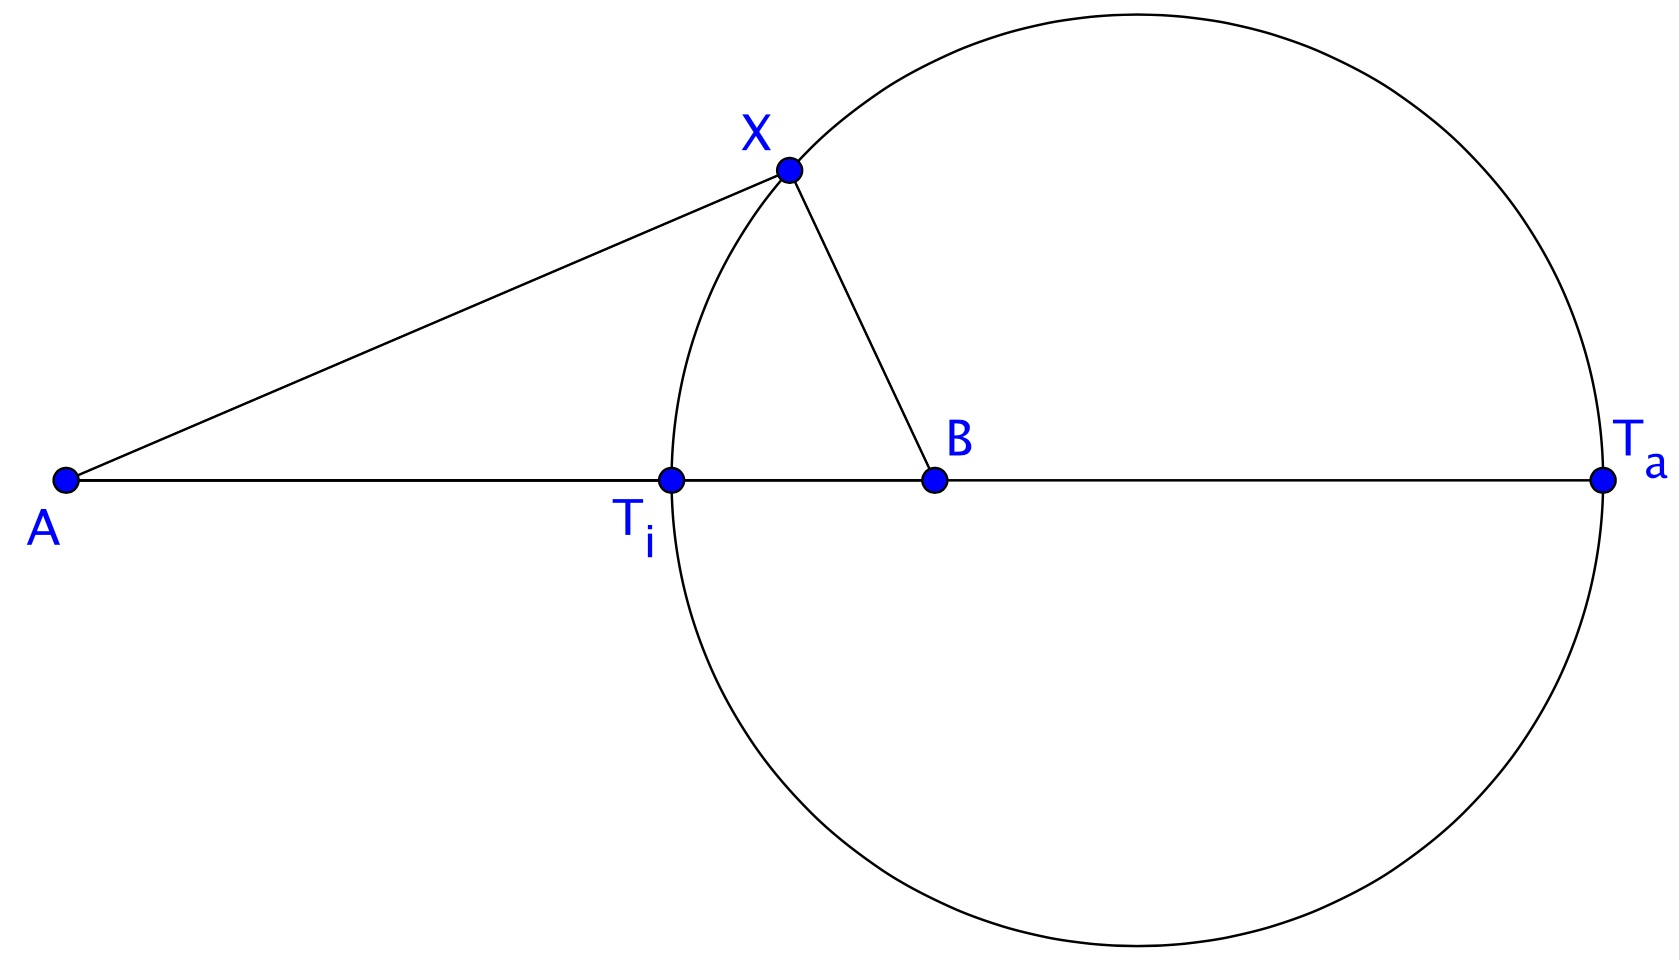
\includegraphics[width=3in]{Apollinus_anschaulich}
\\
Der Satz besagt also, dass alle Punkte $X$ deren Abst"ande zu $A$ ($\overline{AX}$) und zu $B$ ($\overline{XB}$) im Verh"altnis $\lambda$ stehen, auf einem Kreis liegen.\\
\end{Definition}
\newline

\begin{Beweis}
\\
\underline{Beweis:}
Anfangen kann man den den Beweis damit, dass man zwei Punkte sucht, die die Bedingung erf"ullen \textbf{und} auf der Geraden $AB$ liegen. Logisch ist, dass einer dieser Punkte zwischen $A$ und $B$ sein wird, dieser wird \textbf{innerer Teilungspunkt} $T_{i}$ genannt. Der andere Punkt liegt au"serhalb der Strecke $[AB]$ und wird \textbf{"au"serer Teilungspunkt} $T_{a}$ genannt. \\
Im letzten Schritt des Beweises wird man anhand des Skalarprodukts zeigen, dass f"ur alle Punkte $X$, die ebenfalls die Verh"altnisgleichung erf"ullen, die Vektoren $\vv{T_{i}X}$ und $\vv{T_{a}X}$ orthogonal zueinander sind. Somit liegen diese Punkte auf dem Thaleskreis (frz.: Theoreme du triangle rectangle) "uber $T_{i}$ und $T_{a}$, der dann \textbf{Apolliniuskreis} genannt wird.\\
\begin{enumerate}


\item {Um uns die Arbeit so einfach wie m"oglich zu machen, platzieren wir unseren ersten Punkt $A$ auf den Ursprung eines Koordinatensystems und die Strecke $[AB]$ entlang der $x$-Achse . Der Punkt $B$ hat den Abstand $\overline{AB}$ zu $A$, den man $b$ abk"urzt. Gleicherma"sen verf"ahrt man mit den L"angen $\overline{AT_{i}}=t_{i}$ und $\overline{AT_{a}}= t_{a}$, und man f"uhrt den Punkt $X(x|y)$ ein.\\
Hier nochmal ein "Uberblick:\\
\\
\vartriangleright $A(0|0)$ \qquad \vartriangleright $B(b|0)$ \qquad \vartriangleright $T_{i}(t_{i}|0)$ \qquad \vartriangleright $T_{a}(t_{a}|0)$ \qquad \vartriangleright $X(x|y)$\\
\\}

\item {Nun gilt:
\begin{center}
$\dfrac{\overline{AT_{i}}}{\overline{T_{i}B}} = \lambda$ \qquad und \qquad $\dfrac{\overline{AT_{a}}}{\overline{T_{a}B}} = \lambda$ \\
\end{center}
Das benutzt man, um die Koordinaten $t_{i}$ und $t_{a}$ in Abh"angigkeit von $b$ und $\lambda$ auszudr"ucken, denn diese Punkte sind ja durch das Verh"altnis $\lambda$ in der Ebene festgelegt.\\

\begin{minipage}[t]{0.5\textwidth}
\begin{array}{rccl}
&$\dfrac{\overline{AT_{i}}}{\overline{T_{i}B}}$ & $=$ & $\lambda$\\
$\Leftrightarrow & \dfrac{t_{i}}{b-t_{i}} $& $= $& $\lambda$\\
$\Leftrightarrow & $t_{i}$&$=$&$\lambda \cdot b - \lambda \cdot t_{i}$\\
$\Leftrightarrow & \lambda \cdot t_{i} + t_{i}$ &$=$& \lambda \cdot b$\\
$\Leftrightarrow & (\lambda + 1)\cdot t_{i}$&$=$& $\lambda \cdot b$\\
$\Leftrightarrow & t_{i} $&$=$& $ \dfrac {\lambda}{\lambda +1}\cdot b$
\end{array}
\end{minipage}
\begin{minipage}[t]{0.5\textwidth}
\begin{array}{rccl}
&$\dfrac{\overline{AT_{a}}}{\overline{T_{a}B}} $&$ = $&$ \lambda$\\
$\Leftrightarrow $&$ \dfrac{t_{a}}{t_{a}-b} $&$ = $& $\lambda$\\
$\Leftrightarrow & $t_{a}$&$=$&$\lambda \cdot t_{a} - \lambda \cdot b$\\
$\Leftrightarrow & \lambda \cdot t_{a} - t_{a} $&$=$&$\lambda \cdot b$\\
$\Leftrightarrow & (\lambda -1 \cdot )t_{a} $&$=$&$\lambda \cdot b$\\
$\Leftrightarrow & t_{a} $&$=$&$ \dfrac{\lambda}{\lambda -1}\cdot b$\\
\end{array}
\end{minipage}}
\\
\item{ Jetzt wo wir $T_{i}$ und $T_{a}$ in Abh"angigkeit von $b$ und $\lambda$ bestimmt haben, kann man die Vorraussetzung auch noch auf den Punkt $X$ anwenden.\\
\\
\begin{array}{rcccl}
&$\dfrac{\overline{AX}}{\overline{XB}}$ & $=$ & $\lambda$ \\
$\Leftrightarrow & $(\dfrac{\overline{AX}}{\overline{XB}})^2$ & $=$ & \lambda^2$\\
$\Leftrightarrow & $\dfrac{(\overline{AX})^2}{(\overline{XB})^2}$ & $=$ & \lambda^2$\\
$\Leftrightarrow & $\dfrac{x^2+y^2}{(x-b)^2+y^2} $ & $=$ & $\lambda^2$\\
$\Leftrightarrow & $x^2+y^2$ & $=$ & $\lambda^2 \cdtot [(x-b)^2+y^2]$\\
$\Leftrightarrow & $0$ & $=$ & $\lambda^2 \cdot (x-b)^2 +\lambda^2 y^2 -x^2 -y^2$\\
$\Leftrightarrow & $0$ & $=$ & $x^2\cdot \lambda^2 - 2bx\cdot \lambda^2 +b^2\cdot \lambda^2 +y^2\cdot \lambda^2 -x^2-y^2 $ &\textcolor{red}{(1)}\\
\\
\end{array}
}



\item{
Bevor man zum Ende kommt, kann man noch die Ergebnisse aus 2) benutzen, um $t_{i}$ und $t_{a}$ miteinander zu verrechnen, denn diesen Zusammenhang braucht man gleich.\\
\begin{center}
\begin{array} {rccccccl}
$t_{i} + t_{a} $ & $=$ & $\dfrac {\lambda}{\lambda +1}\cdot b + $\dfrac {\lambda}{\lambda -1}\cdot b  $ &$=$& $(\dfrac{\lambda}{\lambda+1} + \dfrac{\lambda}{\lambda-1})\cdot b$ & $=$ & $\dfrac{\lambda^2}{\lambda^2 -1}\cdot 2b$ \qquad \textcolor{red}{(2)}\\
\end{array}
\\
\begin{array} {rcccccl}
$t_{i} \cdot t_{a} $ & $=$ & $\dfrac {\lambda}{\lambda +1}\cdot b \cdot $\dfrac {\lambda}{\lambda +1}\cdot b $ & $=$ & $\dfrac{\lambda^2}{\lambda^2 -1}\cdot b^2$ \qquad \textcolor{red}{(3)}\\ \\
\end{array}
\end{center}
}

\item{
Nun kommt der finale Schritt. Man bildet die Vektoren $\vv{T_{i}X} = \left(\begin{array}{c} x-t_{i} \\ y \end{array}\right)$ und $\vv{T_{a}X} = \left(\begin{array}{c} x-t_{a} \\ y \end{array}\right)$ und berechnet deren Skalarprodukt. $\ast$ TROMMELWIRBEL$\ast$ \\
\\
\begin{center}
\begin{array}{rccl}
$\vv{T_{i}X} \cdot \vv{T_{a}X}$ &$=$& $(x-t_{i})\cdot (x-t_{a}) +y^2$\\
& $=$ & $x^2 -(t_{i} +t_{a})x + t_{i}\cdot t_{a} + y^2$ & $Benutze (2) und (3) \\
& $=$ & $x^2 - \dfrac{\lambda^2}{\lambda^2 - 1} \cdot 2bx + \dfrac{\lambda^2}{\lambda^2 - 1} \cdot b^2 +y^2$\\
& $=$ & $\dfrac{x^2 \cdot (\lambda^2 -1) - 2bx\cdot \lambda^2 + b^2\cdot \lambda^2 + y^2 \cdot (\lambda^2 -1)}{\lambda^2 -1}$\\
& $=$ & $\dfrac{x^2 \cdot \lambda^2 - 2bx\cdot \lambda^2 b^2\cdot \lambda^2 +y^2\cdot \lambda^2 -x^2 -y^2} {\lambda^2 -1}$ &  $Benutze (1) \\
& $=$ & $0$\\
\\
\end{array}
\end{center}
}

Damit hat man bewiesen, dass f"ur alle Punkte $X$ die Vektoren $\vv{T_{i}X}$ und $\vv{T_{a}X}$ orthogonal zueinander sind, weshalb sie auf dem Thaleskreis "uber $T_{i}$ und $T_{a}$ liegen m"ussen.\\ \\
\end{enumerate}
\end{Beweis}


Die Figur und die Zusammenh"ange, die man durch den Satz des Apollinius erhalten hat, kann man benutzen, um ein wenig mit Winkeln zu spielen: \\
\\
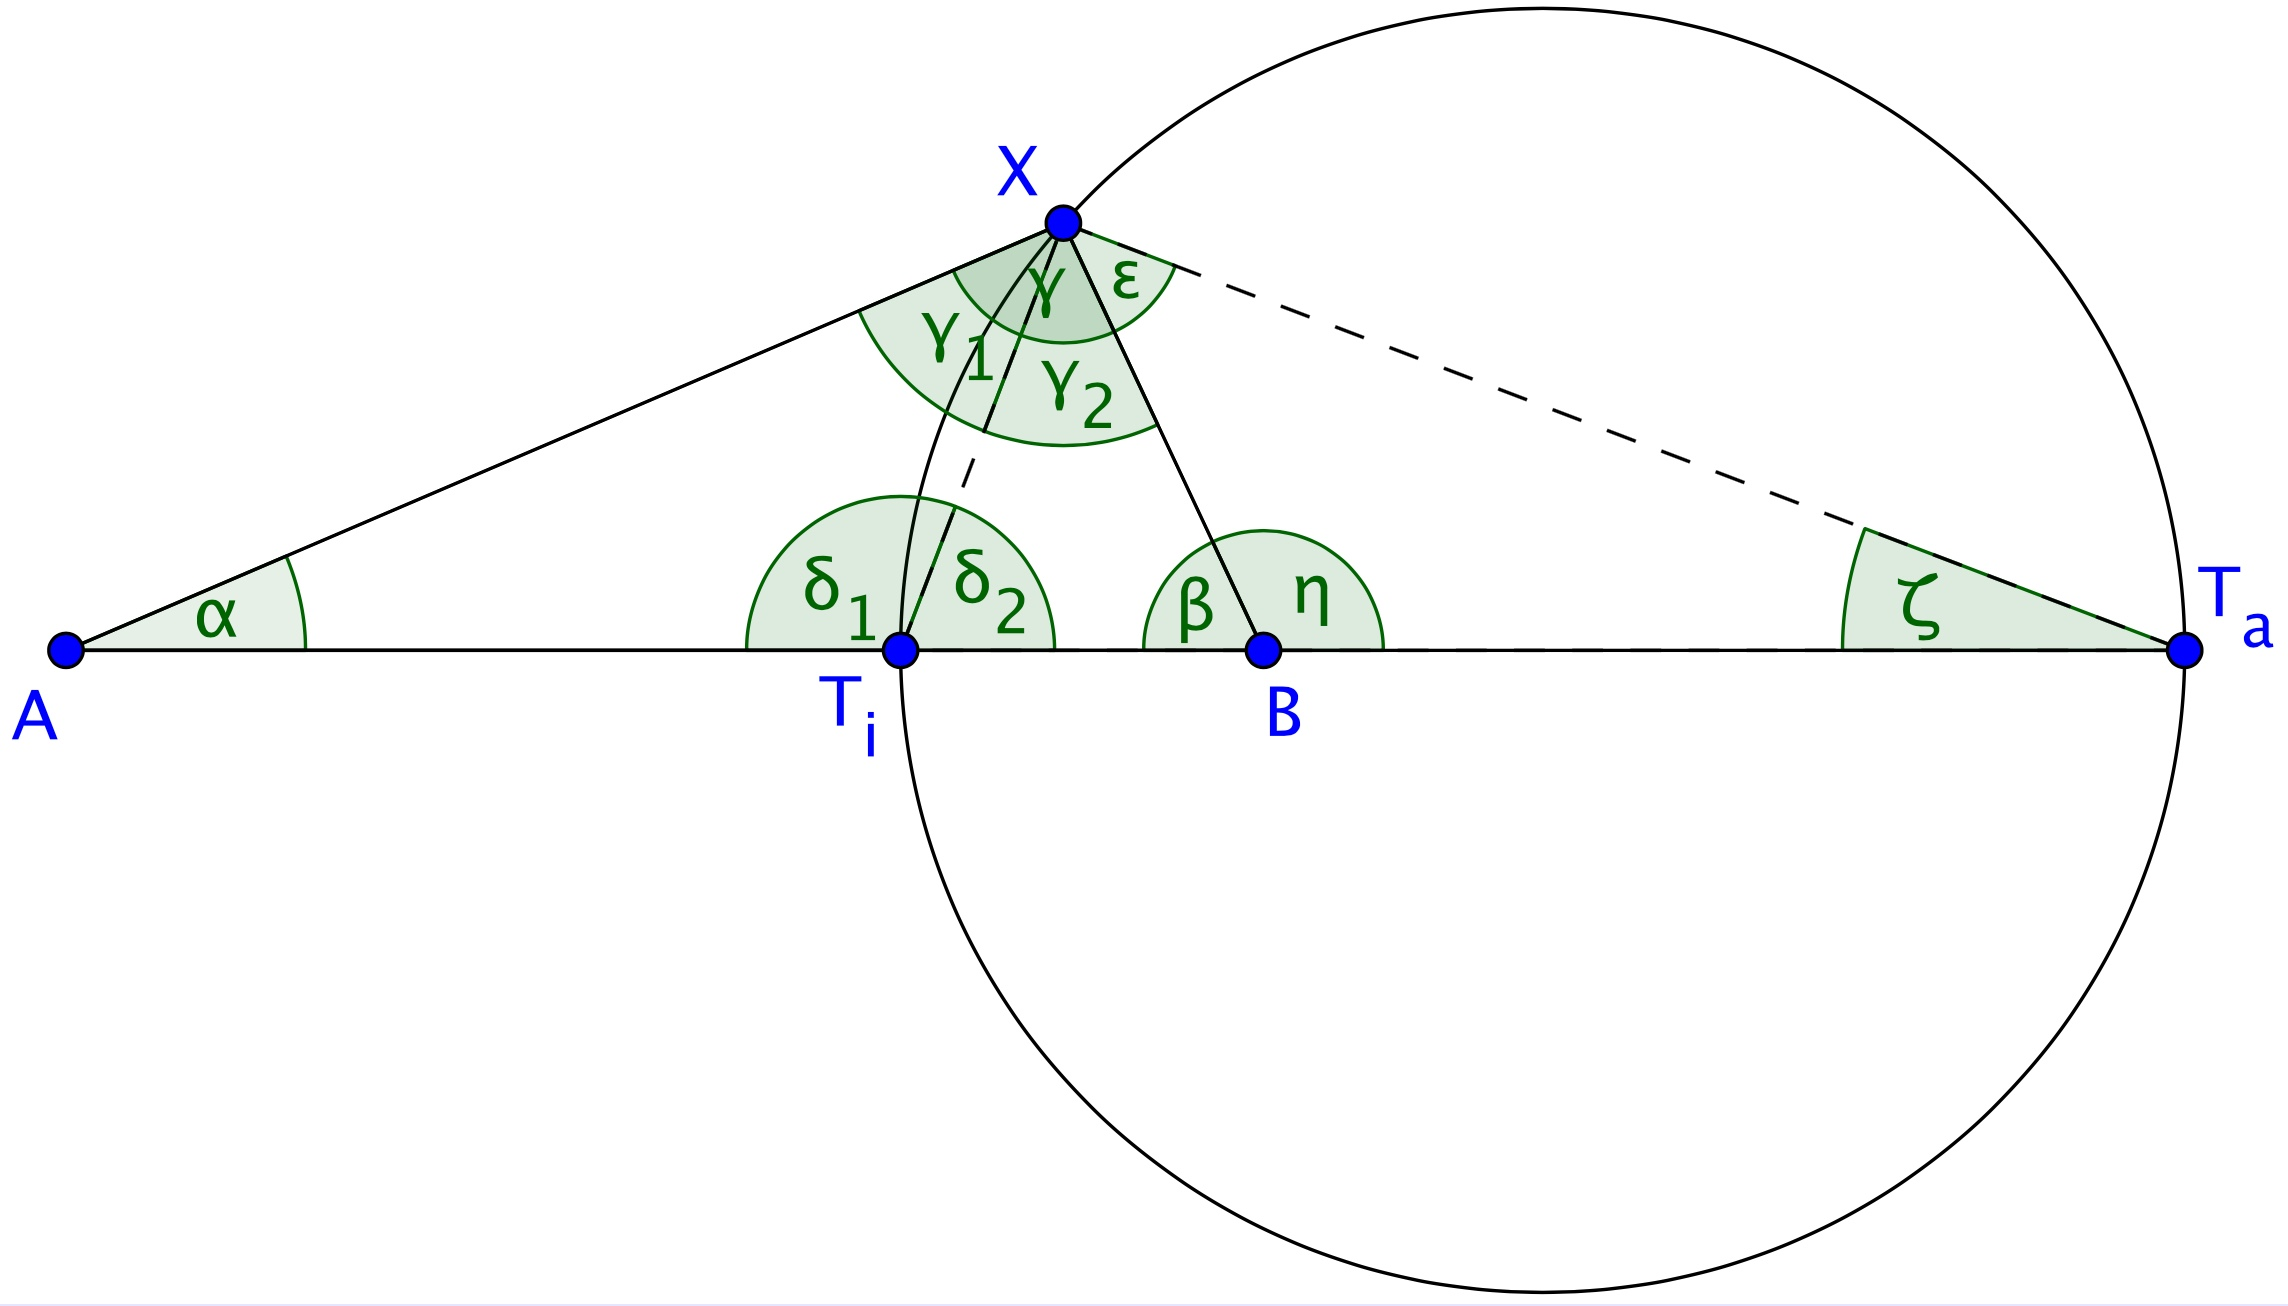
\includegraphics[width=5in]{Apollinius_Winkel}\\
\\
\begin{mdframed}
Auf dieser Skizze sind 10 Winkel gekennzeichnet, zu welchen sich eine ganze Reihe von Beziehungen aufstellen l"asst:\\
\\
\begin{array}{rcccl}
$\vartriangleright \alpha + \beta + \gamma = 180 $ & $\vartriangleright \beta + \gamma_{2} + \delta_{2} = \ang{180} $ & $\vartriangleright \delta_{1} + \delta_{2} = \ang{180} $ & $\vartriangleright \alpha + \gamma + \epsilon + \zeta = \ang{180} $ &$\vartriangleright \epsilon + \zeta + \eta = \ang{180}$\\
$\vartriangleright \aplha + \gamma_{1} + \delta_{1} = \ang{180} $ & $\vartriangleright \gamma_{1} + \gamma_{2} = \gamma $ & $\vartriangleright \gamma_{2} + \epsilon = \ang{90} $ & $\vartriangleright \beta + \eta = \ang{180} $ &$\vartriangleright \gamma_{2} + \delta_{2} + \epsilon + \zeta = \ang{180}$\\
\\
\end{array}
\\
Hiermit bekommt man ein zehndimensionales Gleichungssystem mit dem sich $\gamma_{1} = \gamma_{2}$ zeigen l"asst. Dies bedeutet dass die Gerade $T_{i}X$ auch noch die Winkelhalbierende des Winkels $\gamma = \angle AXB$ ist:
\\
\end{mdframed}
\begin{Definition}
Eine Innenwinkelhalbierende eines Dreiecks teilt die gegen"uberliegende Seite im Verh"altnis der Anliegenden Seiten. \qquad $\gamma_{1}=\gamma_{2} \Rightarrow \overline{AT_{i}}:\overline{T_{i}B}=\overline{AX}:\overline{XB}$
\end{Definition}
 \begin{center}
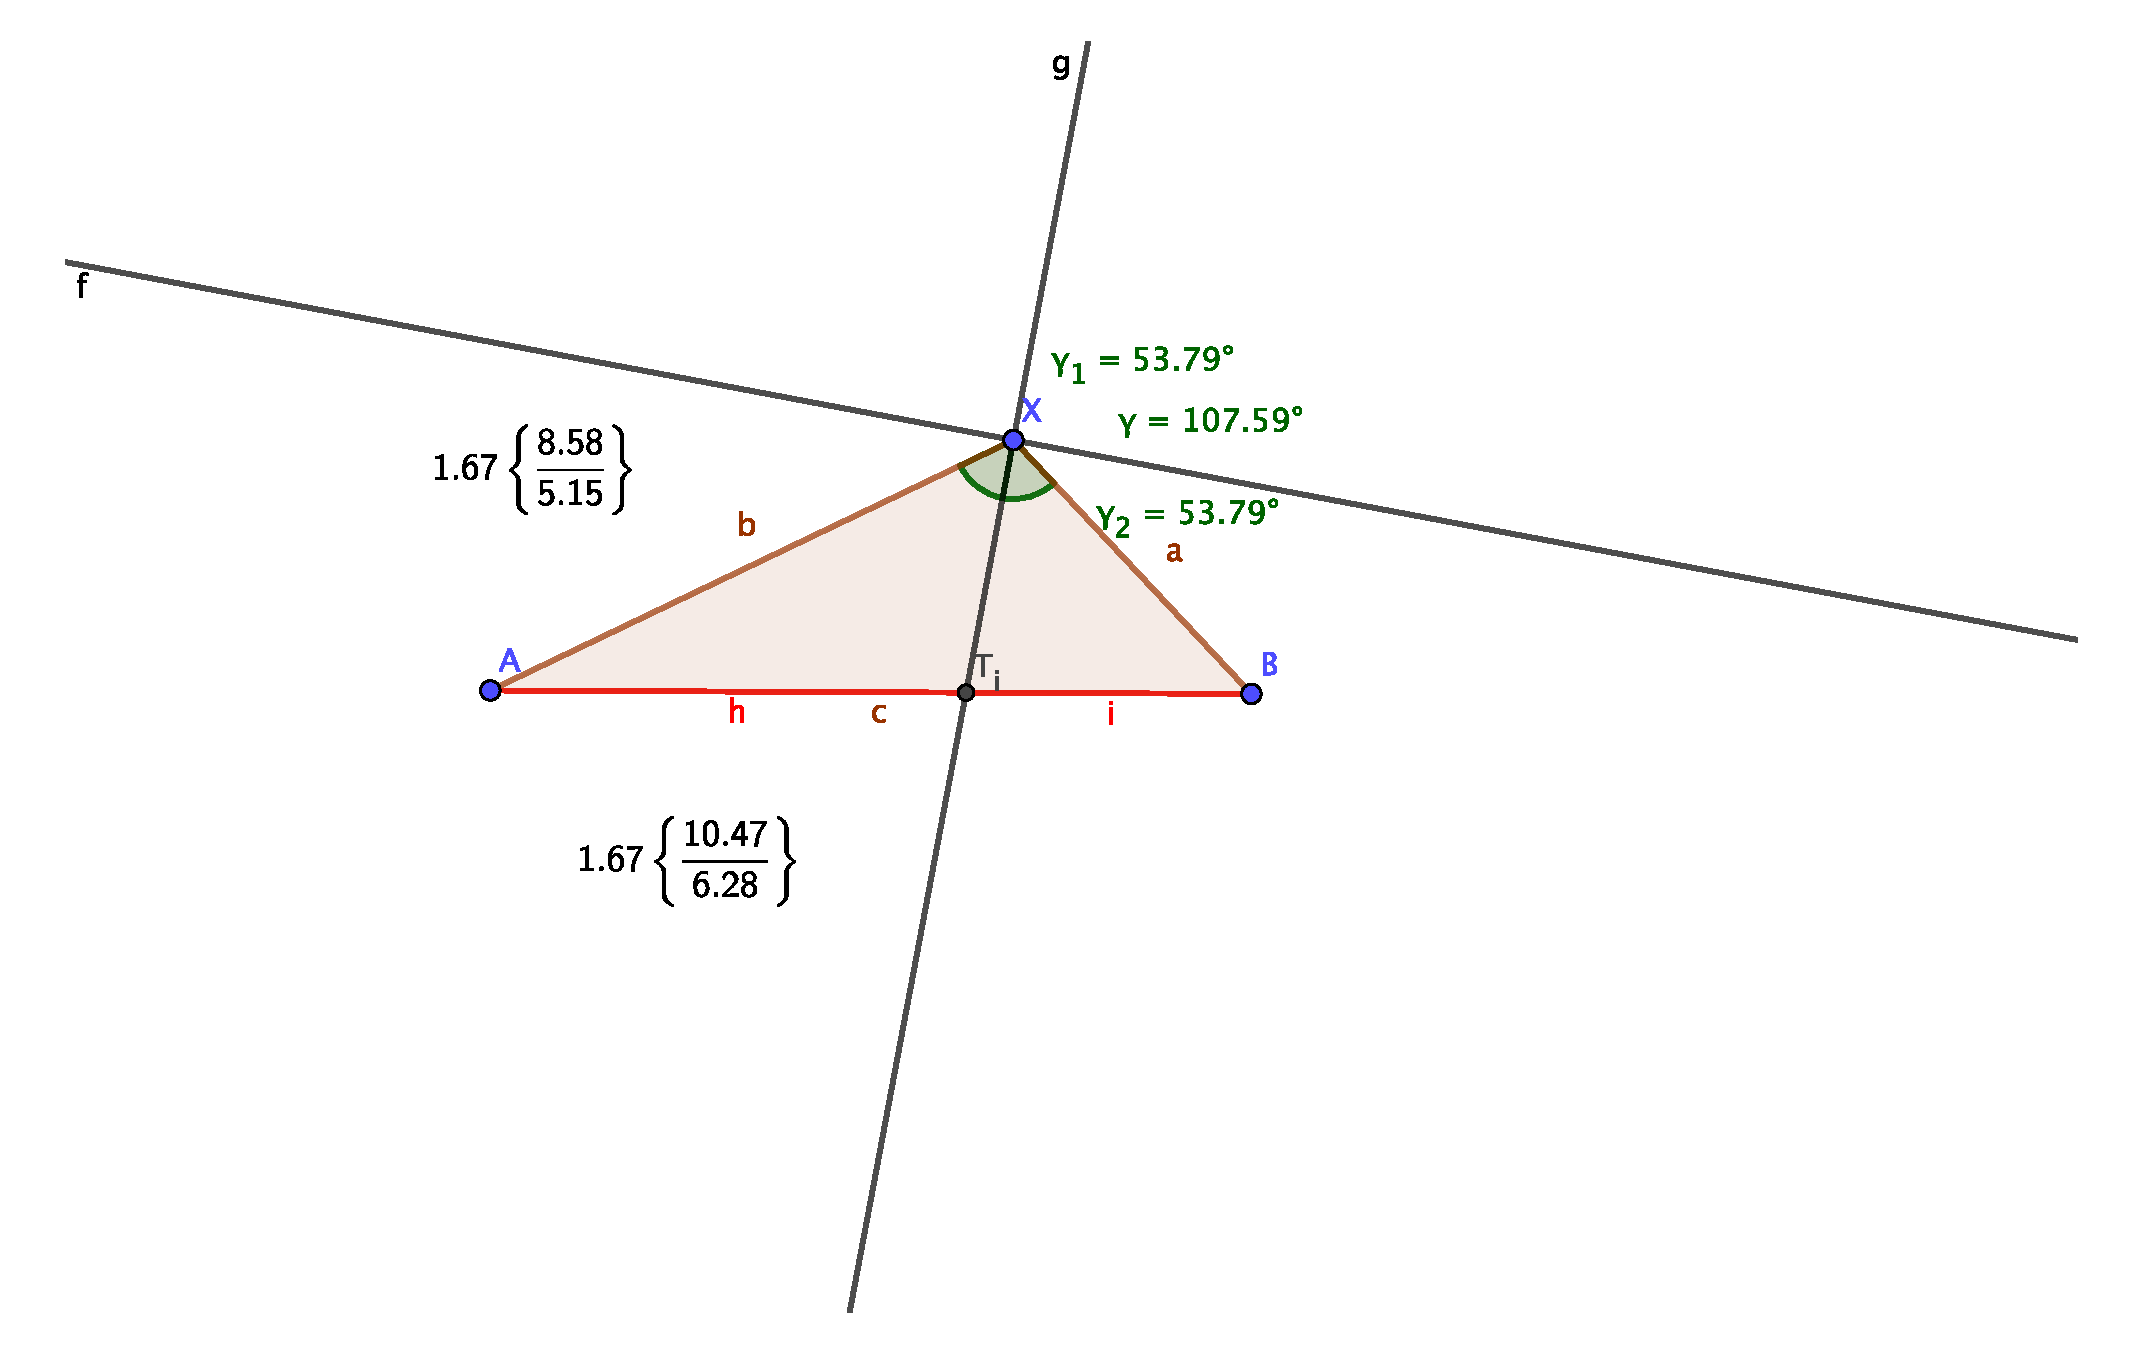
\includegraphics[width=4.7in]{Apollinus_Winkelhalbierende_Bild}
\end{center}
\end{small}
Quelle (Apollinus) : Tobias Rave, 06.03.18, Skript 1ere SBC S.68-71

  \chapter{Komplexe Zahlen}


\section{Einführung}

	\paragraph{} Die Ursache für die Einführung der komplexen Zahlen ist vergleichbar mit der jeglicher anderer Zahlenmengen (abgesehen
	von $\N$). Alles basiert auf einer Rechnung oder einer Menge an Rechnungen, welche für die vorhandenen Zahlenmengen \textbf{keine Lösung besitzen} oder aber diese Zahlenmengen einem nicht erlauben eine Lösung zu finden. Ein Beispiel hierfür ist die Einführung der
	negativen Zahlen. Gleichungen der Form $2 + x = 1$ waren eine Zeit lang nicht lösbar. Ebenso galt einmal, dass $x^2 - 2 = 0$ keine
	Lösung besitzt, da hierfür die reellen Zahlen benötigt werden. Analog dazu wird die Erweiterung auf die komplexen Zahlen begründet.
	Dies wird an folgendem klassischen Beispiel erläutert:

	\begin{align*}
		\qquad \qquad x^2 + 1 &= 0 \\
			\Leftrightarrow x &= \sqrt{-1} \quad \text{\Lightning}
	\end{align*}

	\paragraph{} Um dieser und anderen Gleichungen eine Lösung zuzuteilen ist es nicht nur notwendig die Zahlenmenge zu erweitern, sondern
	auch, neue Symbole und Zeichen einzuführen um die neuen Zahlen zu kennzeichnen. Für die $\Z$ ist es das Symbol \dq-\dq, für $\Q$
	\dq,\dq und $\dfrac{a}{b}$, für $\R$ $\sqrt{a}$ und die Zeichen $\pi$ und $e$ zum Beispiel (auch wenn beide sich anders darstellen lassen). (Ein) gewisse(r) Mathematiker (Leibniz glaube ich) hat entschieden, dass das einzige benötigte Zeichen $i$ sein sollte, da er sie imaginäre Zahl nannte (Für den Fall, dass ich hier ein bisschen was durcheinander bringe, sind Direktverbesserungen kommentarlos erlaubt und erwünscht).
 	Und dem war so, weshalb nun gilt:
											$$i \in \C : i^2 = -1; \C \definedBy \R \cup \left\{i\right\}$$

	\begin{Definition}
		Komplexe Zahlen werden standartmäßig mit dem Buchstaben $z$ dargestellt. Die allgemeine Formel einer solchen Zahl lautet:
		\\
		\begin{tikzpicture}
			\draw (0,0) node {" "};
			\draw (7.9, 0) node {$z = x + y \cdot i; x,y \in \R; i \in \C$};
			\draw[line width=0.8pt][decorate,decoration={brace,amplitude=3pt},rotate around={180:(7.6,-0.25)}] (7.6,-0.25) -- (8.1,-0.25);
			\draw[line width=0.8pt][decorate,decoration={brace,amplitude=2pt},rotate around={180:(6.7,-0.25)}] (6.7,-0.25) -- (7,-0.25);
		    \draw[line width=0.4pt] (6.55,-0.5) -- (5.1,-1.4) node[color=blue,left] {$Re(z)$};
		    \draw[line width=0.4pt] (7.35,-0.5) -- (9.2,-1.4) node[color=blue,right] {$Im(z)$};
		\end{tikzpicture}
		\\
		Hierbei wird $x = Re(z)$ Realteil und $y = Im(z)$ und zwar \textbf{nur $y$} Imaginärteil genannt.
	\end{Definition}

	\begin{Bemerkung}
		Eine Zahl $z = x + yi \in \C$ heißt rein imaginäre Zahl für $x = 0$. Analog dazu wird sie für $y = 0$ als reell bezeichnet.
	\end{Bemerkung}


\section{Der Körper der komplexen Zahlen}

	\paragraph{} Da wir nun wissen (oder halt auch nicht), weshalb wir die komplexen Zahlen benötigen, gilt es nun die verschiedenen Verknüpfungen, mit welchen wir zwei komplexe Zahlen verbinden, zu definieren. Wie alle anderen bekannten Mengen (außer $\N$), ist $\C$ teil eines \textbf{Körpers} welcher die zwei Verknüpfungen, denen wir allgemein die Namen \textbf{Addition} und \textbf{Multiplikation} geben. Das 3-Tupel (oder auch Tripel) ($\C$, +, *) ist somit der Körper, mit welchem wir arbeiten werden (jemals gefragt warum keine weiteren Verknüpfungen eingeführt wurden?). Jedoch muss auch erstmal bewiesen werden, dass dieses Tripel ein Körper ist:

	\begin{Beweis}
		\underline{\textbf{Die Addition}}:

		\paragraph{} Für die Addition gilt bekanntlich zu beweisen, dass ($\C$, $\oplus$) eine abelsche oder auch kommutative Gruppe ist:

		\begin{enumerate}[1)]
			\item \begin{align*}
						\forall z_1, z_2 \in \C: z_1 \oplus z_2 &\definedBy (x_1 + y_1i) \oplus (x_2 + y_2i) \\
														   		&= ((x_1 + x_2) + (y_1 + y_2)i) \\
														   		&\in \C \\
						\Rightarrow \forall z_1, z_2 \in \C: \oplus : \C \times \C \rightarrow \C & \quad \text{(Abgeschlossenheit)}
				  \end{align*}
			\item \begin{align*}
				  		(z_1 \oplus z_2) \oplus z_3 &= ((x_1 + x_2) + (y_1 + y_2)i) \oplus (x_3 + y_3i) \\
										  			&= ((x_1 + x_2 + x_3) + (y_1 + y_2 + y_3)i) \\
												    &= (x_1 + y_1i) \oplus ((x_2 + x_3) + (y_2 + y_3)i) \\
												    &= (x_1 + y_1i) \oplus ((x_2 + y_2i) \oplus (x_3 + y_3i)) \\
												    &= z_1 \oplus (z_2 \oplus z_3) \\
						\Rightarrow \forall z_1, z_2, z_3 \in \C: (z_1 + &z_2) \oplus  z_3 = z_1 \oplus (z_2 + z_3) \quad \text{(Assoziativität)}
				  \end{align*}
			\item \begin{align*}
						e = (0 + 0i) \in \C, \forall z \in \C:& \\
												   z \oplus e = (x + yi&) \oplus (0 + 0i) \\
													  		  = ((x + 0&) + (y + 0)i) \\
															  = (x + yi&) \\
						\Rightarrow \exists e: z \oplus e = z; z \in \C \quad &\text{(Neutrales Element)}
				  \end{align*}
			\item \begin{align*}
	  					z* = -(x + yi) \in \C, z \in \C \text{ (Hierbei gilt es z* nicht} & \text{mit $\overline{z}$ zu verwechseln)}: \\
								  z \oplus z* = (x + yi) \oplus (-(x + yi)) \text{          } & \\
								  			  = ((x - x) + (y - y)i) \text{ 				} & \\
											  = (0 + 0i) \text{ 							} & \\
											  = e \text{								    } & \\
						\Rightarrow \exists z*: z \oplus z* = e; z \in \C \quad \text{(Inverses Element)} \qquad &
	  			  \end{align*}
			\item \begin{align*}
						z_1 \oplus z_2 &= (x_1 + y_1i) \oplus (x_2 + y_2i) \\
									   &= ((x_1 + x_2) + (y_1 + y_2)i) \\
									   &= ((x_2 + x_1) + (y_2 + y_1)i) \\
									   &= (x_2 + y_2i) \oplus (x_1 + y_1i) \\
									   &= z_2 \oplus z_1 \\
						\Rightarrow \forall z_1, z_2 \in \C: z_1 \oplus z_2 = z_2 \oplus z_1 \quad \text{(Kom}&\text{mutativität)}
				  \end{align*}
		\end{enumerate}
		\\
		\\
		\underline{\textbf{Die Multiplikation}}:
	\end{Beweis}

\section{Die Gauß'sche Zahlenebene}

	\paragraph{} Da jetzt der Körper der komplexe Zahlen definiert wurde, gilt es ihn nun in unser bekanntes Zahlensystem zu integrieren.
	Hierfür kann man zum Beispiel beobachten, wie sich komplexe Zahlen auf der \textbf{reellen Zahlengerade} (welche eine Veranschaulichung des euklidischen Vektorraums $\R^1$ ist) verhalten:
	\\
	\begin{center}
		\begin{tikzpicture}[>=triangle 45]
			\draw[line width=0.8pt] (0,0) -- (-5,0);
			\draw[line width=0.8pt] (0,0) -- (5,0);
			\foreach \x in {-5,-4,...,-1,1,2,...5}
				\draw[line width=0.8pt] (\x,0.5) -- (\x,-0.5) node[below] {\x};
			\draw[line width=0.8pt,color=blue] (-0.25,-0.25) node {$O$};
		\end{tikzpicture}
	\end{center}
	\\
	\paragraph{} Zunächst muss verstanden werden, welche Transformation jeweils Addition und Multiplikation im $\R^1$ auf reelle Zahlen ausführt:
	\\
	\begin{center}
		\begin{tikzpicture}[>=triangle 45]
			\draw[line width=0.8pt] (0,0) -- (-5,0);
			\draw[line width=0.8pt] (0,0) -- (5,0);
			\foreach \x in {-5,-4,...,-1,1,2,...5}
				\draw[line width=0.8pt] (\x,0.5) -- (\x,-0.5) node[below] {\x};
			\draw[line width=0.8pt, color=blue] (-0.25,-0.25) node {$O$};
			\draw[line width=0.8pt, color=blue] (3,0.6) node {3};
			\draw[line width=0.8pt, color=blue] (-3,0.6) node {-3};
		\end{tikzpicture}
	\end{center}

  \chapter{Algebra oder Zahlentheorie}
\chapterauthor{Bruno}

	\section{Körper}

Ein Körper ist eine Menge $K$, versehen mit zwei inneren zweistelligen Verknüpfungen $+$ und $\cdot$, also Addition und Multiplikation, für welche eine Addition
$$\oplus\quad : \quad K \times K \rightarrow K$$
$(a;b) \longmapsto a+b $\\\\
und eine Multiplikation
$$\odot \quad : \quad K \times K \rightarrow K$$
$(a;b) \longmapsto a \cdot b $\\\\\\
gegeben sind, sodass\\

\begin{array}{rcl}
\textcolor{titlepagecolor}{Assoziativgesetz} & $ (A1) & a+(b+c) = (a+b)+c $\\\\
\textcolor{titlepagecolor}{Kommutativgesetz} & $ (A2) & a+b = b+a$\\\\
\textcolor{titlepagecolor}{Neutrale\,\, Element} & $ (A3) & \exists ! \quad 0 \quad $ mit:  \\\\
&$ & a+0 = 0+a = a$\\\\
\textcolor{titlepagecolor}{Inverse\,\, Element} & $ (A4) & \forall a\in K \quad \exists ! -a \in K$  mit:  \\\\
$ & &a+(-a) = 0$\\\\\\
\textcolor{titlepagecolor}{Assoziativgesetz} & $ (M1) & a\cdot (b \cdot c) = (a\cdot b) \cdot c $\\\\
\textcolor{titlepagecolor}{Kommutativgesetz} & $ (M2) & a\cdot b = b\cdot a    $\\\\
\textcolor{titlepagecolor}{Neutrale\,\, Element} & $ (M3) & \exists ! \quad 1 \in K $ mit \\\\
&$ & 1\cdot a = a \cdot 1 = a $ \\\\
\textcolor{titlepagecolor}{Inverse\,\, Element} &$ (M4) & \exists ! \quad \dfrac{1}{a}$ \quad zu jedem $a \in K \backslash \{0\} $ mit: \\\\
$ && a \cdot \dfrac{1}{a} = 1 $\\\\\\
\textcolor{titlepagecolor}{Distributivgesetz} & $(D)$ & $a\cdot (b+c) = ab + ac$ \\
\end{array}\\\\\\

Dies erfüllen $\Q$, $\R$, $\R^{n}$ (Vektorräume), $\C$, Matritzen, prime Restklassengruppen $\Z / p\Z$ ...


	\section{Teilbarkeit}

	\subsection{Teilbarkeitseigenschaften}

\begin{Definition}
Die ganze Zahl $a\in\Z$ teilt $b\in\Z$, wenn es ein $x$ gibt, mit $b=a\cdot x$. Man schreibt:
$$a|b$$

$a$ ist ein \textbf{Teiler} von $b$ und $b$ ist \textbf{Vielfaches} von $a$\\\\

Zwei Zahlen $a,b\in\Z$  sind \textbf{teilerfremd}, wenn aus $ c | a  $ und $c|b$ folgt $|c|=1$
\end{Definition}

\begin{Theorem}
Aus dieser Teilbarkeitsrelation ergeben sich mehrere Eigenschaften:\\
Sei $a,b,c,t\in\Z$ und $t\neq0$:\\\\
(0)\qquad$a|b$ \quad und \quad&a|c& \quad dann \quad $a|b\pm c $\\
(1)\qquad$a|b$ \quad und \quad$b|c$ \quad dann \quad $a|c$\\
(2)\qquad$a|b$ \quad dann \quad $a|bc$\\
(3)\qquad$at|bt\quad\Leftrightarrow\quad a|b$\\
(4)\qquad$a|b$\quad dann \quad $b=0$ \quad oder\quad $|a| \leq |b| $\\
(5)\qquad$a|b$\quad und\quad $b|a$ \quad dann\quad $a=\pm b$
\end{Theorem}

\begin{Beweis}
\begin{itemize}
\item (1) \quad Wenn $a|b$ und $b|c$, dann gibt es $x,y\in\Z$ mit $b=a\cdot x$ und $c=b\cdot y$. Also gilt auch $c=b\cdot y=a\cdot(xy)$ und somit $a|c$\\
\item (2) \quad Weil offensichtlich $b|bc$ gilt, folgt die Aussage sofort aus Aussage (3) \\
\item (3)  \quad $at|bt\quad \Leftrightarrow\quad \exists x \in \Z : \, \, bt=atx \quad\Leftrightarrow \quad b=ax \quad\Leftrightarrow \quad a|b$ \\
\item (4) \quad Sei $b=ax$ mit $x\in\Z$. Wenn $x=0$, dann ist $b=0$. In alles anderen Fällen ist $|x|>1$ und daher $|b| = |a| \cdot |x| \geq |a|$
\item (5) \quad Wenn weder $a=0$ noch $b=0$ ist, dann folgt aus (4) $|a|\geq|b|\geq|a|$ und daher $a=\pm b$. Wenn also  $a=0$, dann folgt $b=0$
\end{itemize}
\end{Beweis}

	\subsection{Euklidische Division}

\begin{Definition}
Seien $a$ und $b$ zwei natürliche Zahlen. Es gibt dann immer $q,r \in \N$ sodass
$$a= b\cdot q + r \qquad 0\leq r < b$$
$q$ heißt \textbf{Quotient} und $r$  heißt \textbf{Rest}.
Man schreibt: \qquad $q=a \div b$ \qquad und \qquad $r \equiv a \mod b$
\end{Definition}

	\section{Primzahlen}

Hier die Liste der Primzahlen bis 100: \\

2,     3,     5,     7,    11,    13,    17,    19,    23,    29,    31,    37,    41,    43,    47,    53,    59,    61,    67,    71,    73,    79,    83,    89,    97\\\\

\begin{Definition}
Eine natürliche Zahl heißt Primzahl, wenn sie in $\N$ genau zwei Teiler besitzt.
\end{Definition}


\begin{Theorem}
Es gibt unendlich viele Primzahlen
\end{Theorem}


\begin{Beweis}
Es gibt unendlich viele Primzahlen: Beweis nach Euklid\\\\

Jede ganze Zahl $n>1$ ist durch eine Primzahl teilbar. Entweder ist $n$ selber eine Primzahl oder $n=a\cdot b$ mit $a,b\in\N$.\\
Also ist $1<a=\dfrac{n}{b}<n$. Wenn man diesen Schritt endlich oft macht, kommt man am Ende auf ein neues $a'\in\mathbb{P}$.\\
$\A$: Nehmen wir jetzt an, es gäbe nur endlich viele Primzahlen $p_{1},p_{2},...,p_{r-1},p_{r}$.\\\\
Dann ist $$N=p_{1}\cdot p_{2}\cdot ... \cdot p_{r-1} \cdot p_{r} +1 = \left(\prod_{r=1}^{r}P_{r}\right) + 1 $$ eine ganze Zahl $>1$ und hat daher mindestens einen Primteiler $p_{l} \in\mathbb{P}$ und $l\in\{1,2,...,r-1,r\}$
Dann hat man:\\

$\Rightarrow$ $\left\{ \begin{array}{rccl}
$p_{l} & | & p_{1}\cdot p_{2}\cdot...\cdot p_{r-1}\cdot p_{r}$\\
$p_{l} & | & p_{1}\cdot p_{2}\cdot...\cdot p_{r-1}\cdot p_{r} +1$\\
\end{array}\right.\\


$\Leftrightarrow p_{l} | \, p_{1}\cdot p_{2} \cdot...\cdot p_{r-1} \cdot p_{r} - \left(  p_{1}\cdot p_{2} \cdot...\cdot p_{r-1} \cdot p_{r} +1 \right)$\\\\
$\Leftrightarrow p_{l} | \, (-1) \quad $oder$ \quad p_{l} | 1$ \qquad   WIDERSPRUCH, da $p_{l}=1$ aber $1\notin \mathbb{P}$ \\\\
$N$ muss also einen Primteiler haben ungleich $p_{r} \quad mit \quad r\in\{1,2,3,...,r-1,r\}$ oder \textbf{selber prim sein}.
\end{Beweis}


\begin{Theorem}

Jede natürliche Zahl $n\geq2$, die nicht prim ist, besitzt einen Primfaktor $p$, für den gilt
$$p^2\leq n \quad\Leftrightarrow\quad p\leq \sqrt{n}$$
Also lässt sich jede Zahl, die nicht prim ist, in Primfaktoren zerlegen.\\

Jede natürliche Zahl $n\geq2$ besitzt eine eindeutige \textbf{Primfaktorzerlegung} der Form
$$n=(p_{1})^{a_{1}} \cdot (p_{2})^{a_{2}} \cdot ... \cdot (p_{k-1})^{a_{k-1}} \cdot (p_{k})^{a_{k}}   $$
mit $p_{1}< p_{2}< ... < p_{k-1}< p_{k}$ \quad und \quad $ \left\{ p_{1}, p_{2}, ... , p_{k-1}, p_{k} \right\} \in \mathbb{P}$ \quad und \quad $a_{1}, a_{2}, ...  a_{k-1}, a_{k} \in \N $


\end{Theorem}


	\section{Restklassen oder Kongruenzklassen}

\begin{Definition}
Seien drei natürliche Zahlen $a, b, n \in \N$ mit $n\geq 2$.\\ Wenn $a=q_{1} \cdot n + r_{1}$  \qquad und \qquad  $b=q_{2} \cdot n + r_{2}$ \qquad und \quad $r_{1}=r_{2}$,\qquad also falls $a$ und $b$ bei der euklidischen Division durch $n$ den gleichen Rest besitzen, dann gilt
$$a \equiv b\mod n$$
\end{Definition}

\begin{Beispiel}
\begin{itemize}
\item $29\equiv-121 \mod 5 $ \quad da $29 \equiv 5\cdot 5 +4$ \quad und \quad $-121 = 5\cdot (-25) +4$
\item $88\equiv 24 \mod 8 $ \quad da $8|88$ \quad und \quad $8|24$
\item $87\equiv 23 \mod 8$ \\
\end{itemize}
\end{Beispiel}

\begin{Theorem}
Seien $a,b$ zwei ganze Zahlen und $n\in\N$ mit $n\geq 2$, dann gilt\\\\
(1)\qquad $ a\equiv b \mod n \quad \Leftrightarrow \quad n|(a-b)$\\
(2)\qquad $ a\equiv 0 \mod n \quad\Leftrightarrow\quad n|a$\\
(3)\qquad falls $n'\geq 2$ und $n'|n$ dann gilt: \quad $a \equiv b \mod n \quad \Rightarrow \quad a \equiv b \mod n' $\\\\
\end{Theorem}

\begin{Beweis}
\begin{itemize}
\item (1) \quad $ a \equiv b \mod n \quad\Leftrightarrow\quad a - b \equiv 0 \mod n \quad\Leftrightarrow\quad $ $n$ teilt $(a-b)$
\end{itemize}
\end{Beweis}

\begin{Beispiel}
\begin{itemize}
\item (1) \quad $61 \equiv 29 \mod 8$ \quad (Rest 5) $\quad\Leftrightarrow\quad 8| (61-29) = 32 $
\item (3) \quad $4 \geq 2$ \, und \, $4|12$ \quad $43 \equiv 67 \mod 12 \quad(r=7)\qquad \Rightarrow \quad 43 \equiv 67 \mod 4  $ \\
\end{itemize}
\end{Beispiel}

\begin{Theorem}
Für jedes $n\in \N$ mit $n\geq 2$ gilt: \\Jede ganze Zahl $a$ ist modulo $n$ kongruent zu einer natürlichen Zahl $r$ mit $0 \geq r \geq n-1$\\\\
Anders gesagt gibt es zu jeder Zahl immer Kongruenzklassen.
\end{Theorem}

\vspace{2em}

\begin{Definition}
Es seien $n \in \N$ mit $n \geq 2$ und $r \in \N$ mit $0 \leq r < n$ \\
Die Menge $ [r] \mod n $ ist die Menge aller ganzen Zahlen $z$, die bei der euklidischen Division durch $n$ den Rest $r$ liefern.\\\\
Sie ist eine Menge von Zahlen, die den Abstand $n$ zueinander haben.\\\\\\
Kongruenzen sind mit der Addition und der Multiplikation verträglich. Seien $a, b, a^{*}, b^{*}$ ganze Zahlen:\\\\
 $\Rightarrow$ $\left\{ \begin{array}{rcl}
$ a & \equiv & a^{*} \mod n  $\\
$ b & \equiv & b^{*}\mod n  $
\end{array}\right.\\\\
$\Rightarrow a+b \equiv a^{*} + b^{*} \mod n$ \qquad und \qquad  $a\cdot b \equiv a^{*} \cdot b^{*} \mod n$\\
\end{Definition}

\begin{Beispiel}
\begin{itemize}
\item $ [1] \mod 4 = \{ ... , -7, -3, 1, 5, 9, ... \} $
\item $ [2] \mod 4 = \{ ... , -6, -2, 2, 6, 10, ... \} $
\item $ [3] \mod 4 = \{ ... , -5, -1, 3, 7, 11, ... \} $
\item $ [4] \mod 4 = [0] \mod 4 = \{ ... , -8, -4, 0, 4, 8, 12, ... \} $\\
\end{itemize}
\end{Beispiel}

\begin{Theorem}
Seien $a,b \in \N$ mit \quad $a,b \geq 2$ \quad und $a|b$, dann gilt
$$[r] \mod b \quad \subseteq \quad [r] \mod a $$
($\subseteq$ heißt "Teilmenge")
\end{Theorem}

\begin{Beispiel}
So gilt zum Beispiel:\\\\
\begin{array}{rccl}
& [2] \mod 10 & \subseteq & [2] \mod 5\\\\
\Leftrightarrow & \{ ... , -28, -18, -8, 2, 12, 22, ... \} & \subseteq & \{ ..., \textcolor{red}{-18}, -13, \textcolor{red}{-8}, -3, \textcolor{red}{2}, 7, \textcolor{red}{12}, 17, ... \}\\
\end{array}.\\
\end{Beispiel}

\subsection{Mit Kongruenzen rechnen und beweisen}

\begin{Definition}
Kongruenzen sind mit der Addition und der Multiplikation verträglich. Daraus folgen diese Eigenschaften:\\\\
Sei $n \in \N$ mit $n \geq 2$. $a$ und $a^{*}$ zwei (beliebige) ganze Zahlen.\\
\begin{enumerate}
\item Für jede ganze Zahl $k$ gilt:
$$a \equiv a^{*} \mod n \quad \Rightarrow \quad k \cdot a \equiv k \cdot a^{*} \mod n$$
\item Für jede natürliche Zahl $p \in \N \, \backslash \{0\}$ gilt:
$$a \equiv a^{*} \mod n \quad \Rightarrow \quad a^p \equiv {a^{*}}^p \mod n$$
\end{enumerate}
Diese Eigenschaften sind \textbf{keine} Äquivalenzen, sondern Folgerungen! Bei Beweisen kann man also nicht vom Ergebnis ausgehen, und dann durch das dividieren auf beiden Seiten des Kongruenzzeichens auf ein einfaches Ergebnis kommen. Man muss von etwas einfachem ausgehen, und  das dann so umformen, dass man auf die gewünschte Kongruenz kommt.
\end{Definition}

\begin{Beispiel}\\
\mathrm{Z\kern-.3em\raise-0.5ex\hbox{Z}} : $35^{228} + 84^{501} \equiv 0 \mod 17$\\\\
\begin{minipage}[b]{0.3\linewidth}
\\
\begin{array}{rccl}
$\Rightarrow & 35 &=& 34 + 1 = 17 \cdot 2 + 1$ \\
$\Rightarrow & 35 &\equiv& 1 \mod 17$\\
$\Rightarrow & 35^{228} &\equiv& 1 \mod 17$
\end{array}
\end{minipage}
\hfill \vline \hfill
\begin{minipage}[b]{0.6\linewidth}
\begin{array}{rccl}
$\Rightarrow & 84 &=& 85 - 1 = 17 \cdot 5 - 1 $\\
$\Rightarrow & 84 &\equiv& -1 \mod 17$ \\
$\Rightarrow & 84^{501} &\equiv& -1 \mod 17
\end{array}
\end{minipage}
$$\Rightarrow \quad 35^{228} + 84^{501}\quad\equiv\quad 1-1 \mod 17 \quad\equiv\quad 0 \mod 17$$
\end{Beispiel}

\hypertarget{teiler_ab_teiler_br}{
\begin{Definition}
Es seien $a$ und $b$ zwei natürliche Zahlen größer Null mit $a>b$. $r$ sei der Rest der Euklidischen Division von a durch b. Dann gilt:\\
\begin{enumerate}
\item Wenn $r = 0$, dann sind die gemeinsamen Teiler von $a$ und $b$ die Teiler von $b$. Da die Division aufgeht, teilt $b$ die Zahl $a$. $a$ ist also ein Vielfaches von $b$, deshalb sind die Teiler von $a$ auch die Teiler von $b$.
\item Wenn $r \neq 0$, dann sind die gemeinsamen Teiler von $a$ und $b$ gerade die gemeinsamen Teiler von $b$ und $r$. (Äquivalenz $\Leftrightarrow$)
\end{enumerate}
\end{Definition}}

\begin{Beweis}
Die Euklidische Division sagt \quad $a = b \cdot q +r$\\\\
\begin{array}{rcl}
$n | a \quad \land \quad n | b \, \Rightarrow \, n | q \cdot b & \Rightarrow & n | a - q\cdot b $\\
$ & \Rightarrow & n | r $\\
\end{array}\\\\
Alle Teiler $n$ haben die Eigeschaften: $n | a$, $n | b$ und $n | r$. $n$ ist also Teiler von $a$, $b$ und $r$.\\\\
Umgekehrt gilt: wenn $n | b$ und $n | r$:\\\\
\Rightarrow \quad $n | q \cdot b + r$\\
\Rightarrow \quad $$n | a$\\
\end{Beweis}

\subsection{Der Euklidische Algorithmus}

Der Euklidische Algorithmus ist eine effiziente Methode um den ggT (größter gemeinsamer Teiler) zweier Zahlen zu finden, wenn die Primfaktorzerlegung nicht vorliegt.\\

\begin{Definition}

Seien $a,b \in \N$. Sei $a$ die größere Zahl, also $a > b$. Sei $b$ kein Teiler von $a$. Nun wiederholt man immer wieder die Euklidische Division mit den Resten der vorherigen Division. Nach \hyperlink{teiler_ab_teiler_br}{\textcolor{titlepagecolor}{\underline{diesem Satz}}} sind die Teiler von $a$ und $b$ auch die Teiler von $b$ und $r$. Man möchte ja den ersten gemeinsamen Teiler der Zahlen $a$ und $b$ finden.\\\\
$$
\begin{array}{rccl}
a & = & q_{1} \cdot b + r_{1} \qquad \qquad &0 < r_{1}  < b \\
b & = & q_{2} \cdot r_{1} + r_{2} \qquad \qquad &0 < r_{2}  < r_{1} \\
r_{1} & = & q_{3} \cdot r_{2} + r_{3} \qquad \qquad &0 < r_{3}  < r_{2} \\
 && \vdots & \\
r_{n-2} & = & q_{n} \cdot r_{n-1} + r_{n} \qquad \qquad &0 < r_{n}  < r_{n-1} \\
r_{n-1} & = & q_{n+1} \cdot r_{n} + 0 \qquad \qquad &  \\
\end{array}
$$\\
Deshalb ist $r_{n}$ der größte gemeinsame Teiler der Zahlen $a$ und $b$:\\\\
Die Folge der Reste $r_{k} \in \N$ mit $k = \{1, 2, ..., n-1, n\}$ ist streng monoton fallend. Diese Folge hat den Grenzwert $g = 0$. Deshalb gibt es immer \textbf{ein} letztes $r_{n}$ der Folge.\\\\
Die \textbf{Existenz} von der letzten Zahl $r_{n}$ ist sicher, da $b \nmid a$. Die Teiler von $a$ und $b$ sind also auch die Teiler von $b$ und $r_{1}$. Da die Folge der Reste monoton fallend ist, kommt man am Ende auf jeden Fall auf eine Zahl $r_{n}$, die Teilerin von $a$ und $b$ ist. (zum \hyperlink{teiler_ab_teiler_br}{\textcolor{titlepagecolor}{\underline{Satz}}})
\end{Definition}

\begin{Theorem}
Aus vorheriger Definition des Euklidischen Algorithmus ergeben sich diese Eigenschaften der Zahl $r_{n}$:
\begin{enumerate}
\item $r_{n}$ ist gleichzeitig Teiler von $a$ und $b$.
\item Jeder andere Teiler von $a$ und $b$ ist auch Teiler von $r_{n}$
\end{enumerate}
$r_{n}$ ist der größte gemeinsame Teiler von $a$ und $b$.\quad ggT$(a\,;b) = r_{n}$. Es gilt also:
\begin{itemize}
\item ggT$(a\,;b) =$ ggT$(b\,;a)$
\item $a | c$ und $b | d \quad \Rightarrow \quad$ ggT$(a\,;b) |$ ggT$(c\,;d)$
\item ggT$(a^2;b^2)$ $=$ $\left(\text{ggT}(a;b)\right)^2$\\
\end{itemize}
\end{Theorem}

\begin{Beispiel}


	Man sucht den ggT von $a = 780$ und $b = 567$.\\\\
		\left. \begin{array}{rcccl}
		$780 & = & 1 \cdot 567 & + & 213$\\
		$567 & = & 2 \cdot 213 & + & 141$\\
		$213 & = & 1 \cdot 141 & + & 72$\\
		$141 & = & 1 \cdot 72 & + & 69$\\
		$72 & = & 1 \cdot 69 & + & 3$\\
		$69 & = & 23 \cdot 3 & + & 0$\\
		\end{array}\\\\
	\right\} \qquad ggT$(780;567) =$\,\, ggT$(567;780) =$\,\, 3$\\\\

	Jetzt sucht man den ggT von $c = 3\cdot 780 = 2340$ und $d = 567 \cdot 5 = 2835$.\\\\
		\left. \begin{array}{rcccl}
		$2835 & = & 1 \cdot 2340 & + & 495$\\
		$2340 & = & 4 \cdot 495 & + & 360$\\
		$495 & = & 1 \cdot 360 & + & 135$\\
		$360 & = & 2 \cdot 135 & + & 90$\\
		$135 & = & 1 \cdot 90 & + & 45$\\
		$90 & = & 2 \cdot 45 & + & 0$\\
		\end{array}\\
		\right\} \qquad $ggT$(2340;2835) =$ ggT$(2835;2340) = 45 $\\\\
\\\\
Aus \quad $780\, |\, 2340$ und $567 | 2835$ \quad folgt \quad  ggT$(780,567)\, |\,$ ggT$(2340;2385)\,\,\,$ oder auch $3 \,|\, 45$


\end{Beispiel}

\subsection{Der kleine Satz von Fermat}

\begin{Definition}
Sei $a$ eine ganze Zahl und $p \in \mathbb{P}$ kein Teiler von $a$. Dann gilt
$$a^{p-1} \equiv 1 \mod p$$
$$\Rightarrow a^p \equiv a \mod p$$
\end{Definition}

\begin{Beweis}

Seien $p$ eine Primzahl und $a \in Z$ und zwei Listen (oder Mengen) von Zahlen
$$M: a, 2a, 3a, 4a, ..., (p-2)a, (p-1)a$$
$$N: 1, 2, 3, 4, ..., (p-2), (p-1)$$
\\
Erst wird bewiesen, dass bei der Division von 2 Zahlen $k,k' \in \N$ mit $k \neq k'$ ein anderer Rest rauskommt. Dies wird und später hilfreich sein.\\

\begin{array}{rcccl}
$\Rightarrow & k & \not\equiv & k' \mod p $ & $(da $k \neq k'$ und $k<p$ und $k'<p$)\\
$\Rightarrow & k \cdot a & \not\equiv & k' \cdot a \mod p $ &\\
\end{array}\\
\\\\
Die Reste von beliebigen Zahlen $x \in M$ durch $p \in \mathbb{P}$ ergeben genau die Zahlen $y \in N$, da in beiden Mengen genau $(p-1)$ verschiedene Elemente sind und da gerade gezeigt wurde dass jedes Element aus $M$ bei der Division durch p einen unterschiedlichen Rest hat. Die Reihenfolge der zu $x \in M$ zugehörigen Reste $y \in N$  ist natürlich nicht klar (ganz normal bei Mengen). \\\\
Wir benennen um, damit es klarer wird:\\
$$
\left.\begin{array}{rcl}
$a & \equiv & r_{1} \mod p$\\
$2a & \equiv & r_{2} \mod p$ \\
$3a & \equiv & r_{3} \mod p $\\
&& \vdots & 
$(p - 2)a & \equiv & r_{p-2} \mod p$ \\
$(p - 1)a & \equiv & r_{p-1} \mod p$ \\
\end{array}
$$
$r_{1}, r_{2}, ..., r_{p-1}$ sind alle voneinander verschieden ($\widehat{=}$ paarweise verschieden) und sind genau alle Elemente aus der Menge $N$\\
\\
Demnach gilt die Schreibweise:\\\\
$r_1 \cdot r_2 \cdot r_3 \cdot ... \cdot r_{p-2} \cdot r_{p-1} \quad = \quad 1 \cdot 2 \cdot 3 \cdot ... \cdot (p-2) \cdot (p-1) \quad = \quad (p-1)! $\\\\
Daraus folgt:\\\\
\begin{array}{rcl}
$ a \cdot 2a \cdot 3a \cdot ... \cdot (p-1)a & \equiv & r_1 \cdot r_2 \cdot r_3 \cdot ... \cdot r_{p-1} \mod p $\\
$(p-1)! a^{p-1} & \equiv & (p-1)! \mod p$\\
\end{array}\\
\\
Da ggT$\left((p-1)! ; p\right) = 1$, kann man durch (p-1)! teilen, ohne dass sich das Modulo verändert\\\\
$ \Rightarrow a^{p-1} \equiv 1 \mod p$


\end{Beweis}


\subsection{Zusammenhänge zwischen ggT und kgV}


\begin{Theorem}
Das kgV besitzt ähnliche Eigenschaften wie der ggT
Seien $a,b,c,d,k$ ganze Zahlen ungleich Null. Dann gilt:
\begin{enumerate}
\item kgV($a;b$) = kgV($b;a$)
\item kgV($k\cdot a ; k \cdot b$) = $|k| \cdot$ kgV ($a;b$)
\item Falls $a | c$ und $b | d$, dann gilt auch kgV($a;b$) &|& kgV($c;d$)
\end{enumerate}\\

Eine wichtige Eigenschaft, die oft benutzt wird, ist folgende:
$$\text{ggT}(a;b) \cdot \text{kgV}(a;b) = |a \cdot b|$$

Eine andere Art, den ggT und den kgV zu ermitteln ist die über die Primfaktorzerlegung. Diese wird gleich mithilfe eines Beispiels erklärt.
\end{Theorem}

\begin{Beispiel}
\begin{array}{rcccl}
$a = 12474 &=& 2 \cdot 3^4 \cdot 7 \cdot 11 &=& 2^1 \cdot 3^{\textcolor{red}{4}} \cdot 5^0 \cdot 7^1 \cdot 11^{\textcolor{red}{1}} \cdot 17^0 $\\
$b = 33320 &=& 2^3 \cdot 5 \cdot 7^2 \cdot17 &=& 2^{\textcolor{red}{3}} \cdot 3^0 \cdot 5^{\textcolor{red}{1}} \cdot 7^{\textcolor{red}{2}} \cdot 11^0 \cdot 17^{\textcolor{red}{1}} $\\
\end{array}\\\\
Daraus ergeben sich\\
ggT($a;b$) $= 2^1 \cdot 7^1 \quad = \quad 14$\\
kgV($a;b$) $= 2^{\textcolor{red}{3}} \cdot 3^{\textcolor{red}{4}} \cdot 5^{\textcolor{red}{1}} \cdot 7^{\textcolor{red}{2}} \cdot 11^{\textcolor{red}{1}} \cdot 17^{\textcolor{red}{1}} \quad = \quad 29688120 $
 
\end{Beispiel}



\subsection{Die Sätze von Bézout, Gauß und der Fundamentalsatz des ggT}


\begin{Definition}
Der \textbf{Fundamentalsatz des ggT} besagt, dass für $a,b \, \in \N$ ganze Zahlen $u$ und $v$ exisitieren, sodass gilt: 
$$a\cdot u + b\cdot v \,=\, \text{ggT(a; b)} $$
Wenn $a$ und $b$ teilerfremd sind, dann gilt im Sonderfall: $\exists u, v \, \in \Z$:
$$a\cdot u + b\cdot v \,=\, \text{ggT(a; b)} \,=\, 1 $$
\\\\\\
Daraus folgt der \textbf{Satz von Bézout}. Zwei ganze Zahlen ungleich Null sind genau dann teilerfremd, wenn $\exists u, v \, \in \Z$ gibt, sodass gilt:
$$a\cdot u + b\cdot v \,=\, 1 $$
\\\\\\
Der \textbf{Satz von Gauß} ist bei diophantischen Gleichungen nützlich: Es seien $a$, $b$ und $c$ ganze Zahlen ungleich Null und seien $a$ und $b$ teilerfremd.
$$a | bc \quad \Rightarrow \quad a | c$$
\\\\\\
Daraus folgt:
$$\text{ggT(a; $b_{1}$)} \quad \text{und} \quad \text{ggT(a; $b_{2}$)} \qquad \Leftrightarrow \qquad \text{ggT(a; $b_{1}\cdot b_{2}$)}    $$
\end{Definition}



\begin{Beispiel}
Musterlösung einer diophantischen Gleichung: \\
$$(1)\qquad 12597 a - 3813 b = 3$$

Enweder man sucht mit dem Taschenrechner eine Lösung oder man verwendet den oft längen Weg mit einer hohen Vorzeichenfehlerwahrscheinlichkeit. Wir sind mutig und die Zahken sind groß, deshalb nehmen wir den Weg mit dem Gaus'schen Algorithmus. Man merkt dass 12597, 3813 mit 3 gekürzt werden kann.\\

$$(1) \quad \Leftrightarrow \quad 4199 a - 1271 b = 1$$

\begin{array}{rcl}
4199 & = & 3 \cdot 1271 + 386 \\
1271 & = & 3 \cdot 386 + 113 \\
386 & = & 3 \cdot 113 + 47 \\
113 & = & 2 \cdot 47 + 19 \\
47 & = & 2 \cdot 19 + 9 \\
19 & = & 2 \cdot 9 + 1 \\
\end{array}\\\\

Jetzt wird zurück eingesetzt, um auf eine Lösung zu kommen\\\\

\begin{array}{rcl}
1 &=& 19 - 2 \cdot (9) \\
1 &=& 19 - 2 \cdot (47 - 2\cdot 19) = 5 \cdot 19 - 2 \cdot 47 \\
1 &=& 5 \cdot (113 - 2\cdot 47) - 2 \cdot 47 = 5 \cdot 113 - 12 \cdot 47 \\
1 &=& 5 \cdot 113 - 12 \cdot (386 - 3\cdot 113) = 41 \cdot 113 - 12 \cdot 386 \\
1 &=& 41 \cdot(1271 - 3\cdot 386) - 12\cdot 386 = 41 \cdot 1271 - 135 \cdot 386 \\
1 &=& 41 \cdot 1271 - 135 \cdot (4199 - 3 \cdot 1271) = 446 \cdot 1271 - 135 \cdot 4199 \\
\end{array}\\\\

Eine Lösung dieser Gleichung ist also das Zahlentupel $(-135;-446)$. Jetzt zieht man eine Gleichung von der anderen ab:\\

\begin{array}{rl}
\Rightarrow & 4199 (a + 135) - 1271 (b + 446) = 0 \\
\Leftrightarrow & 4199 (a + 135) = 1271 (b + 446) \\
\end{array}\\\\

Unter Verwendung des Satzes von Gauß folgert man \\

\begin{array}{rl}
\Rightarrow & 4199 | b + 446  \\
\Rightarrow & 4199k = b + 446 \\
\Leftrightarrow & b =  4199k - 446 \\
\end{array}\\\\

Jetzt wird eingesetzt\\

\begin{array}{rl}
\Rightarrow & 4199a +135\cdot4199 = 1271 (4199k -446 + 446 ) = 1271 \cdot 4199k \\
\Leftrightarrow & a = 1271k - 135 \\
\end{array}\\\\

Die Lösungsmenge Für die Geichung (1) lautet 
$$\mathbb{L} = \{ (1271k -135 ; 4199k - 446) ; \quad k \in \Z  \}$$
\\
Jetzt kann man jede ganze Zahl $F$ durch unendlich viele Linearkombinationen von 1271 und 4199 darstellen. Sei die Aufgabe
$$ 4199 a - 1271 b = F$$

$$\mathbb{L}_{F} = \{ (1271k -  (F \cdot 135) ; 4199k - (F \cdot 446)) ; \quad k \in \Z  \}$$
\end{Beispiel}\\\\


\subsection{Das RSA Verschlüsselungsverfahren}
\\\\

Die RSA-Verschlüsselung ist eine sehr sichere Verschlüsselungsmethode, welche auch sehr viele Kommunikationsdienste benutzen. Mit einem langen Schlüssel kann ein brute force Angriff (Rumprobieren) mehrere Generationen dauern und noch ist kein Algorithmus (öffentlich) bekannt, der entschlüsseln kann.\\

\subsubsection{Konstruktion der Schlüssel}

\begin{enumerate}
\item Man nimmt 2 sehr große Primzahlen $p$ und $q$, die privat bleiben.\\
\item Man rechnet das Rsa-Modul $N=p \cdot q$ aus. $N$ ist ein Teil des öffentlichen Schlüssels und hat mehrere hunderte von Dezimalstellen\\
\item Man bestimmt die Anzahl der zu $N$ teilerfremden Zahlen. Wenn man dazu nur $N$ kennt, brauchen Computer Jahre. Da wir aber die Primfaktorzerlegung haben, ist \, $\varphi(N) = (p - 1) \cdot (q - 1)$. $\varphi$ sei die Funktion die die Anzahl an teilerfremden Zahlen angibt. Die Anzahl der zu $N$ teilerfremden Zahlen ist das Produkt der zu $p$ teilerfremden Zahlen mit den zu $q$ teilerfremden Zahlen. $p$ und $q$ sind prim, deshalb ist $\varphi(p)=(p - 1)$.
\item Man wählt eine Zahl $e$ mit $1<e<(p-1)\cdot(q-1)$ mit ggT($e;(p-1)(q-1)$) $= 1$. Sie ist also teilerfremd mit $\varphi(N)$\\
Der öffentliche Schlüssel ist $(e,N)$. Geheim bleiben $p$, $q$, und $(p - 1) \cdot (q-1)$.
\item Jetzt bestimmt man eine Zahl $d$ mit \, $e \cdot d \equiv 1 \mod (p-1)(q-1)$. Man bestimmt also das Inverse Element zu $e$ bei der Rechnung mit $\mod (p-1)(q-1)$. Dies macht man mithilfe des Euklidischen Algorithmus:\\\\
$e \cdot d \quad \equiv \quad 1 \mod (p-1)(q-1) $\\\\
$\Leftrightarrow (p-1)(q-1) \cdot k \quad = \quad e \cdot d -1 \qquad (k \in \Z)$\\\\
$\Leftrightarrow e \cdot d - k \cdot (p-1)(q-1) = 1$ \qquad Eine lösbare Diophantische Gleichung! (ggT($e;(p-1)(q-1)) = 1$))\\\\
$\Leftrightarrow e \cdot d + k \cdot (p-1)(q-1) = 1$ \qquad da $k \in \Z$\\\\
Der private Schlüssel ist ($d,N$)
\end{enumerate}\\

\subsubsection{Ver- und Entschlüsselung der Nachricht}

Sei $T$ der Klartext, also der unverschlüsselte Text und $G$ der geheime, verschlüsselte Text.\\
\begin{description}
\item[$\bullet$] Verschlüsselung: $\quad G = T^{e} \mod N $\\
\item[$\bullet$] Entschlüsselung: $\quad T = G^{d} \mod N $\\
\end{description}
Damit diese Rechnung funktioniert, muss $(T^{e})^{d} \equiv T \mod N$ gelten. Um dies zu prüfen, schauen wir uns die Ausgangsgleichheiten an: 
$$e \cdot d \equiv 1 \mod (p-1)(q-1) \qquad \Leftrightarrow \qquad e \cdot d = r \cdot (p-1)(q-1) +1 \qquad r \in \Z$$
Und es sei die (Eulersche) Formel gegeben (Vorraussetzung: ggT($a;pq$) $= 1$):
$$a^{(p-1)(q-1)} \equiv 1 \mod pq$$
\\
Dann müssen nur Potenzgesetze angewandt werden:\\

\begin{array}{rcl}
$\left(T^{e}\right)^d \, = \, T^{e \cdot d} & = &  T^{r \cdot (p-1)(q-1) +1}\\
& = & T^{r \cdot (p-1)(q-1)} \cdot T \\
& = & \left(T^{(p-1)(q-1)}\right)^r \cdot T \quad \\
& \equiv & 1^r \cdot T \mod pq \quad \\
& \equiv & T \mod N  $ \\\\
\end{array}


\begin{Beispiel}
Nehmen wir zur Veranschaulichung lieber kleine Primzahlen
\begin{enumerate}
\item $p = 7$ und $q = 23$\\
\item $N = p \cdot q = 161$\\
\item $\varphi(N) = (p-1)(q-1) = 132$\\
\item $e = 5$ passt, da ggT($5; 161$) $ = 1$ \,und\, $1<5<132$\\
\item Sei $d$ mit $5d \equiv 1 mod 132$ \, oder auch äquivalent \,$5d + 132r = 1$. Ein Lösungstupel ist $(53;-2)$. \\
\end{enumerate}
Der öffentliche Schlüssel ist $(5;161)$ und der geheime Schlüssel ist $(53;161)$\\\\
Nun verschlüsseln wir die Nachricht \glqq ADVENT\grqq. Der Absender bekommt den öffentlichen Schlüssel.\\\\

\begin{tabular}{l*{6}{c}r}
Nachricht              & A & D & V & E & N  & T  \\
\hline
Zugehörige Zahl & 1 & 4 & 22 & 5 & 14 & 20  \\
$G = T^5 \mod 161$            & 1 & 58 & 22 & 66 &  84 & 125  \\\\
Übermittlung der Nachricht &&&&&& \\\\
$T = G^{53} \mod 161$         &  1 & 4 & 22 & 5 & 14 & 20  \\
Entschlüsselte Nachricht              & A & D & V & E & N  & T  \\
\end{tabular}
\end{Beispiel}








	\section{Die vollst"andige Induktion}

Die vollst"andige Induktion ist eine mathematische Beweismethode, nach der eine Aussage f"ur alle nat"urlichen Zahlen bewiesen wird, die gr"o"ser oder gleich einem bestimmten Startwert sind.\\
Daher wird der Beweis in zwei Etappen durchgef"uhrt; mit dem \textbf{Induktionsanfang} beweist man die Aussage f"ur die kleinste Zahl, mit dem \textbf{Induktionsschritt} f"ur die n"achste Zahl, also logischerweise f"ur alle darauffolgenden Zahlen.\\\\

\begin{Beweis}
 Beweis der Gau"sschen Summenformel\\

\mathrm{Z\kern-.3em\raise-0.5ex\hbox{Z}} : $S(n) = \sum\limits_{i=1}^n i  = \dfrac{n(n+1)}{2}$\\\\

\begin{array}{rl}
\textbf{Induktionsanfang}: & $1=\dfrac{1(1+1)}{2} = 1 $ \\\\
\textbf{Induktionsvorraussetzung}: & $f"ur ein beliebiges, aber festes $k\in\N$ gilt: $\sum\limits_{i=1}^k  = \dfrac{k(k+1)}{2}$\\\\
\textbf{Induktionsbehauptung}: & $man behauptet, dass $\forall n \in \N$ gilt: $\sum\limits_{i=1}^{n+1}  = \dfrac{(n+1)((n+1)+1)}{2}$\\\\
 \textbf{Induktionsschluss}: &  \sum\limits_{i=1}^n + (n+1) = \dfrac{n(n+1)}{2} + \dfrac{2(n+1)}{2} = \dfrac{(n+1)((n+1)+1)}{2}\\\\
 \end{array}
\end{Beweis}\\\\

\begin{Beweis}
Beweis der Summe ungerader Zahlen\\

\mathrm{Z\kern-.3em\raise-0.5ex\hbox{Z}} $\forall n \in \N  :  \sum\limits_{k=1}^n (2k-1) = n^2$ \\\\

\begin{array}{rl}
\textbf{Induktionsanfang}: & $\sum\limits_{k=1}^1 (2k-1) = 2\cdot 1 -1 = 1 = 1^2  $\\\\
\textbf{Induktionsvorraussetzung}:&$f"ur ein beliebiges, aber festes $i \in \N$ gilt:  \sum\limits_{k=1}^i (2k-1) = i^2 \\\\
\textbf{Induktionsbehauptung}: &$man behauptet, dass $\forall n \in \N :  \sum\limits_{k=1}^{n+1} (2k-1) = (n+1)^2$ \\\\
 \textbf{Induktionsschluss}: & $\sum\limits_{k=1}^{n+1} (2k-1) = \sum\limits_{k=1}^{n} (2k-1) + 2(n+1)-1 = n^2 +2n+1 = (n+1)^2 $ \\\\

 \end{array}


\end{Beweis}\\\\

\begin{Beweis}
Beweis der Bernoullischen Ungleichung\\

\mathrm{Z\kern-.3em\raise-0.5ex\hbox{Z}} : $ \forall n \in \N \quad n>0 :  \qquad (1+x)^n \geq 1+nx  \qquad;  x\geq -1$ \\\\

\begin{array}{rl}

\textbf{Induktionsanfang}: & $(1+x)^0 = 1 \geq 1 = 1+0x $\\\\
\textbf{Induktionsvorraussetzung}: & $Es gelte nun: $(1+x)^n \geq 1+nx ; n\in \N_{0} $\\\\
\textbf{Induktionsbehauptung}: & $ (1+x)^{n+1} \geq 1+(n+1)x $\\\\
\textbf{Induktionsschluss}: & $ (1+x)^{n+1} = (1+x)^n \cdot (1+x) {\overset{\text{I.V.}} \geq} (1+nx)\cdot(1+x) = nx^2+nx+x+1$\\\\
&$\geq 1+x+nx = 1+(n+1)x   $\\\\

\end{array}

\end{Beweis}\\\\


\begin{Beweis}
Beweis der Summe der Quadratzahlen\\

Mittels Induktion l"asst sich ''nur''  eine vorhandene Formel beweisen.\\

\mathrm{Z\kern-.3em\raise-0.5ex\hbox{Z}} : S(n) = \sum\limits_{i=1}^n i^2 = \dfrac{n(n+1)(2n+1)}{6}\\\\

\begin{array}{rl}
\textbf{Induktionsanfang}: & $ S(1) = \sum\limits_{i=1}^1 i^2 = 1^2 = 1 = \dfrac{1(1+1)(2+1)}{6}$\\\\
\textbf{Induktionsvorraussetzung}: & $keine Ahnung was hier rein soll$\\\\
\textbf{Induktionsbehauptung}: & $S(n+1)=\sum\limits_{i=1}^{n+1} i^2 = \dfrac{(n+1)(n+2)(2(n+1)+1)}{6}$\\\\
\textbf{Induktionsschluss}: & $S(n) +(n+1)^2 = \dfrac{n(n+1)(2n+1)}{6} +(n+1)^2 = \dfrac{2n^3 +9n^2+13n+6}{6}$\\\\
& $\dfrac{(n+1)(n+2)(2(n+1)+1)}{6}  = \dfrac{2n^3 +9n^2+13n+6}{6} $\\\\
\end{array}

\end{Beweis}

\begin{Beweis}
Beweis f"ur eine Absch"atzung der Summe der Quadratzahlen\\

\mathrm{Z\kern-.3em\raise-0.5ex\hbox{Z}} : $ \sum\limits_{i=1}^n i^2 > \dfrac{n^3}{3} \\\\

\begin{array}{rl}
\textbf{Induktionsanfang}: & $ 1^2 > \dfrac{1^3}{3} $ \\\\
\textbf{Induktionsvorraussetzung}: & $f"ur ein beliebiges, aber festes $k\in\N$ gilt: $\sum\limits_{i=1}^k i^2  > \dfrac{k^3}{3}$\\\\
\textbf{Induktionsbehauptung}: & $man behauptet, dass $\forall n \in \N$ gilt: $\sum\limits_{i=1}^{n+1} i^2  > \dfrac{(n+1)^3}{3}$\\\\
$ \textbf{Induktionsschluss}: &  \sum\limits_{i=1}^{n+1} i^2 = \overbrace{\sum\limits_{i=1}^{n} i^2}^{>\textcolor{red}{\dfrac{n^3}{3}}} + (n+1)^2 > \textcolor{red}{\dfrac{n^3}{3}} +(n+1)^2 $\\\\
&$= \dfrac{n^3+3n^2+6n+3}{3} $\\\\
&$= \dfrac{n^3+3n^2+3n+1+3n+2}{3}  $\\\\
&$ = \dfrac{(n+1)^3}{3} + \dfrac{3n+2}{3} \overbrace{>}^{\textcolor{red}{n\geq0}} \dfrac{(n+1)^3}{3} $
\end{array}

\end{Beweis}\\\\


\begin{Beweis}
Beweis einer Absch"atzung der Fakult"at \\\\
$\forall n\in \N,\quad n\geq 4 : \quad n! >n^2 $\\\\

\begin{array}{rl}

\textbf{Induktionsanfang}: & $n_{o}=4 : \quad 4! = 4\cdot3 \cdot 2 \cdot 1 \cdot 0! = 24>16=4^2 $\\\\
\textbf{Induktionsvorraussetzung}: & $\exists n\in\N, \quad n\geq 4:\quad n!>n^2  $\\\\
\textbf{Induktionsbehauptung}: & $ n!\,\geq n^2 \Rightarrow (n+1)! > (n+1)^2 = \textcolor{red}{ (n+1)\cdot(n+1)} $\\\\
\textbf{Induktionsschluss}: &  $(n+1)! = (n+1)\cdot n ! \quad>\quad \textcolor{red}{ (n+1)\cdot n^2}  $\\\\
&$ \Rightarrow n^2 \overset{\mathrm{?}}{>} (n+1)  $\\\\
\textbf{Mini-induktion}: &$n_{0}=4: \quad 4^2=16>5=4+1 $\\\\
&$ \Rightarrow (n^2)' \overset{\mathrm{?}}{>} (n+1)' $\\\\
&$\Leftrightarrow 2n \overset{\mathrm{!}}{>} 1 \qquad \forall n \in \N $\\
\end{array}

\end{Beweis}

  \chapter{Statistik und Wahrscheinlichkeit}
\chapterauthor{Rémy?}


\section{... }

  \documentclass[../MAIN/main.tex]{subfiles}
\begin{document}
\chapter{Matrizen}
\chapterauthor{Bruno}

	\section{Überblick und Grundrechenarten}


\subsection{Definition und Einordnung}

\begin{Definition}
Eine Matrix ist eine rechteckige Anordnung von Elementen. Sie tauchen in fast allen Gebieten der Mathematik und der Mechanik auf und erleichtern Rechen- und Gedankenvorgänge. Eine Matrix ist eindeutig durch ihre \textbf{Komponenten} und ihr \textbf{Typ} definiert: Eine Matrix mit $m$ Zeilen und $n$ Spalten wird $m \times n$ - Matrix genannt. Stammen ihre Komponenten aus einem Körper $K$, spricht man von einer \textit{Matrix über K}.\\

\tikzset{
        round/.style = { rounded corners=2mm },
        node style ge/.style={circle},
}
\begin{tikzpicture}
\tikzset{BarreStyle/.style =   {opacity=.3,line width=5 mm,line cap=round,color=#1}}

    \draw (0,0) node {};
    \draw[round] (6.4,1.7) rectangle (5.65,-1.72) [color=titlepagecolor];
    \draw[round] (10.75,1.7) rectangle (5.65,1.2) [color=titlepagecolor];
     \draw [BarreStyle=titlepagecolor]  (5.9,1.45) -- (10.5,-1.65) ;

    \draw (7.85,0) node {$A= \begin{pmatrix}
a_{1,1}&a_{1,2}&...&a_{1,j}&...&a_{1,n}\\\\
a_{2,1}&a_{2,2}&...&a_{2,j}&...&a_{2,n}\\
&&\vdots&&&\\
a_{i,1}&a_{i,2}&...&a_{i,j}&...&a_{3,n}\\
&&\vdots&&&\\
a_{m,1}&a_{m,2}&...&a_{m,j}&...&a_{m,n}\\
\end{pmatrix}$};
    \draw[<-] (5.1,1.5) -- (4,1.5) node[color=titlepagecolor,left] {Zeile};
    \draw[<-] (6,1.9) -- (6,2.5);
	\draw (6,2.7) node[color=titlepagecolor] {Spalte};
    \draw[<-] (5.4,1.7) -- (5.1,1.9) -- (4,1.9) node[color=titlepagecolor,left] {Hauptdiagonale};
\end{tikzpicture}\\\\
\end{Definition}




\begin{Bemerkung}
Die Eselsbrücke \textit{\textbf{Z}eile \textbf{Z}uerst, \textbf{S}palte \textbf{S}päter} ist für die Benennung einer Matrix hilfreich!\\\\
Eine Matrix, die aus nur einer Spalte oder nur einer Zeile besteht, wird auch Vektor genannt.\\\\
Ganz formal gesehen ist eine Matrix eine Funktion, die jedem Funktionswert $(i;j)$ einen Eintrag zuordnet. Quadratische Matrizen vollen Rangs bilden mit der Matrizenaddition und der Skalarmultiplikation einen abgeschlossenen Körper.
\end{Bemerkung}


\begin{GTR-Tipp}
Im Matrix Menü: $[\text{matrix}] + [\text{MATH}]$ kann man mit dem Befehl...\\
\begin{enumerate}
\item ... ref$[B]$ (''Row echelon form'') die \textbf{Dreiecksform} einer Matrix $B$ ausrechnen lassen:\\\\
$$B= \begin{pmatrix}
b_{1,1}&b_{1,2}&b_{1,3}&b_{1,4}\\
0&b_{2,2}&b_{2,3}&b_{2,4}\\
0&0&b_{3,3}&b_{3,4}\\
0&0&0&b_{4,3}\\
\end{pmatrix}$$\\
\item ... rref$[C]$ (''Reduced row echelon form'') die \textbf{Diagonalform} einer Matrix $C$ ausrechnen lassen. Die einzigen Nicht-Null Einträge sind auf der Hauptdiagonalen:\\\\
$$C= \begin{pmatrix}
c_{1,1}&0&0&0\\
0&c_{2,2}&0&0\\
0&0&c_{3,3}&0\\
0&0&0&c_{4,4}\\
\end{pmatrix}$$\\
\end{enumerate}
\end{GTR-Tipp}\\
\\

\subsection{Rang einer Matrix}

\begin{Definition}
Der \textbf{Rang} einer Matrix ist die maximale Anzahl linear unabhängiger Zeilen- bzw. Spaltenvektoren. \\Auf Deutsch und an Matrizen angewandt: Stammt eine Matrix aus einem Gleichungssystem, dann ist dieses System nicht redundant. Jede Zeile bzw. Spalte beschreibt demnach Zusammenhänge, die die anderen Spalten nicht geben. 
\end{Definition}

\begin{Beispiel}
$$
\tikzset{
        round/.style = { rounded corners=2mm },
        node style ge/.style={circle},}
\tikzset{BarreStyle/.style =   {opacity=.3,line width=2.5 mm,line cap=round,color=#1}}
\begin{tikzpicture}
     \draw [BarreStyle=titlepagecolor]  (5.65,0.5) -- (5.65,-0.5) ;
     \draw [BarreStyle=titlepagecolor]  (6.71,0.5) -- (6.71,-0.5) ;
\node  at (6.16,1.35) {\textcolor{titlepagecolor}{$\cdot 2$}};
\draw [->, thick, titlepagecolor] (5.65,0.8) to [bend left=90]  (6.71,0.8);
\draw (7.85,0) node {$A = \begin{pmatrix}
1&3&2\\
2&4&4\\
3&5&6\\
\end{pmatrix} \qquad \qquad 
B = \begin{pmatrix}
1&3&2\\
2&4&4\\
3&5&\textcolor{red}{7}\\
\end{pmatrix}$}
\end{tikzpicture}
$$

Die Matrix $A$ ist vom Rang 2, da die erste und die dritte Spalte vielfache voneinander sind. Die dritte Spalte stellt einen Zusammenhang dar, den die erste schon gegeben hat. Die Spalten 1 und 3 sind redundant. Anhand des GTR kann man den Rang einer Matrix auch bestimmen: mit dem $rref$-Befehl kann man die ''Reduced row echelon form'' einer Matrix ausrechnen lassen:\\\\
$$rref(A) = 
\begin{pmatrix} 
1&0&2\\ 
0&1&0\\ 
0&0&0\\  
\end{pmatrix} \qquad \qquad
rref(B) = 
\begin{pmatrix} 
1&0&0\\ 
0&1&0\\ 
0&0&1\\  
\end{pmatrix}$$\\
Die Anzahl an Nicht-Null-Zeilen der reduzierten Form verrät den Rang der Matrix: $\text{Rang}(A) = 2$  und $\text{Rang}(B) = 3$
\end{Beispiel}\\



\subsection{Addition und Multiplikation}

\begin{itemize}

\item{\textbf{Matritzenaddition}}

Matrizen können addiert werden, wenn sie vom gleichen Typ sind. Eine $m\times n$ Matrix $A$ kann nur mit einer $m\times n$ Matrix $B$ addiert werden. Hierfür wird jede Komponente $a_{i,j}$ mit ihrem zugehörigen Komponenten $b_{i,j}$ addiert:
$$A + B \ = \  \left(
    \begin{array}{cccc}
        a_{11}+ b_{11} & a_{12}+ b_{12} &
            \cdots & a_{1n}+ b_{1n} \\
        a_{21}+ b_{21} & a_{22}+ b_{22} &
            \cdots & a_{2n}+ b_{2n} \\
        \vdots & \vdots &  & \vdots \\
        a_{m1}+ b_{m1} & a_{m2}+ b_{m2} &
            \cdots & a_{mn}+ b_{mn}
    \end{array}
    \right)$$
Das Neutrale Element der Addition ist logischerweise eine leere Matrix, das inverse findet man mit der Skalierung $\cdot (-1)$.\\

\item{\textbf{Skalarmultiplikation}}

Die Skalarmultiplikation mit einer reellen Zahl $k$, die man aus Vektoren kennt, kann auf Matrizen erweitert werden:
$$k\cdot A \ = \ \left(
    \begin{array}{cccc}
        k a_{11} & k a_{12} & \cdots & k a_{1n} \\
        k a_{21} & k a_{22} & \cdots & k a_{2n} \\
        \vdots & \vdots &  & \vdots \\
        k a_{m1} & k a_{m2} & \cdots & k a_{mn}
    \end{array}
    \right) $$\\

\item{\textbf{Matrizenmultiplikation}}

Die Matrizenmultiplikation ist eine weder kommutative, noch nullteilerfreie Verknüpfung. Ist $A$ eine $m\times p$ - Matrix und $B$ eine $p\times n$ - Matrix, dann sind die Matrizen multiplizierbar (d.h., die Anzahl der \textit{Spalten}
von $\Mat{A}$ muss mit der Anzahl der \textit{Zeilen} von$\Mat{B}$ übereinstimmen).\\
Die einzelnen Komponenten der Produktmatrix $C = A \times B$ werden so ausgerechnet:
  $$c_{i,j} = \sum_{k=1}^{m} a_{i,k} \cdot b_{k,j}$$
Die Komponenten $c_{i,j}$ ergeben sich also aus dem Skalarprodukt der $i$-ten Zeile von $A$ mit der $j$-ten Spalte von $B$. Die Durchführung per Hand wird mit der Falk'schen Anordnung erleichtert:

$$\begin{array}{rl}
    $B$ \ = \
    \left(
    \begin{array}{c} b_{11} \\ \vdots \\ b_{p1}
          \end{array}
    \begin{array}{c} \cdots \\   \\ \cdots \end{array}
\fbox{$\begin{array}{c} b_{1k} \\ \vdots \\ b_{pk}
    \end{array}$}
    \begin{array}{c} \cdots \\   \\ \cdots \end{array}
    \begin{array}{c} b_{1n} \\ \vdots \\ b_{pn}
          \end{array}
    \right) \, &
\\
    $A$ \ = \
    \left(
    \begin{array}{c}
        a_{11} \quad \cdots \quad a_{1p} \\
        \ \vdots \hfill \vdots \quad  \\
        \fbox{$a_{i1} \quad \cdots \quad a_{ip}$} \\
        \ \vdots \hfill \vdots \quad \\
        a_{m1} \quad \cdots \quad a_{mp}
    \end{array} \right) \
    \left(
    \begin{array}{c} c_{11} \\ \vdots \\ c_{i1} \\
        \vdots \\ c_{m1}          \end{array}
    \begin{array}{c} \cdots \\   \\ \cdots \\ \\ \cdots \end{array}
        \begin{array}{c} c_{1k} \\ \vdots \\ \fbox{$c_{ik}$} \\
            \vdots \\ c_{mk}
    \end{array}
    \begin{array}{c} \cdots \\   \\ \cdots \\ \\ \cdots \end{array}
    \begin{array}{c} c_{1n} \\ \vdots \\ c_{in} \\
        \vdots \\ c_{mn}          \end{array}
    \right) &  = \ $C$
\end{array}$$\\
Bei der Matrizenmultiplikation ist Vorsicht geboten! Generell werden Matrizen immer von links multipliziert, das heißt:
$$A^3=A \cdot A^2$$\\
\end{itemize}\\

\subsection{Potenz und Invertierbarkeit einer quadratischen Matrix}

Potenzgesetze, v.a. bei n times n Matrizen.....Invertierbarkeit 2 times 2 Matrizen ''AlphaA Lenvers''.....Determinante






	\section{Anwendungen von Matrizen}

Fürs ABI

	\section{Lineare Gleichungssysteme und Gaußalgorithmus}

Lineare Gleichungssysteme lassen sich aufwendig mit Einsetzungsverfahren oder Additionsverfahren l"osen, Carl Friedrich Gauß (1777-1855) hat ein Algorithmus erfunden, mit dem sie sich ohne Taschenrechner leicht und relativ schnell l"osen lassen.\\
Am Besten wird dieser mit einem Beispiel Erl"autert:\\
\\
$\Rightarrow$ $\left\{ \begin{array}{rccl}
4x+3y+z&=&13& (1)\\
2x-5y+3z& =& 1 &(2)\\
7x-y-2z&=&-1&(3)\\
\end{array}\right.$ \qquad \{ $1\cdot (1) -2\cdot (2)$ \}  und \{ $7\cdot (1) -4\cdot (3)$ \}  \qquad \qquad $D=\R^3$\\
\\
\\
Hier versucht man in Zeile (2) und (3) die erste Variabel zu eliminieren\\
\\
$\Leftrightarrow$ $\left\{ \begin{array}{rcl}
4x+3y+z&=&13\\
0x +13y -5z&=& 11\\
0x +25y +15z&=& 95\\
\end{array}\right.$ \qquad \{ $25\cdot(2) -13\cdot(3)$ \}  \\
\\
\\
Jetzt versucht man die zweite Variabel in der dritten Gleichung zu eliminieren\\
\\
$\Leftrightarrow$ $\left\{ \begin{array}{rcl}
4x+3y+z&=&13\\
0x +13y -5z&=& 11\\
0x+0y-320z&=&-960 $\qquad$ \Leftrightarrow z=3 \\
\end{array}\right.$\\
\\
\\
Jetzt wird eingesetzt\\
\\
$\Leftrightarrow$ $\left\{ \begin{array}{rcl}
4x+3y+z&=&13\\
0x+13y-5\cdot3&=&11 $\qquad$ \Leftrightarrow y=2\\
0x+0y+z&=&3\\
\end{array}\right.$\\
\\
\\
$\Leftrightarrow$ $\left\{ \begin{array}{rcl}
x+0y+0z&=&1\\
0x+y+0z&=&2\\
0x+0y+z&=&3\\
\end{array}\right.$\\
\\
\\
$\mathbb{L}=\{(1;2;3) \}$ Die Lösungsmenge wird als n-Tupel (geordente Objekte) alphabetisch sortiert.

	\section{LGS mit dem Taschenrechner l"osen}

	\subsection{Eindeutig l"osbare lineare Gleichungssysteme}

Ein lineares Gleichungssystem l"asst sich sehr viel schneller mit dem Taschgenrechner l"osen:\\

$\Rightarrow$ $\left\{ \begin{array}{rcl}
4x+3y+z&=&13\\
2x-5y+3z& =& 1\\
7x-y-2z&=&-1\\
\end{array}\right.$\\
\\
Hierf"ur geht man beim Taschenrechner auf [matrix] und auf [edit]. Dann gibt man seine Matrix (hier als Beispiel) ein:\\
\\
$\Rightarrow$ $\left\vert \begin{array}{rccl}
4&3&1&13\\
2&-5&3& 1 \\
7&-1&-2&-1\\
\end{array}\right\vert$\\
\\
Dann geht man wieder in den rechnen-Modus und gibt ein:  [matrix], dann geht man auf [math], [rref]. dann geht man nochmal auf [matrix], [A] (die gerade bearbeitete Matrix):\\
\\
$\Leftrightarrow$ $\left\vert \begin{array}{rccl}
1&0&0&1\\
0&1&0&2 \\
0&0&1&3\\
\end{array}\right\vert$ \qquad $\Rightarrow \mathbb{L}=\{(1;2;3) \}$ \\

Die L"osungsmenge wird als n-Tupel angegeben.\\
Wenn sich Werte mit Kommazahlen ergeben, ist es n"utzlich, im Taschenrechner [Math] $+$ [1](Frac) einzugeben, um sich die Werte in Br"uchen anzeigen zu lassen.\\

	\subsection{Nicht eindeutig l"osbare lineare Gleichungssysteme}

Oft begegnen einem auch unterbestimmte LGS, sei es in der Geometrie (Zwei Ebenengleichungen, die in einem Gleichungssystem als L"osung die Schnittgerade ergeben) oder in anderen Teilbereichen. Sie sind auch recht aufwendig von Hand zu l"osen, deshalb hier den schnelleren GTR-L"osungsweg:\\

$\Rightarrow$ $\left\{ \begin{array}{rcl}
x_{1}-2x_{2}+0x_{3}&=&10\\
x_{1}-x_{2}-x_{3}& =& 5\\
\end{array}\right.$\\
\\
Unterbestimmte LGS erkennt man daran, dass es mehr unbekannte als Gleichungen gibt:\\

$\Rightarrow$ $\left\vert \begin{array}{rccl}
1&-2&0&10\\
1&-1&-1& 5 \\
\end{array}\right\vert$\\
\\
\\
$\Leftrightarrow$ $\left\vert \begin{array}{rccl}
1&-2&0&10\\
0&0&1&5 \\
\end{array}\right\vert$  \qquad $\Rightarrow \mathbb{L}=\{(2t+10;t;t+5|t\in\R) \}$ \\

Auch hier wird die L"osungsmenge als n-Tupel angegeben, in Abh"angigkeit eines Faktors, dessen Wertebereich in der L"osungsmenge ebenfalls angegeben werden muss.\\\\
\end{document}

  \chapter{Algorithmik}
\section{Algorithmen und Programmierung}
\begin{Definition}
	Algorithmen besitzen die folgenden charakteristischen Eigenschaften:
	\begin{enumerate}
		\item Eindeutigkeit: ein Algorithmus darf keine widersprüchliche Beschreibung haben. Diese muss eindeutig sein.
		\item Eindeutigkeit: ein Algorithmus darf keine widersprüchliche Beschreibung haben. Diese muss eindeutig sein.
		\item Ausführbarkeit: jeder Einzelschritt muss ausführbar sein.
		\item Finitheit (= Endlichkeit): die Beschreibung des Algorithmus muss endlich sein.
		\item Terminierung: nach endlich vielen Schritten muss der Algorithmus enden und ein Ergebnis liefern.
		\item Determiniertheit: der Algorithmus muss bei gleichen Voraussetzungen stets das gleiche Ergebnis liefern.
		\item   Determinismus: zu jedem Zeitpunkt der Ausführung besteht höchstens eine Möglichkeit der Fortsetzung. Der Folgeschritt ist also eindeutig bestimmt.
	\end{enumerate}
\end{Definition}
\\
Diese Eigenschaften können in der Mathematik genutzt werden, um Probleme zu lösen. Hierfür bedarf es einer einheitlichen Schreibweise.\\
Insbesondere vor dem Abitur stehen den Schülern mehrere Möglichkeiten zur Verfügung, die im Folgenden behandelt werden.
\subsection{Pseudocode}
Pseudocode ist ein Programmcode, der nicht zur maschinellen Interpretation, sondern lediglich zur Veranschaulichung eines Algorithmus dient. Meistens ähnelt er höheren Programmiersprachen, gemischt mit natürlicher Sprache und mathematischer Notation.\\
Ein Beispiel erübrigt sich.
\subsection{Python}
Programmiersprache, bekannt durch ihre einfach verständliche Syntax, sie gilt als höhere Sprache, was sie zu einer auf die (gesprochene) Sprache angepasste Sprache macht. Sie ist somit gerade für Einsteiger interessant und eignet sich dennoch für größere Projekte. Ein weiterer Vorteil ist die mitllerweile allgegenwärtige Präsenz der Sprache, mittlerweile wird sie auch für Apps und Webdeveloppement verwendet.\\
Er ist leichter verständlich als realer Programmcode aber klarer und weniger missverständlich als eine Beschreibung in natürlicher Sprache.
\subsubsection{Syntax}
Folgendes macht die Syntax Pythons aus:\\
\begin{enumerate}
\item gute Lesbarkeit des Quellcodes
\item englische Schlüsselwörter
\item wenig syntaktische Konstruktionen
\end{enumerate}

\subsubsection{Funktionsweise}
Python verwendet Schleifen und Verzweigungen.\\
\begin{lstlisting}[language=Python]
	#Schleifen:
	for: #(Wiederholung ueber Elemente einer Sequenz (Zahl, Liste, Zeit...))
		#Inhalt der Schleife
	while: #(Wiederholung, solange ein logischer Ausdruck wahr ist)
		#Inhalt der Schleife

	#Verzweigungen:
	if: #(prueft,ob ein logischer Ausdruck wahr ist)
		#Inhalt der Verzweigung
	elif: #(prueft,ob ein anderer logischer Ausdruck wahr ist)
		#Inhalt der Verzweigung
	else: #(letzter Fall, tritt ein, wenn keine der obigen Bedingungen erfuellt wurde)
		#Inhalt der Verzweigung
\end{lstlisting}
\subsubsection{Beispiel}
Man nehme den Algorithmus, der die Fibonacci-Sequenz bis zum $n$-ten Glied generiert:\\
\begin{lstlisting}[language=Python]
	a = 0
	b = 1
	n = 10
	for iteration in range(n):
		print(a)
		a = a+b
		b = a-b
\end{lstlisting}
\section{Algorithmen und mathematische Anwendungen}
\subsection{Iterationsverfahren}
Unter Iteration versteht man ein Verfahren zur schrittweisen Annäherung an die Lösung einer Gleichung unter Anwendung eines sich wiederholenden Rechengangs. Das bedeutet, (wenn es möglich ist) aus einer Näherungslösung durch Anwenden eines Algorithmus zu einer besseren Näherungslösung zu kommen und die Lösung beliebig gut an die exakte Lösung heranzuführen. Man sagt dann, dass die Iteration konvergiert.\\
Beispiele für Verfahren dieser Art werden im Folgenden behandelt.
\subsubsection{Newton-Rhapson Verfahren}
Das Newton-Rhapson Verfahren, auch bekannt als Newtonmethode dient der Nullstellenbestimmung komplexer Polynome und allgemein jeder differenzierbaren Funktion.\\
Die Grundidee ist, die Nullstelle der Tangente an der Stelle $x_0$ von $f$ zu nehmen und den Vorgang mit $f($NS$_T)$ zu wiederholen.\\
Eine mögliche Umsetung in Python wäre:\\
\begin{lstlisting}[language=Python]
	def fx(x):
		return 3*x**3+5x**2+3					#beliebige Funktion (muss angegeben werden)

	def f_strich(x):
		return 9*x**2+10*x						#muss auch manuell angegeben werden

	def NS_Tangente(x):
		NS_T = x - fx(x)/f_strich(x)
		return NS_T

	Startwert=1
	altwert = NS_Tangente(Startwert)
	Genauigkeit = 0.00001

	while abs(altwert-NS_Tangente(altwert))>Genauigkeit:
		altwert=NS_Tangente(altwert)
	print(altwert)

\end{lstlisting}
\subsubsection{Heron-Verfahren}
Es handelt sich hierbei um eine vereinfachte Version des Newton-Rhapson Verfahrens, da es zur Berechnung einer Näherung der Quadratwurzel einer reellen Zahl $a>0$ dient.\\
Man erhält das gewünschte Ergebnis durch die Berechnung der Nullstelle einer Funktion $f(x)=x^{2}-a$. Es gilt also: $f'(x)=2x$.\\
Durch die Verwendung des Newton-Rhapson Verfahrens erhält man die Iterationsvorschrift:\\
$x_{n+1}=x_{n}-\dfrac{f(x_{n})}{f'(x_{n}}$
$\Leftrightarrow x_{n+1}=x_{n}-\dfrac{x_{n}^{2}-a}{2x_{n}}=\dfrac{x_{n}^{2}+a}{2x_{n}}=\dfrac{1}{2}(x_{n}+\dfrac{a}{x_{n}})$\\
Als kluger, ungefähr zutreffender Startwert gilt $x_0=\dfrac{a+1}{2}$\\
Eine mögliche Umsetzung in Python wäre:\\

\begin{lstlisting}[language=Python]
	a=2															#Muss manuell angegeben werden
	def fx(x):
		return x**2-a

	def f_strich(x):
		return 2*x

	def next_val(wert):
		return 0.5*(wert+(a/wert))

	Startwert=(a+1)/2
	altwert = next_val(Startwert)
	Genauigkeit = 0.00001

	while abs(altwert-next_val(altwert))>Genauigkeit:
		altwert=next_val(altwert)
	print(altwert)
\end{lstlisting}



  \chapter{ANHANG: Physik}
\chapterauthor{Bruno}


\section{La physique des particules}

Le modele standard de la physique dans sa beauté incontestée.\\\\

\usetikzlibrary{calc,positioning,shadows.blur,decorations.pathreplacing}

\tikzset{%
        brace/.style = { decorate, decoration={brace, amplitude=5pt} },
       mbrace/.style = { decorate, decoration={brace, amplitude=5pt, mirror} },
        label/.style = { black, midway, scale=0.5, align=center },
     toplabel/.style = { label, above=.5em, anchor=south },
    leftlabel/.style = { label,rotate=-90,left=.5em,anchor=north },
  bottomlabel/.style = { label, below=.5em, anchor=north },
        force/.style = { rotate=-90,scale=0.4 },
        round/.style = { rounded corners=2mm },
       legend/.style = { right,scale=0.4 },
        nosep/.style = { inner sep=0pt },
   generation/.style = { anchor=base }
}

\newcommand\particle[7][white]{%
  \begin{tikzpicture}[x=1cm, y=1cm]
    \path[fill=#1,blur shadow={shadow blur steps=5}] (0.1,0) -- (0.9,0)
        arc (90:0:1mm) -- (1.0,-0.9) arc (0:-90:1mm) -- (0.1,-1.0)
        arc (-90:-180:1mm) -- (0,-0.1) arc(180:90:1mm) -- cycle;
    \ifstrempty{#7}{}{\path[fill=purple!50!white]
        (0.6,0) --(0.7,0) -- (1.0,-0.3) -- (1.0,-0.4);}
    \ifstrempty{#6}{}{\path[fill=green!50!black!50] (0.7,0) -- (0.9,0)
        arc (90:0:1mm) -- (1.0,-0.3);}
    \ifstrempty{#5}{}{\path[fill=orange!50!white] (1.0,-0.7) -- (1.0,-0.9)
        arc (0:-90:1mm) -- (0.7,-1.0);}
    \draw[\ifstrempty{#2}{dashed}{black}] (0.1,0) -- (0.9,0)
        arc (90:0:1mm) -- (1.0,-0.9) arc (0:-90:1mm) -- (0.1,-1.0)
        arc (-90:-180:1mm) -- (0,-0.1) arc(180:90:1mm) -- cycle;
    \ifstrempty{#7}{}{\node at(0.825,-0.175) [rotate=-45,scale=0.2] {#7};}
    \ifstrempty{#6}{}{\node at(0.9,-0.1)  [nosep,scale=0.17] {#6};}
    \ifstrempty{#5}{}{\node at(0.9,-0.9)  [nosep,scale=0.2] {#5};}
    \ifstrempty{#4}{}{\node at(0.1,-0.1)  [nosep,anchor=west,scale=0.25]{#4};}
    \ifstrempty{#3}{}{\node at(0.1,-0.85) [nosep,anchor=west,scale=0.3] {#3};}
    \ifstrempty{#2}{}{\node at(0.1,-0.5)  [nosep,anchor=west,scale=1.5] {#2};}
  \end{tikzpicture}
}

\begin{document}
\begin{tikzpicture}[x=1.2cm, y=1.2cm]
  \draw[round] (-0.5,0.5) rectangle (4.4,-1.5);
  \draw[round] (-0.6,0.6) rectangle (5.0,-2.5);
  \draw[round] (-0.7,0.7) rectangle (5.6,-3.5);

  \node at(0, 0)   {\particle[gray!20!white]
                   {$u$}        {up}       {$2.3$ MeV}{1/2}{$2/3$}{R/G/B}};
  \node at(0,-1)   {\particle[gray!20!white]
                   {$d$}        {down}    {$4.8$ MeV}{1/2}{$-1/3$}{R/G/B}};
  \node at(0,-2)   {\particle[gray!20!white]
                   {$e$}        {éléctron}       {$511$ keV}{1/2}{$-1$}{}};
  \node at(0,-3)   {\particle[gray!20!white]
                   {$\nu_e$}    {$e$ neutrino}         {$<2$ eV}{1/2}{}{}};
  \node at(1, 0)   {\particle
                   {$c$}        {charm}   {$1.28$ GeV}{1/2}{$2/3$}{R/G/B}};
  \node at(1,-1)   {\particle
                   {$s$}        {strange}  {$95$ MeV}{1/2}{$-1/3$}{R/G/B}};
  \node at(1,-2)   {\particle
                   {$\mu$}      {muon}         {$105.7$ MeV}{1/2}{$-1$}{}};
  \node at(1,-3)   {\particle
                   {$\nu_\mu$}  {$\mu$ neutrino}    {$<190$ keV}{1/2}{}{}};
  \node at(2, 0)   {\particle
                   {$t$}        {top}    {$173.2$ GeV}{1/2}{$2/3$}{R/G/B}};
  \node at(2,-1)   {\particle
                   {$b$}        {bottom}  {$4.7$ GeV}{1/2}{$-1/3$}{R/G/B}};
  \node at(2,-2)   {\particle
                   {$\tau$}     {tau}          {$1.777$ GeV}{1/2}{$-1$}{}};
  \node at(2,-3)   {\particle
                   {$\nu_\tau$} {$\tau$ neutrino}  {$<18.2$ MeV}{1/2}{}{}};
  \node at(3,-3)   {\particle[orange!20!white]
                   {$W^{\hspace{-.3ex}\scalebox{.5}{$\pm$}}$}
                                {}              {$80.4$ GeV}{1}{$\pm1$}{}};
  \node at(4,-3)   {\particle[orange!20!white]
                   {$Z$}        {}                    {$91.2$ GeV}{1}{}{}};
  \node at(3.5,-2) {\particle[green!50!black!20]
                   {$\gamma$}   {photon}                        {}{1}{}{}};
  \node at(3.5,-1) {\particle[purple!20!white]
                   {$g$}        {gluon}                    {}{1}{}{color}};
  \node at(5,0)    {\particle[gray!50!white]
                   {$H$}        {Higgs}              {$125.1$ GeV}{0}{}{}};
  \node at(6.1,-3) {\particle
                   {}           {graviton}                       {}{}{}{}};

  \node at(4.25,-0.5) [force]      {interaction nucléaire forte (couleur)};
  \node at(4.85,-1.5) [force]    {interaction éléctromagnétique (charge)};
  \node at(5.45,-2.4) [force] {interaction nucléaire faible (isospin faible)};
  \node at(6.75,-2.5) [force]        {interaction gravitationelle (masse)};

  \draw [<-] (2.5,0.3)   -- (2.7,0.3)          node [legend] {charge};
  \draw [<-] (2.5,0.15)  -- (2.7,0.15)         node [legend] {couleurs};
  \draw [<-] (2.05,0.25) -- (2.3,0) -- (2.7,0) node [legend]   {masse};
  \draw [<-] (2.5,-0.3)  -- (2.7,-0.3)         node [legend]   {spin};

  \draw [mbrace] (-0.8,0.5)  -- (-0.8,-1.5)
                 node[leftlabel] {6 quarks\\(+6 anti-quarks)};
  \draw [mbrace] (-0.8,-1.5) -- (-0.8,-3.5)
                 node[leftlabel] {6 leptons\\(+6 anti-leptons)};
  \draw [mbrace] (-0.5,-3.6) -- (2.5,-3.6)
                 node[bottomlabel]
                 {12 fermions\\(+12 anti-fermions)\\ masse++ $\to$};
  \draw [mbrace] (2.5,-3.6) -- (5.5,-3.6)
                 node[bottomlabel] {5 bosons\\(+1 charge opposée $W$)};

  \draw [brace] (-0.5,.8) -- (0.5,.8) node[toplabel]         {matiere ordinaire};
  \draw [brace] (0.5,.8)  -- (2.5,.8) node[toplabel]         {matiere instable};
  \draw [brace] (2.5,.8)  -- (4.5,.8) node[toplabel]          {transmetteurs de force};
  \draw [brace] (4.5,.8)  -- (5.5,.8) node[toplabel]       {bosons\\Goldstone};
  \draw [brace] (5.5,.8)  -- (7,.8)   node[toplabel] {en dehors\\du mod�le standard};

  \node at (0,1.2)   [generation] {1\tiny st};
  \node at (1,1.2)   [generation] {2\tiny nd};
  \node at (2,1.2)   [generation] {3\tiny rd};
  \node at (2.8,1.2) [generation] {\tiny generation};
\end{tikzpicture}

\section{Interaction gravitationelle}

\begin{Definition}
L'interaction gravitationnelle est une force toujours \textcolor{red}{attractive} qui agit sur tout ce qui poss�de une masse, mais avec une intensité extr�mement faible (c'est l'interaction la plus faible). Son domaine d'action est \textcolor{red}{l'infini}.\\
Un corps est considéré ponctuel si sa taille $\leq \dfrac{\text{distance d'observation}}{100}$
\\\\
$$ \vv{F_{g}} =  -\dfrac{G \cdot m_{a} \cdot m_{b}}{r^2} \cdot \vv{u_{AB}}$$  \\

Si: \qquad \qquad $r=$AB \qquad \qquad $G=6,67\cdot10^{-11}$(S.I) \qquad \qquad $\vv{u_{AB}} \to$ vecteur normé
\end{Definition}

\subsection{Le champ de gravitation}

\begin{Definition}
Tout objet de Masse M et d'origine spaciale $O$ crée autour de lui un champ gravitationnel.\\
En un point quelconque $P$, ce champ s'écrit $\vv{\mathcal{G}}_{(P)}$. \\
Un deuxi�me objet de masse $m$ placé en ce point P est soumis a la force de gravitation:
$$\vv{F}_{O/P} = m \cdot \vv{\mathcal{G}}_{(P)} $$
D'ou on peut tirer la formule pour le champ de gravitation d'un objet considéré ponctuel de masse $M$ a une distance $d$:
$${\mathcal{G}}_{o} = \dfrac{G\cdot M}{d^2} $$
\end{Definition}


\section{Interaction électromagnétique}

\begin{Definition}
L'interaction éléctromagn�tique est une force \textcolor{red}{attractive} ou \textcolor{red}{répulsive} qui agit sur tout ce qui poss�de une charge éléctrique. Son domaine d'action est également \textcolor{red}{l'infini.}
\end{Definition}

\subsection{Le champ électrique}

\begin{Definition}
La loi de Coulomb\\
Dans le vide, 2 corps ponctuels A et B de charges $q_{a}$ et $q_{b}$ exercent l'un sur l'autre des forces: \\
$$ \vv{F}_{A/B} = K \cdot \dfrac{q_{a}\cdot q_{b}}{r^2} \cdot \vv{U}_{A/B} $$
avec\\
$$K=\dfrac{1}{4\pi\varepsilon_{0}}= 9,0\cdot 10^9(S.I.)$$
$\varepsilon_{0}$: permittivité du vide (réponse d'un milieu donné a un champ électrique appliqué) ($8,85\cdot 10^9$)\\
\danger[5ex] \qquad $\vv{F}$ et $\vv{E}$ n'ont pas forcément le meme sens, cela dépend de la charge $q$\\\\

La relation entre force électrique et champ électrique s'exprime avec $q$ (Coulombs), charge de source:
$$\vv{F_{e}}=q\cdot \vv{E}$$
$$\Rightarrow F_{e}=|q|\cdot E$$\\\\
Le champ électrique s'exprime donc de cette maniere:\\\\
\begin{tikzpicture}
    \draw (0,0) node {};
    \draw (7.85,0) node {$\vv{E}= \dfrac{1}{4\pi\varepsilon_{0}}\cdot\dfrac{q}{r^2}\cdot\vv{U}_{A/B}$};
    \draw[line width=0.4pt] (5.9,-0.05) -- (5.1,-0.4) node[color=blue,left] {$J$};
    \draw[line width=0.4pt] (8.5,0.25) -- (9.2,0.7) node[color=blue,right] {$C$};
    \draw[line width=0.4pt] (8.51,-0.3) -- (9.7,-0.7) node[color=blue,right] {$m^{2}$};
\end{tikzpicture}\\\\
$\vv{E}$ va dans le sens des potentiels décroissants\\
Les lignes de champ sont tangentes aux vecteurs champ électrique tandis que les équipotentielles relient les points ou le champ électrique possede la meme valeur(intensité) \\\\
Dans un condensateur plan, le champ électrique est uniforme (lignes de champ paralleles) et la valeur du champ électrique est\\
\begin{tikzpicture}
    \draw (0,0) node {};
    \draw (7.85,0) node {$E=\dfrac{|U_{ab}|}{d}$};
    \draw[line width=0.4pt] (6.9,0) -- (5.9,-0.45) node[color=blue,left] {$J$};
    \draw[line width=0.4pt] (8.7,0.25) -- (9.5,0.25) node[color=blue,right] {$V$};
    \draw[line width=0.4pt] (8.6,-0.3) -- (9.7,-0.6) node[color=blue,right] {$m$};
\end{tikzpicture}\\
et, avec $Q$ (charge totale) et $S$ (surface des armatures)
\\
\definecolor{betterPurple}{rgb}{0.6,0,1}
\begin{tikzpicture}
    \draw (0,0) node {};
    \draw (7.85,0) node {$E=\dfrac{Q}{\varepsilon_{0} \cdot S}$};
    \draw[line width=0.4pt] (6.9,-0.05) -- (5.9,-0.45) node[color=blue,left] {$J$};
    \draw[line width=0.4pt] (8.5,0.25) -- (9.5,0.25) node[color=blue,right] {$C$};
    \draw[line width=0.4pt] (8.7,-0.3) -- (9.7,-0.7) node[color=blue,right] {$m^{2}$};
    \draw[line width=0.4pt] (7.7,-0.3) -- (6.7,-1) node[color=betterPurple,left] {$S.I.$};
\end{tikzpicture}

\end{Definition}




\subsection{Le champ magnétique}

\begin{Definition}

\textbf{Dans une bobine:} Soit $B_{i}$ l'intensité du champ magnétique, $I$ l'intensité du courant, $N$ le nombre de spires (jointives) et $l$ la longueur de la bobine,

\definecolor{betterPurple}{rgb}{0.6,0,1}
\begin{tikzpicture}
    \draw (0,0) node {};
    \draw (7.85,0) node {$B_{i}=\mu_{0}\cdot\dfrac{N\cdot I}{l}}$};
    \draw[line width=0.4pt] (6.75,-0.05) -- (5.9,-0.45) node[color=blue,left] {$T$};
    \draw[line width=0.4pt] (8.7,-0.3) -- (9.7,-0.7) node[color=blue,right] {$m$};
    \draw[line width=0.4pt] (7.7,-0.3) -- (6.7,-1) node[color=betterPurple,left] {$S.I.$};
\end{tikzpicture}

avec la perméabilité du vide
$$\mu_{0}=4\pi\cdot10^{-7} $$\\
On obtient deux bobines de Helmholz quand $d=R$; Le champ est donc uniforme

\end{Definition}

\section{Mouvement, vitesse et accélération d'un systeme physique}

\begin{Definition}

Dans la \texfbf{base de Frenet:} avec $a_{\tau}$ l'accélération tangentielle et $a_{\eta}$ l'accélération normale et $\rho$ le rayon de courbure,

\begin{tikzpicture}
    \draw (0,0) node {};
    \draw (7.85,0) node {$a_{\tau}=\dfrac{dV}{dt} \qquad \text{et} \qquad a_{\eta}=\dfrac{v^2}{\rho}$};
    \draw[line width=0.4pt] (10,-0.3) -- (11,-0.7) node[color=blue,right] {$m$};
\end{tikzpicture}

$$a=\sqrt{{a_{\tau}}^2 + {a_{\eta}}^2}$$\\

Voici les trois formules magiques pour un mouvement rectiligne uniformément varié:
$$a_{x}=cste $$
$$v_{x}=a_{x}\cdot t +v_{x0}$$
$$x=\frac{1}{2}a_{x}\cdot t^2 + v_{x0} +x_{0} $$\\

Dans un mouvement circulaire de rayon $R$, avec $\omega = \dfrac{\Delta \theta}{\Delta t}$ étant la vitesse angulaire,\\

\begin{tikzpicture}
    \draw (0,0) node {};
    \draw (7.85,0) node {$V=\omega\cdot R$};
    \draw[line width=0.4pt] (7.7,-0.3) -- (7.2,-0.6) node[color=blue,left] {rad/s};
\end{tikzpicture}


La fréquence $f$ est définie
$$f(\text{Hz}) = \dfrac{1}{T(\text{s})} = \dfrac{\omega\, (\text{rad/s})}{2\pi(\text{rad})}$$
\end{Definition}


\section{Les 3 lois de Newton}

\subsection{$1^{ere}$ loi}

\begin{Definition}
Dans un référentiel galiléen, le centre d'inertie d'un solide isolé ou pseudo-isolé est animé d'un mouvement \textbf{rectiligne uniforme} (et réciproquement):
$$\sum \vv{F}_{ext} = \vv{0} \qquad \Leftrightarrow \qquad \text{Mvt rect. uniforme}$$
\end{Definition}

\subsection{$2^{eme}$ loi}

\begin{Definition}
Dans un référentiel galiléen, le PFD prédit que
$$\sum \vv{F}_{ext} = m\cdot \vv{a} $$
\end{Definition}

\subsection{$3^{eme}$ loi}

\begin{Definition}
C'est le principe de l'action et de la réaction. Soient $A$ et $B$ deux centres d'inertie de deux objets dans un référentiel galiléen:
$$\vv{F}_{A\rightarrow B} = - \vv{F}_{B\rightarrow A}$$

\end{Definition}


\section{Énergies et TEC}

\begin{Definition}
L'énergie fait bouger des choses... Il existe plusieures formes d'énergie:
\begin{itemize}
\item $E_{c}$ L'énergie cinétique, Vitesse $v$ : $E_{c} = 1/2 \cdot m \cdot v^2 $
\item $E_{pp}$ L'énergie potentielle de pesanteur, Altitude $z$ : $E_{pp} = m \cdot g \cdot z$
\item $E_{pe}$ L'énergie potentielle élastique, Longueur déformée $x$ : $E_{pe} = 1/2 \cdot k \cdot x$
\item $E_{th}$ L'énergie thermique, Température $T$
\item Les énergies physique, chimique et nucléaire, Masse des corps $m$\\\\
\end{itemize}

L'énergie peut cependant changer de forme par un travail, transfert d'énergie :
\begin{itemize}
\item travail mécanique $W_{m}$ (force) : $W_{A\rightarrow B}(\vv{F}) = W_{AB}(\vv{F}) = \vv{F}\cdot\vv{AB} = F \cdot AB \cdot \cos{\alpha} $
\item travail électrique $W_{e}$ (courant électrique) : $W_{A\rightarrow B}(\vv{F}_{e}) = q \cdot (V_{A}-V_{B})$
\item travail rayonnant $W_{r}$ (rayonnement)
\item chaleur $Q$ (chaleur)
\end{itemize}

On retient aussi :
$$W_{AB}(\vv{P}) = m\cdot g \cdot (z_{A}-z_{B})$$
$$W_{AB}(\vv{f}) = - f \cdot \widetilde{AB} $$
$$W_{AB}(\vv{R}_{n}) = 0$$
$$W_{AB}(\vv{F}_{R}) = 1/2 \cdot k \cdot ({x_{B}}^2 -{x_{A}}^2)$$\\\\

La \textbf{puissance moyenne} mesure la quantité d'énergie transférée par seconde:

\begin{tikzpicture}
    \draw (0,0) node {};
    \draw (7.85,0) node {$P_{m} (\vv{F})= \dfrac{W_{AB}(\vv{F})}{\Delta t}$};
    \draw[line width=0.4pt] (9.5,0.2) -- (10.4,0.35) node[color=blue,right] {$J$};
    \draw[line width=0.4pt] (9,-0.3) -- (10,-0.7) node[color=blue,right] {$s$};
\end{tikzpicture}

La \textbf{puissance instantanée}:
$$P(\vv{F}) = \vv{F}\cdot \vv{v} = F\cdot v \cdot \cos{\alpha}$$\\

Le \textbf{TEC}:
$$\Delta {E_{c}}_{A\rightarrow B} = \sum W_{AB}(\vv{F}_{ext})$$

\end{Definition}

\section{L'analyse dimensionnelle}

\begin{Definition}

Les différentes dimensions sont:
\begin{itemize}
\item Longueur $L$
\item Masse $M$
\item Durée $T$
\item Température $\theta$
\item Intensité électrique $I$
\item Intensité lumineuse $J$
\item Quantité de matière $N$
\end{itemize}
Il ne faut pas oublier les grandeurs sans dimensions, comme les angles ou les facteurs...
\end{Definition}


\section{Mouvements dans le champ de pesanteur uniforme}

\begin{Definition}

La force de frottement du fluide sur le corps peut être donnée par l'expression:
$$f=k\cdot v^n$$
où $k$ contient le coefficient de pénétration du corps et la nature du fluide et $n$ est réel. Ce sont des coefficients seulement déterminables par des expériences.\\\\
Pour des petites vitesses (quelques cm/s), $n=1$, la force de frottement est donc proportionnelle à la vitesse du corps. Dans le cas d'une sphère de rayon $R$ et $\eta$ la viscosité,
$$f=(6\pi\cdot\R\cdot\eta )\cdot v$$
Pour des vitesses plus grandes (quelques m/s), $n=2$ convient mieux. Si $S$ est la section, $C_{x}$ le coefficient de trainée, $\rho_{fluide}$ la masse volumique,
$$ f=\frac{1}{2}C_{x}\cdot\rho_{fluide}\cdot S\cdot v^2 $$  \\\\
Dans une chute non libre, le régime \textbf{permanent} est atteint quand $\vv{P}=-\vv{f}$, donc quand $a=\dfrac{dv}{dt}=0$.
\end{Definition}


\section{Mouvements de satellites et des planètes}

\begin{Definition}

L'accélération d'un satellite terrestre est égal au champ de gravitation:
$$\vv{a}=\vv{\mathcal{G}}$$
Des formules souvent retrouvées sont :

$$g_{0}\approx\mathcal{G}_{0}=\dfrac{G\cdot M_{T}}{{R_{T}}^2} \Leftrightarrow G\cdot M_{T} = g_{0}\cdot {R_{T}}^2$$

$$a=a_{n}=\dfrac{G\cdot M_{T}}{r^2} = \dfrac{v^2}{r} \Leftrightarrow v=\sqrt{\dfrac{G\cdot M_{T}}{r}} = \sqrt{\dfrac{g_{0}\cdot{R_{T}}^2}{(R_{T} + h) }}$$

$$V=\dfrac{d}{t}=\dfrac{2\pi r}{T} \Leftrightarrow T = \dfrac{2\pi r}{v} = \dfrac{2\pi r}{\sqrt{\dfrac{G\cdot M_{T}}{r}}} = 2\pi\cdot\sqrt{\dfrac{r^3}{G\cdot M_{T}}} = 2\pi\cdot\sqrt{\dfrac{(R_{T} + h)^3}{g_{0} \cdot {R_{T}}^2}} $$
\end{Definition}


\subsection{Les 3 lois de Kepler}

\begin{Definition}
\textbf{$1^{\text{ère}}$ loi:}\\
La trajectoire d'un astre (solaire) est une éllipse dont le soleil est un des foyers\\\\
\textbf{$2^{\text{ème}}$ loi:}\\
Si la planète met la mème durée pour aller de $A\rightarrow B$ que de $C\rightarrow D$, alors $\Big{\mathcal{A}}_{AMB}=\Big{\mathcal{A}}_{CMD}$\\\\
\textbf{$3^{\text{ème}}$ loi:}\\
$$\dfrac{T^2}{a^3}=cste$$
\end{Definition}



\section{Systèmes oscillants}

\begin{Definition}
A COMPLETER APRES AVOIT FAIT LES OSCILLATEURS ÉLECTRIQUES

La période propre d'un pendule simple, non amorti est :
$$T_{0}=2\pi\sqrt{\dfrac{l}{g}}$$
Bien que $T_{0}$ est aussi proportionnel à l'amplitude $\theta$, ce facteur peut être négligé dans nos calculs\\

La période propre d'un pendule élastique horizontal non amorti est :
$$T_{0}=2\pi\sqrt{\dfrac{m}{k}}$$

On remarque que la \textbf{pulsation propre} $\omega_{0}$ d'un pendule élastique horizontal non amorti est un peu comme la vitesse angulaire pour un oscillateur:
$$\omega_{0}=\dfrac{2\pi}{T_{0}}=\sqrt{\dfrac{k}{m}}$$

Dans le cas d'un système oscillant amorti, on distingue entre un régime \textbf{pseudo-périodique} et un régime \textbf{apériodique} (aucune oscillation)

\end{Definition}



\section{Oscillateurs mécaniques en régime forcé}

\begin{Definition}

La bande passante est l'intervalle des fréquences pour lesquelles le résonnateur donne une réponse importante en amplitude. Elle est déterminable sur le graphique de l'amplitude en fonction de la fréquence. On fait $\dfrac{X_{mres}}{\sqrt{2}}$ et on retrouve la largeur de la bande passante $\Delta f = f_{2} - f_{1}$. Il en résulte le facteur de qualité $Q$:
$$Q=\dfrac{f_{res}}{\Delta f} \approx \dfrac{f_{0}}{f_{2}-f_{1}} $$

\end{Definition}



\section{Émission, propagation et réception des ondes}

\begin{Definition}

La célérité (vitesse de propagation) de l'onde est constante dans un milieu non dispersif.
$$v=\dfrac{d}{\Delta t} = \dfrac{\lambda}{T} = \lambda \cdot f$$

Une onde est périodique dans l'espace et dans le temps. Dans un moment donné, les points $P_{1}$ et $P_{2}$ du milieu (en gros, deux courbes d'onde) sont en phase si
$$d(P_{1};P_{2})=k\cdot\lambda\quad;k\in\Z$$
et ils sont en opposition de phase si
$$d(P_{1};P_{2})=(2k+1)\cdot\dfrac{\lambda}{2};\quadk\in\Z$$

L'indice de réfraction $n$ et la célérité $v_{\Phi}$ des ondes électromagnétiques sont proportionnels:
$$v_{\Phi} = \dfrac{c}{n}$$
\end{Definition}


\section{Diffraction des ondes}

\begin{Definition}

Il y a seulement diffraction si l'obstacle de l'onde a une dimension du même ordre de grandeur que celle-ci.\\
L'écart angulaire pour la diffraction par une fente est, avec $a$ largeur de la fente, $\theta$, mesuré entre le milieu de la tache centrale et la première extinction:
$$\theta=\dfrac{\lambda}{a}$$

\end{Definition}


\section{Particules chargées dans un champ électrique ou magnétique}

\begin{Definition}

La force magnétique s'exerçant sur une particule de charge $q$ est
$$\vv{F}_{m} = q \cdot (\vv{v}\times \vv{B})$$,
d'après la loi de Lorentz. On utilise la règle de la main droite pour le produit vectoriel. \\
Et dans la plupart des cas, $\alpha$ vaut $\ang{90}$
$$\Rightarrow F_{m} = |q| \cdot v \cdot B \cdot \sin(\alpha)$$

La trajectoire d'une particule chargée dans un champ magnétique est circulaire, lorsqu'on reste dans un plan. La trajectoire dans un champ électrique est une parabole. La trajectoire rectiligne suivant l'accélération dans $E$ passe par le milieu d'une des faces du condensateur.

\end{Definition}


\section{Action d'un champ magnétique sur un circuit parcouru par un courant}


\begin{Definition}
Faites moi de Laplace!
\end{Definition}

  %und so weiter
  %%%%%%%%%%%%%%%%%%%%%%%%%%%%%%%%%%%%%%%%%%%%%%%%%%%%%%%%%%%%%%%%%%%%%%%%%%%%%%
\end{document}
